\documentclass[a4paper]{book}
\usepackage{a4wide}
\usepackage{makeidx}
\usepackage{graphicx}
\usepackage{multicol}
\usepackage{float}
\usepackage{listings}
\usepackage{color}
\usepackage{textcomp}
\usepackage{alltt}
\usepackage{times}
\usepackage{ifpdf}
\ifpdf
\usepackage[pdftex,
            pagebackref=true,
            colorlinks=true,
            linkcolor=blue,
            unicode
           ]{hyperref}
\else
\usepackage[ps2pdf,
            pagebackref=true,
            colorlinks=true,
            linkcolor=blue,
            unicode
           ]{hyperref}
\usepackage{pspicture}
\fi
\usepackage[utf8]{inputenc}
\usepackage{doxygen}
\lstset{language=C++,inputencoding=utf8,basicstyle=\footnotesize,breaklines=true,breakatwhitespace=true,tabsize=8,numbers=left }
\makeindex
\setcounter{tocdepth}{3}
\renewcommand{\footrulewidth}{0.4pt}
\begin{document}
\hypersetup{pageanchor=false}
\begin{titlepage}
\vspace*{7cm}
\begin{center}
{\Large SuperSensorLearningTux }\\
\vspace*{1cm}
{\large Generated by Doxygen 1.6.1}\\
\vspace*{0.5cm}
{\small Mon Feb 1 00:40:51 2010}\\
\end{center}
\end{titlepage}
\clearemptydoublepage
\pagenumbering{roman}
\tableofcontents
\clearemptydoublepage
\pagenumbering{arabic}
\hypersetup{pageanchor=true}
\chapter{Class Index}
\section{Class Hierarchy}
This inheritance list is sorted roughly, but not completely, alphabetically:\begin{DoxyCompactList}
\item \contentsline{section}{Cloud}{\pageref{structCloud}}{}
\item \contentsline{section}{ControlEvent}{\pageref{structControlEvent}}{}
\item \contentsline{section}{DataStrings}{\pageref{classDataStrings}}{}
\item \contentsline{section}{Defines}{\pageref{classDefines}}{}
\item \contentsline{section}{EulerRotation}{\pageref{structEulerRotation}}{}
\item \contentsline{section}{FeatureSample}{\pageref{structFeatureSample}}{}
\item \contentsline{section}{FloatData}{\pageref{structFloatData}}{}
\item \contentsline{section}{FloatStruct}{\pageref{structFloatStruct}}{}
\item \contentsline{section}{FrameParser2}{\pageref{classFrameParser2}}{}
\item \contentsline{section}{GestureManagement}{\pageref{classGestureManagement}}{}
\item \contentsline{section}{Helper}{\pageref{classHelper}}{}
\item \contentsline{section}{IntData}{\pageref{structIntData}}{}
\item \contentsline{section}{IntSource}{\pageref{classIntSource}}{}
\begin{DoxyCompactList}
\item \contentsline{section}{RoggenDataExtension}{\pageref{classRoggenDataExtension}}{}
\item \contentsline{section}{RoggenSensor}{\pageref{classRoggenSensor}}{}
\item \contentsline{section}{RoggenSensorFusion}{\pageref{classRoggenSensorFusion}}{}
\end{DoxyCompactList}
\item \contentsline{section}{IntStruct}{\pageref{structIntStruct}}{}
\item \contentsline{section}{LearningAlgorithm}{\pageref{classLearningAlgorithm}}{}
\begin{DoxyCompactList}
\item \contentsline{section}{NearestClusterCenter}{\pageref{classNearestClusterCenter}}{}
\end{DoxyCompactList}
\item \contentsline{section}{LimbCoordinates}{\pageref{structLimbCoordinates}}{}
\item \contentsline{section}{LimbNameCoordinates}{\pageref{structLimbNameCoordinates}}{}
\item \contentsline{section}{Mutex}{\pageref{classMutex}}{}
\begin{DoxyCompactList}
\item \contentsline{section}{Configuration}{\pageref{classConfiguration}}{}
\item \contentsline{section}{Repercussion}{\pageref{classRepercussion}}{}
\end{DoxyCompactList}
\item \contentsline{section}{Neighbour}{\pageref{structNeighbour}}{}
\item \contentsline{section}{NodeAndData}{\pageref{structNodeAndData}}{}
\item \contentsline{section}{NodeData}{\pageref{structNodeData}}{}
\item \contentsline{section}{Output}{\pageref{structOutput}}{}
\item \contentsline{section}{RoggenBuffer}{\pageref{classRoggenBuffer}}{}
\item \contentsline{section}{RoggenFeatureExtraction}{\pageref{classRoggenFeatureExtraction}}{}
\item \contentsline{section}{Sample}{\pageref{structSample}}{}
\item \contentsline{section}{Thread}{\pageref{classThread}}{}
\begin{DoxyCompactList}
\item \contentsline{section}{ClassificationTux}{\pageref{classClassificationTux}}{}
\item \contentsline{section}{Repercussion}{\pageref{classRepercussion}}{}
\end{DoxyCompactList}
\item \contentsline{section}{TuxControl}{\pageref{classTuxControl}}{}
\begin{DoxyCompactList}
\item \contentsline{section}{ClassificationTux}{\pageref{classClassificationTux}}{}
\end{DoxyCompactList}
\item \contentsline{section}{TuxControlSingleton}{\pageref{classTuxControlSingleton}}{}
\item \contentsline{section}{XmlFileHandling}{\pageref{classXmlFileHandling}}{}
\end{DoxyCompactList}

\chapter{Class Index}
\section{Class List}
Here are the classes, structs, unions and interfaces with brief descriptions:\begin{DoxyCompactList}
\item\contentsline{section}{\hyperlink{classClassificationTux}{ClassificationTux} }{\pageref{classClassificationTux}}{}
\item\contentsline{section}{\hyperlink{structCloud}{Cloud} }{\pageref{structCloud}}{}
\item\contentsline{section}{\hyperlink{classConfiguration}{Configuration} }{\pageref{classConfiguration}}{}
\item\contentsline{section}{\hyperlink{structControlEvent}{ControlEvent} }{\pageref{structControlEvent}}{}
\item\contentsline{section}{\hyperlink{classDataStrings}{DataStrings} }{\pageref{classDataStrings}}{}
\item\contentsline{section}{\hyperlink{classDefines}{Defines} }{\pageref{classDefines}}{}
\item\contentsline{section}{\hyperlink{structEulerRotation}{EulerRotation} }{\pageref{structEulerRotation}}{}
\item\contentsline{section}{\hyperlink{structFeatureSample}{FeatureSample} }{\pageref{structFeatureSample}}{}
\item\contentsline{section}{\hyperlink{structFloatData}{FloatData} }{\pageref{structFloatData}}{}
\item\contentsline{section}{\hyperlink{structFloatStruct}{FloatStruct} }{\pageref{structFloatStruct}}{}
\item\contentsline{section}{\hyperlink{classFrameParser2}{FrameParser2} }{\pageref{classFrameParser2}}{}
\item\contentsline{section}{\hyperlink{classGestureManagement}{GestureManagement} }{\pageref{classGestureManagement}}{}
\item\contentsline{section}{\hyperlink{classHelper}{Helper} }{\pageref{classHelper}}{}
\item\contentsline{section}{\hyperlink{structIntData}{IntData} }{\pageref{structIntData}}{}
\item\contentsline{section}{\hyperlink{classIntSource}{IntSource} }{\pageref{classIntSource}}{}
\item\contentsline{section}{\hyperlink{structIntStruct}{IntStruct} }{\pageref{structIntStruct}}{}
\item\contentsline{section}{\hyperlink{classLearningAlgorithm}{LearningAlgorithm} }{\pageref{classLearningAlgorithm}}{}
\item\contentsline{section}{\hyperlink{structLimbCoordinates}{LimbCoordinates} }{\pageref{structLimbCoordinates}}{}
\item\contentsline{section}{\hyperlink{structLimbNameCoordinates}{LimbNameCoordinates} }{\pageref{structLimbNameCoordinates}}{}
\item\contentsline{section}{\hyperlink{classMutex}{Mutex} }{\pageref{classMutex}}{}
\item\contentsline{section}{\hyperlink{classNearestClusterCenter}{NearestClusterCenter} }{\pageref{classNearestClusterCenter}}{}
\item\contentsline{section}{\hyperlink{structNeighbour}{Neighbour} }{\pageref{structNeighbour}}{}
\item\contentsline{section}{\hyperlink{structNodeAndData}{NodeAndData} }{\pageref{structNodeAndData}}{}
\item\contentsline{section}{\hyperlink{structNodeData}{NodeData} }{\pageref{structNodeData}}{}
\item\contentsline{section}{\hyperlink{structOutput}{Output} }{\pageref{structOutput}}{}
\item\contentsline{section}{\hyperlink{classRepercussion}{Repercussion} }{\pageref{classRepercussion}}{}
\item\contentsline{section}{\hyperlink{classRoggenBuffer}{RoggenBuffer} }{\pageref{classRoggenBuffer}}{}
\item\contentsline{section}{\hyperlink{classRoggenDataExtension}{RoggenDataExtension} }{\pageref{classRoggenDataExtension}}{}
\item\contentsline{section}{\hyperlink{classRoggenFeatureExtraction}{RoggenFeatureExtraction} }{\pageref{classRoggenFeatureExtraction}}{}
\item\contentsline{section}{\hyperlink{classRoggenSensor}{RoggenSensor} }{\pageref{classRoggenSensor}}{}
\item\contentsline{section}{\hyperlink{classRoggenSensorFusion}{RoggenSensorFusion} }{\pageref{classRoggenSensorFusion}}{}
\item\contentsline{section}{\hyperlink{structSample}{Sample} }{\pageref{structSample}}{}
\item\contentsline{section}{\hyperlink{classThread}{Thread} }{\pageref{classThread}}{}
\item\contentsline{section}{\hyperlink{classTuxControl}{TuxControl} }{\pageref{classTuxControl}}{}
\item\contentsline{section}{\hyperlink{classTuxControlSingleton}{TuxControlSingleton} }{\pageref{classTuxControlSingleton}}{}
\item\contentsline{section}{\hyperlink{classXmlFileHandling}{XmlFileHandling} }{\pageref{classXmlFileHandling}}{}
\end{DoxyCompactList}

\chapter{Class Documentation}
\hypertarget{classClassificationTux}{
\section{ClassificationTux Class Reference}
\label{classClassificationTux}\index{ClassificationTux@{ClassificationTux}}
}


{\ttfamily \#include $<$ClassificationTux.h$>$}Inheritance diagram for ClassificationTux::\begin{figure}[H]
\begin{center}
\leavevmode
\includegraphics[height=2cm]{classClassificationTux}
\end{center}
\end{figure}
\subsection*{Public Member Functions}
\begin{DoxyCompactItemize}
\item 
\hyperlink{classClassificationTux_ac15bcd174a9f3a53a90da07bcf14d29f}{ClassificationTux} ()
\item 
virtual \hyperlink{classClassificationTux_a782b740ccc0ff2726fe44564868dee47}{$\sim$ClassificationTux} ()
\item 
void \hyperlink{classClassificationTux_aa3824ae61c0d73ebff62c641793dc3ff}{threadMethod} ()
\end{DoxyCompactItemize}


\subsection{Detailed Description}
Simple class to remote control the super tux game. Class can be inherited to steer the penguin. \hyperlink{classTuxControlSingleton}{TuxControlSingleton} class has to be adapted, that it creates an instance of the right descendant of \hyperlink{classTuxControl}{TuxControl}. Since \hyperlink{classTuxControl}{TuxControl} itself offers all the necessary methods, \hyperlink{classTuxControlSingleton}{TuxControlSingleton} could also be used with the raw \hyperlink{classTuxControl}{TuxControl} implementation In that case the same instance of \hyperlink{classTuxControl}{TuxControl} (via \hyperlink{classTuxControlSingleton}{TuxControlSingleton}) would had to be aggregated from a separate thread to control the robot. With a mutex \hyperlink{classTuxControl}{TuxControl} is thread safe. Author: Lars Widmer, www.lawi.ch 

\subsection{Constructor \& Destructor Documentation}
\hypertarget{classClassificationTux_ac15bcd174a9f3a53a90da07bcf14d29f}{
\index{ClassificationTux@{ClassificationTux}!ClassificationTux@{ClassificationTux}}
\index{ClassificationTux@{ClassificationTux}!ClassificationTux@{ClassificationTux}}
\subsubsection[{ClassificationTux}]{\setlength{\rightskip}{0pt plus 5cm}ClassificationTux::ClassificationTux ()}}
\label{classClassificationTux_ac15bcd174a9f3a53a90da07bcf14d29f}
Constructor: Initializes the object and all its aggregations. The class is a decendant from \hyperlink{classTuxControl}{TuxControl}. Uses the \hyperlink{classLearningAlgorithm}{LearningAlgorithm} implementation \hyperlink{classNearestClusterCenter}{NearestClusterCenter} to control super tux by gesture recognition with sensors. For the classification running in parallel a thread is started. \hypertarget{classClassificationTux_a782b740ccc0ff2726fe44564868dee47}{
\index{ClassificationTux@{ClassificationTux}!$\sim$ClassificationTux@{$\sim$ClassificationTux}}
\index{$\sim$ClassificationTux@{$\sim$ClassificationTux}!ClassificationTux@{ClassificationTux}}
\subsubsection[{$\sim$ClassificationTux}]{\setlength{\rightskip}{0pt plus 5cm}ClassificationTux::$\sim$ClassificationTux ()\hspace{0.3cm}{\ttfamily  \mbox{[}virtual\mbox{]}}}}
\label{classClassificationTux_a782b740ccc0ff2726fe44564868dee47}
Stops the classification thread and cleans up. 

\subsection{Member Function Documentation}
\hypertarget{classClassificationTux_aa3824ae61c0d73ebff62c641793dc3ff}{
\index{ClassificationTux@{ClassificationTux}!threadMethod@{threadMethod}}
\index{threadMethod@{threadMethod}!ClassificationTux@{ClassificationTux}}
\subsubsection[{threadMethod}]{\setlength{\rightskip}{0pt plus 5cm}void ClassificationTux::threadMethod ()\hspace{0.3cm}{\ttfamily  \mbox{[}virtual\mbox{]}}}}
\label{classClassificationTux_aa3824ae61c0d73ebff62c641793dc3ff}
Actual thread method calling a classification method like continous or segmented and evaluate to generate the key events. 

Reimplemented from \hyperlink{classThread_adc91220b96d25109b5f3ea73f8a75947}{Thread}.

The documentation for this class was generated from the following files:\begin{DoxyCompactItemize}
\item 
ClassificationTux.h\item 
ClassificationTux.cpp\end{DoxyCompactItemize}

\hypertarget{structCloud}{
\section{Cloud Struct Reference}
\label{structCloud}\index{Cloud@{Cloud}}
}


{\ttfamily \#include $<$NearestClusterCenter.h$>$}\subsection*{Public Attributes}
\begin{DoxyCompactItemize}
\item 
\hypertarget{structCloud_a5510f0372a93a85db32abf4161dc9123}{
std::vector$<$ Features $>$ {\bfseries data}}
\label{structCloud_a5510f0372a93a85db32abf4161dc9123}

\item 
\hypertarget{structCloud_ac7dc0d2900d6b86cfee3a35d40f60dcc}{
OutputType {\bfseries value}}
\label{structCloud_ac7dc0d2900d6b86cfee3a35d40f60dcc}

\end{DoxyCompactItemize}


\subsection{Detailed Description}
Class for learning and classification based on feature distances. Algorithm is the nearest cluster center. \begin{DoxyAuthor}{Author}
Lars Widmer www.lawi.ch 
\end{DoxyAuthor}


The documentation for this struct was generated from the following file:\begin{DoxyCompactItemize}
\item 
NearestClusterCenter.h\end{DoxyCompactItemize}

\hypertarget{classConfiguration}{
\section{Configuration Class Reference}
\label{classConfiguration}\index{Configuration@{Configuration}}
}


{\ttfamily \#include $<$Configuration.h$>$}Inheritance diagram for Configuration::\begin{figure}[H]
\begin{center}
\leavevmode
\includegraphics[height=2cm]{classConfiguration}
\end{center}
\end{figure}
\subsection*{Public Member Functions}
\begin{DoxyCompactItemize}
\item 
virtual \hyperlink{classConfiguration_a0dd0fa189e239f4c9a036303f641441e}{$\sim$Configuration} ()
\item 
std::string \hyperlink{classConfiguration_a2a4e305ca7bb184b1f4221255a02aa76}{getFilename} ()
\item 
void \hyperlink{classConfiguration_ab5137bfe94a9fcf22693367ca365b72c}{clear} ()
\item 
\hypertarget{classConfiguration_aee874d54676030b4b55fe9777c9d2cbe}{
void {\bfseries clear} (std::string)}
\label{classConfiguration_aee874d54676030b4b55fe9777c9d2cbe}

\item 
\hypertarget{classConfiguration_a36fe3b3c130e3380f5b55bd90f4db817}{
void {\bfseries remove} (std::string)}
\label{classConfiguration_a36fe3b3c130e3380f5b55bd90f4db817}

\item 
\hypertarget{classConfiguration_ae42f47247d2550d911fe2c9d5f96ccea}{
std::vector$<$ std::string $>$ {\bfseries getStrings} (std::string)}
\label{classConfiguration_ae42f47247d2550d911fe2c9d5f96ccea}

\item 
\hypertarget{classConfiguration_a50754e33182dbfd7347538913c43b234}{
std::string {\bfseries getString} (std::string)}
\label{classConfiguration_a50754e33182dbfd7347538913c43b234}

\item 
\hypertarget{classConfiguration_aa8c32c25230cc642297fc3a5a4247a3f}{
std::vector$<$ int $>$ {\bfseries getInts} (std::string)}
\label{classConfiguration_aa8c32c25230cc642297fc3a5a4247a3f}

\item 
\hypertarget{classConfiguration_aa1a59cd98a9e4651561f957e2d0c4cac}{
int {\bfseries getInt} (std::string)}
\label{classConfiguration_aa1a59cd98a9e4651561f957e2d0c4cac}

\item 
\hypertarget{classConfiguration_a476826228abe8c87255ec0dc49fd2bd7}{
void {\bfseries set} (std::string, std::vector$<$ std::string $>$)}
\label{classConfiguration_a476826228abe8c87255ec0dc49fd2bd7}

\item 
\hypertarget{classConfiguration_abe494b5afe1e23a017957619ecd281be}{
void {\bfseries set} (std::string, std::string)}
\label{classConfiguration_abe494b5afe1e23a017957619ecd281be}

\item 
\hypertarget{classConfiguration_a13f3eb76e102c2439e3911c7cfd1f24b}{
void {\bfseries set} (std::string, std::vector$<$ int $>$)}
\label{classConfiguration_a13f3eb76e102c2439e3911c7cfd1f24b}

\item 
\hypertarget{classConfiguration_a70d52099b4506f321fc5053545dcc5f4}{
void {\bfseries set} (std::string, int)}
\label{classConfiguration_a70d52099b4506f321fc5053545dcc5f4}

\item 
\hypertarget{classConfiguration_a0635aaef8a817e248f82b21b80216de7}{
void {\bfseries set} (std::string)}
\label{classConfiguration_a0635aaef8a817e248f82b21b80216de7}

\item 
\hypertarget{classConfiguration_ad4a4801855f580bc333dae7e0325bc86}{
void {\bfseries add} (std::string, std::vector$<$ std::string $>$)}
\label{classConfiguration_ad4a4801855f580bc333dae7e0325bc86}

\item 
\hypertarget{classConfiguration_af036372880e69bce1378d83659310831}{
void {\bfseries add} (std::string, std::string)}
\label{classConfiguration_af036372880e69bce1378d83659310831}

\item 
\hypertarget{classConfiguration_a5c393d09dae3c34659a2b2b5e24af03d}{
void {\bfseries add} (std::string, std::vector$<$ int $>$)}
\label{classConfiguration_a5c393d09dae3c34659a2b2b5e24af03d}

\item 
\hypertarget{classConfiguration_adbf2c5bd6692d680acef00c8f9e0246f}{
void {\bfseries add} (std::string, int)}
\label{classConfiguration_adbf2c5bd6692d680acef00c8f9e0246f}

\item 
\hypertarget{classConfiguration_aa51e2cf9c1dffb8621601148ead7e37f}{
void {\bfseries add} (std::string)}
\label{classConfiguration_aa51e2cf9c1dffb8621601148ead7e37f}

\item 
\hypertarget{classConfiguration_a3f91c1a4839f2c450fb2c179a52d21d0}{
void {\bfseries load} (std::string)}
\label{classConfiguration_a3f91c1a4839f2c450fb2c179a52d21d0}

\item 
\hypertarget{classConfiguration_a2c50e5b6864d2b17f2af686e0696a561}{
void {\bfseries save} (std::string)}
\label{classConfiguration_a2c50e5b6864d2b17f2af686e0696a561}

\item 
ISVec \hyperlink{classConfiguration_a2b9f9b1b127b8e3229c5cccab952d3b7}{getISVec} ()
\item 
void \hyperlink{classConfiguration_a5c96c0cb75e5b619068b0045605844a5}{print} ()
\end{DoxyCompactItemize}
\subsection*{Static Public Member Functions}
\begin{DoxyCompactItemize}
\item 
\hypertarget{classConfiguration_acad52c9f0ce2a52bd1bb21de2738dc03}{
static \hyperlink{classConfiguration}{Configuration} $\ast$ {\bfseries getInstance} (std::string=\char`\"{}newconfig.xml\char`\"{})}
\label{classConfiguration_acad52c9f0ce2a52bd1bb21de2738dc03}

\item 
\hypertarget{classConfiguration_afde285d96561ccd57a257f4cb774f11d}{
static void {\bfseries createFile} (std::string)}
\label{classConfiguration_afde285d96561ccd57a257f4cb774f11d}

\end{DoxyCompactItemize}


\subsection{Detailed Description}
\hyperlink{Configuration_8h_source}{Configuration.h} Class offers access to configuration data stored in XML files. The system is flexible and not bound to a single application. Possible data formats are:
\begin{DoxyItemize}
\item int
\item string
\item vector$<$int$>$
\item vector$<$string$>$ The values are identified by a string name. A generic configure application allows to edit the configuration as it's stored in file. But Due to the human readable xml file it's often simpler and faster to edit the file using a standard text editor. 
\end{DoxyItemize}

\subsection{Constructor \& Destructor Documentation}
\hypertarget{classConfiguration_a0dd0fa189e239f4c9a036303f641441e}{
\index{Configuration@{Configuration}!$\sim$Configuration@{$\sim$Configuration}}
\index{$\sim$Configuration@{$\sim$Configuration}!Configuration@{Configuration}}
\subsubsection[{$\sim$Configuration}]{\setlength{\rightskip}{0pt plus 5cm}Configuration::$\sim$Configuration ()\hspace{0.3cm}{\ttfamily  \mbox{[}virtual\mbox{]}}}}
\label{classConfiguration_a0dd0fa189e239f4c9a036303f641441e}
Empty destructor. 

\subsection{Member Function Documentation}
\hypertarget{classConfiguration_ab5137bfe94a9fcf22693367ca365b72c}{
\index{Configuration@{Configuration}!clear@{clear}}
\index{clear@{clear}!Configuration@{Configuration}}
\subsubsection[{clear}]{\setlength{\rightskip}{0pt plus 5cm}void Configuration::clear ()}}
\label{classConfiguration_ab5137bfe94a9fcf22693367ca365b72c}
Clears the internal configuration cache. \hypertarget{classConfiguration_a2a4e305ca7bb184b1f4221255a02aa76}{
\index{Configuration@{Configuration}!getFilename@{getFilename}}
\index{getFilename@{getFilename}!Configuration@{Configuration}}
\subsubsection[{getFilename}]{\setlength{\rightskip}{0pt plus 5cm}std::string Configuration::getFilename ()}}
\label{classConfiguration_a2a4e305ca7bb184b1f4221255a02aa76}
Returns the name of the loaded file. \hypertarget{classConfiguration_a2b9f9b1b127b8e3229c5cccab952d3b7}{
\index{Configuration@{Configuration}!getISVec@{getISVec}}
\index{getISVec@{getISVec}!Configuration@{Configuration}}
\subsubsection[{getISVec}]{\setlength{\rightskip}{0pt plus 5cm}ISVec Configuration::getISVec ()}}
\label{classConfiguration_a2b9f9b1b127b8e3229c5cccab952d3b7}
Returns the internal cache data structure. For most usages it shouldn't be necessary to use this function. \hypertarget{classConfiguration_a5c96c0cb75e5b619068b0045605844a5}{
\index{Configuration@{Configuration}!print@{print}}
\index{print@{print}!Configuration@{Configuration}}
\subsubsection[{print}]{\setlength{\rightskip}{0pt plus 5cm}void Configuration::print ()}}
\label{classConfiguration_a5c96c0cb75e5b619068b0045605844a5}
Prints the configuration data in a simple way. 

The documentation for this class was generated from the following files:\begin{DoxyCompactItemize}
\item 
Configuration.h\item 
Configuration.cpp\end{DoxyCompactItemize}

\hypertarget{structControlEvent}{
\section{ControlEvent Struct Reference}
\label{structControlEvent}\index{ControlEvent@{ControlEvent}}
}
\subsection*{Public Attributes}
\begin{DoxyCompactItemize}
\item 
\hypertarget{structControlEvent_ad1bb35f9b1f6a0989d49197c03b1d8cf}{
bool {\bfseries valid}}
\label{structControlEvent_ad1bb35f9b1f6a0989d49197c03b1d8cf}

\item 
\hypertarget{structControlEvent_a20f38d8c68ed16eea0f7786a69257f7f}{
int {\bfseries key}}
\label{structControlEvent_a20f38d8c68ed16eea0f7786a69257f7f}

\item 
\hypertarget{structControlEvent_af33fc326e46a2183ae73c0e2cf4b55ac}{
int {\bfseries event}}
\label{structControlEvent_af33fc326e46a2183ae73c0e2cf4b55ac}

\end{DoxyCompactItemize}


The documentation for this struct was generated from the following file:\begin{DoxyCompactItemize}
\item 
TuxControl.h\end{DoxyCompactItemize}

\hypertarget{classDataStrings}{
\section{DataStrings Class Reference}
\label{classDataStrings}\index{DataStrings@{DataStrings}}
}
\subsection*{Static Public Member Functions}
\begin{DoxyCompactItemize}
\item 
static int \hyperlink{classDataStrings_aa2df0794f9ec86503a238a457b963b96}{getNibbles} (int, string, int)
\item 
static int \hyperlink{classDataStrings_a966c13fc690343dbe1022efaa0d64361}{getBytes} (int, string, int)
\item 
static unsigned \hyperlink{classDataStrings_a7e07a327b93e74d5b320ef0485db7a89}{getByte} (string, int)
\item 
static int \hyperlink{classDataStrings_abb6df04a95c423a6b3f8e9bc5c64c40a}{getWord} (string, int)
\item 
static unsigned int \hyperlink{classDataStrings_ad4368edf61246ac52e03aeb7fb2bbd39}{decodeByte} (string code)
\item 
static string \hyperlink{classDataStrings_a49277265d8e3452b66a32b6ee3df84f1}{encodeByte} (unsigned int num)
\item 
static int \hyperlink{classDataStrings_aab412b1f14f0aa184be075cc7f3e1292}{decodeWord} (string code)
\item 
static string \hyperlink{classDataStrings_a6f006e5be30be2bed7964aed0586d38f}{encodeWord} (int num)
\item 
static int \hyperlink{classDataStrings_ad9781143a12f82cf677940d35d32d2cc}{decode} (unsigned bit, string code)
\item 
static string \hyperlink{classDataStrings_a2fcc2c42051507e518252c91980c3475}{encode} (unsigned bit, int num)
\item 
static string \hyperlink{classDataStrings_a416919ab32b17ec1ded450e5e80fb05f}{encodeFloat} (float)
\item 
static float \hyperlink{classDataStrings_a4572cc7a60f7c91e4262a7b07b378fa1}{decodeFloat} (string)
\item 
static vector$<$ \hyperlink{structNodeAndData}{NodeAndData} $>$ \hyperlink{classDataStrings_ad9df1b24bed654e0b7da9e354e5a4e43}{getData} (string)
\item 
static string \hyperlink{classDataStrings_ae3279bea5f297a4244c726231489397d}{getDataString} (\hyperlink{structNodeAndData}{NodeAndData})
\item 
static string \hyperlink{classDataStrings_ae4666d61ff8ee1bd2630041a0c812436}{getDataString} (\hyperlink{structNodeAndData}{NodeAndData}, int)
\item 
static string \hyperlink{classDataStrings_a58aaa4afbc8154c8e68da0572b1c3da1}{getDataString} (vector$<$ \hyperlink{structNodeAndData}{NodeAndData} $>$, int)
\item 
static string \hyperlink{classDataStrings_a822ab320fceb49de214ba804860e21e4}{encodeLimbPos} (\hyperlink{structLimbNameCoordinates}{LimbNameCoordinates})
\item 
static \hyperlink{structLimbNameCoordinates}{LimbNameCoordinates} \hyperlink{classDataStrings_a46f7f77ab083ffbd1a3835d71e4a0014}{decodeLimbPos} (string)
\item 
static string \hyperlink{classDataStrings_a1b7a08e71cc0fe63e26a0c508ce8b9f1}{roggenEncode} (vector$<$ int $>$)
\item 
static vector$<$ int $>$ \hyperlink{classDataStrings_a4371afe9ad92957610f64276c5afec19}{roggenDecode} (string)
\end{DoxyCompactItemize}


\subsection{Member Function Documentation}
\hypertarget{classDataStrings_ad9781143a12f82cf677940d35d32d2cc}{
\index{DataStrings@{DataStrings}!decode@{decode}}
\index{decode@{decode}!DataStrings@{DataStrings}}
\subsubsection[{decode}]{\setlength{\rightskip}{0pt plus 5cm}int DataStrings::decode (unsigned {\em bit}, \/  string {\em code})\hspace{0.3cm}{\ttfamily  \mbox{[}static\mbox{]}}}}
\label{classDataStrings_ad9781143a12f82cf677940d35d32d2cc}
Decodes a given string of a given number of bytes. Every character gets decoded into 4 bits. Therefore the given number of bits has to be a multiple of 4. \hypertarget{classDataStrings_ad4368edf61246ac52e03aeb7fb2bbd39}{
\index{DataStrings@{DataStrings}!decodeByte@{decodeByte}}
\index{decodeByte@{decodeByte}!DataStrings@{DataStrings}}
\subsubsection[{decodeByte}]{\setlength{\rightskip}{0pt plus 5cm}unsigned int DataStrings::decodeByte (string {\em code})\hspace{0.3cm}{\ttfamily  \mbox{[}static\mbox{]}}}}
\label{classDataStrings_ad4368edf61246ac52e03aeb7fb2bbd39}
\hyperlink{classHelper}{Helper} method to decode a byte for sending as a text. In the input string only the characters from A to P can be used. Therefore one byte is stored in two characters. \hypertarget{classDataStrings_a4572cc7a60f7c91e4262a7b07b378fa1}{
\index{DataStrings@{DataStrings}!decodeFloat@{decodeFloat}}
\index{decodeFloat@{decodeFloat}!DataStrings@{DataStrings}}
\subsubsection[{decodeFloat}]{\setlength{\rightskip}{0pt plus 5cm}float DataStrings::decodeFloat (string {\em code})\hspace{0.3cm}{\ttfamily  \mbox{[}static\mbox{]}}}}
\label{classDataStrings_a4572cc7a60f7c91e4262a7b07b378fa1}
\hyperlink{classHelper}{Helper} method to decode a small float after receiving it as a text. We receive 16bit. Legal are values between -\/30.0 and 30.0. We deal with 3 digits after the comma. \hypertarget{classDataStrings_a46f7f77ab083ffbd1a3835d71e4a0014}{
\index{DataStrings@{DataStrings}!decodeLimbPos@{decodeLimbPos}}
\index{decodeLimbPos@{decodeLimbPos}!DataStrings@{DataStrings}}
\subsubsection[{decodeLimbPos}]{\setlength{\rightskip}{0pt plus 5cm}{\bf LimbNameCoordinates} DataStrings::decodeLimbPos (string {\em data})\hspace{0.3cm}{\ttfamily  \mbox{[}static\mbox{]}}}}
\label{classDataStrings_a46f7f77ab083ffbd1a3835d71e4a0014}
Extracts the name and position of a limb out of the given string. \hypertarget{classDataStrings_aab412b1f14f0aa184be075cc7f3e1292}{
\index{DataStrings@{DataStrings}!decodeWord@{decodeWord}}
\index{decodeWord@{decodeWord}!DataStrings@{DataStrings}}
\subsubsection[{decodeWord}]{\setlength{\rightskip}{0pt plus 5cm}int DataStrings::decodeWord (string {\em code})\hspace{0.3cm}{\ttfamily  \mbox{[}static\mbox{]}}}}
\label{classDataStrings_aab412b1f14f0aa184be075cc7f3e1292}
\hyperlink{classHelper}{Helper} method to decode a word after receiving it as a text. We assume 16bit values. This is what the standard says about the minimum size of int. Therefore the function exits if there accur larger values. This function returns values from -\/32768 to 32767. \hypertarget{classDataStrings_a2fcc2c42051507e518252c91980c3475}{
\index{DataStrings@{DataStrings}!encode@{encode}}
\index{encode@{encode}!DataStrings@{DataStrings}}
\subsubsection[{encode}]{\setlength{\rightskip}{0pt plus 5cm}string DataStrings::encode (unsigned {\em bit}, \/  int {\em num})\hspace{0.3cm}{\ttfamily  \mbox{[}static\mbox{]}}}}
\label{classDataStrings_a2fcc2c42051507e518252c91980c3475}
Encodes a given value of a given number of bytes. Every 4 bits are encoded in one character. Therefore the given number of bits has to be a multiple of 4. \hypertarget{classDataStrings_a49277265d8e3452b66a32b6ee3df84f1}{
\index{DataStrings@{DataStrings}!encodeByte@{encodeByte}}
\index{encodeByte@{encodeByte}!DataStrings@{DataStrings}}
\subsubsection[{encodeByte}]{\setlength{\rightskip}{0pt plus 5cm}string DataStrings::encodeByte (unsigned int {\em num})\hspace{0.3cm}{\ttfamily  \mbox{[}static\mbox{]}}}}
\label{classDataStrings_a49277265d8e3452b66a32b6ee3df84f1}
\hyperlink{classHelper}{Helper} method to encode a byte for sending as a text. In the output string only the characters from A to P are used. Therefore one byte takes two characters to store. In return we have loads of escape characters left and we don't have to be afraid of eof occuring in the data stream. Values bigger then 255 aren't accepted. In other words only the lowest 8 Bits are wanted. Unsigned numbers are expected! \hypertarget{classDataStrings_a416919ab32b17ec1ded450e5e80fb05f}{
\index{DataStrings@{DataStrings}!encodeFloat@{encodeFloat}}
\index{encodeFloat@{encodeFloat}!DataStrings@{DataStrings}}
\subsubsection[{encodeFloat}]{\setlength{\rightskip}{0pt plus 5cm}string DataStrings::encodeFloat (float {\em num})\hspace{0.3cm}{\ttfamily  \mbox{[}static\mbox{]}}}}
\label{classDataStrings_a416919ab32b17ec1ded450e5e80fb05f}
\hyperlink{classHelper}{Helper} method to encode a small float number for sending as a text. We send 16bit. Legal are values between -\/30.0 and 30.0. The function exits if there accur larger values. We transmit 3 digits after the comma. \hypertarget{classDataStrings_a822ab320fceb49de214ba804860e21e4}{
\index{DataStrings@{DataStrings}!encodeLimbPos@{encodeLimbPos}}
\index{encodeLimbPos@{encodeLimbPos}!DataStrings@{DataStrings}}
\subsubsection[{encodeLimbPos}]{\setlength{\rightskip}{0pt plus 5cm}string DataStrings::encodeLimbPos ({\bf LimbNameCoordinates} {\em data})\hspace{0.3cm}{\ttfamily  \mbox{[}static\mbox{]}}}}
\label{classDataStrings_a822ab320fceb49de214ba804860e21e4}
Encodes the name and position of a limb into a string. \hypertarget{classDataStrings_a6f006e5be30be2bed7964aed0586d38f}{
\index{DataStrings@{DataStrings}!encodeWord@{encodeWord}}
\index{encodeWord@{encodeWord}!DataStrings@{DataStrings}}
\subsubsection[{encodeWord}]{\setlength{\rightskip}{0pt plus 5cm}string DataStrings::encodeWord (int {\em num})\hspace{0.3cm}{\ttfamily  \mbox{[}static\mbox{]}}}}
\label{classDataStrings_a6f006e5be30be2bed7964aed0586d38f}
\hyperlink{classHelper}{Helper} method to encode a word for sending as a text. We assume 16bit values. This is what the standard says about the minimum size of int. Therefore the function exits if there accur larger values. This function handles values from -\/32768 to 32767. \hypertarget{classDataStrings_a7e07a327b93e74d5b320ef0485db7a89}{
\index{DataStrings@{DataStrings}!getByte@{getByte}}
\index{getByte@{getByte}!DataStrings@{DataStrings}}
\subsubsection[{getByte}]{\setlength{\rightskip}{0pt plus 5cm}unsigned DataStrings::getByte (string {\em str}, \/  int {\em start})\hspace{0.3cm}{\ttfamily  \mbox{[}static\mbox{]}}}}
\label{classDataStrings_a7e07a327b93e74d5b320ef0485db7a89}
Extracts an unsigned number ouf of a string. The length is fixed to one byte. Therefore the number is between 0 and 255. In the string this is a value between AA and PP. \hypertarget{classDataStrings_a966c13fc690343dbe1022efaa0d64361}{
\index{DataStrings@{DataStrings}!getBytes@{getBytes}}
\index{getBytes@{getBytes}!DataStrings@{DataStrings}}
\subsubsection[{getBytes}]{\setlength{\rightskip}{0pt plus 5cm}int DataStrings::getBytes (int {\em numOfBytes}, \/  string {\em str}, \/  int {\em start})\hspace{0.3cm}{\ttfamily  \mbox{[}static\mbox{]}}}}
\label{classDataStrings_a966c13fc690343dbe1022efaa0d64361}
Extracts a number of bytes out of a string. Every byte there is encoded into two characters from A to P. This method returns positive and negative numbers. \hypertarget{classDataStrings_ad9df1b24bed654e0b7da9e354e5a4e43}{
\index{DataStrings@{DataStrings}!getData@{getData}}
\index{getData@{getData}!DataStrings@{DataStrings}}
\subsubsection[{getData}]{\setlength{\rightskip}{0pt plus 5cm}vector$<$ {\bf NodeAndData} $>$ DataStrings::getData (string {\em data})\hspace{0.3cm}{\ttfamily  \mbox{[}static\mbox{]}}}}
\label{classDataStrings_ad9df1b24bed654e0b7da9e354e5a4e43}
Extracts the sensor data out of the given string. \hypertarget{classDataStrings_a58aaa4afbc8154c8e68da0572b1c3da1}{
\index{DataStrings@{DataStrings}!getDataString@{getDataString}}
\index{getDataString@{getDataString}!DataStrings@{DataStrings}}
\subsubsection[{getDataString}]{\setlength{\rightskip}{0pt plus 5cm}string DataStrings::getDataString (vector$<$ {\bf NodeAndData} $>$ {\em nads}, \/  int {\em id})\hspace{0.3cm}{\ttfamily  \mbox{[}static\mbox{]}}}}
\label{classDataStrings_a58aaa4afbc8154c8e68da0572b1c3da1}
\hyperlink{classHelper}{Helper} method \hypertarget{classDataStrings_ae4666d61ff8ee1bd2630041a0c812436}{
\index{DataStrings@{DataStrings}!getDataString@{getDataString}}
\index{getDataString@{getDataString}!DataStrings@{DataStrings}}
\subsubsection[{getDataString}]{\setlength{\rightskip}{0pt plus 5cm}string DataStrings::getDataString ({\bf NodeAndData} {\em nad}, \/  int {\em id})\hspace{0.3cm}{\ttfamily  \mbox{[}static\mbox{]}}}}
\label{classDataStrings_ae4666d61ff8ee1bd2630041a0c812436}
\hyperlink{classHelper}{Helper} method \hypertarget{classDataStrings_ae3279bea5f297a4244c726231489397d}{
\index{DataStrings@{DataStrings}!getDataString@{getDataString}}
\index{getDataString@{getDataString}!DataStrings@{DataStrings}}
\subsubsection[{getDataString}]{\setlength{\rightskip}{0pt plus 5cm}string DataStrings::getDataString ({\bf NodeAndData} {\em nad})\hspace{0.3cm}{\ttfamily  \mbox{[}static\mbox{]}}}}
\label{classDataStrings_ae3279bea5f297a4244c726231489397d}
\hyperlink{classHelper}{Helper} method \hypertarget{classDataStrings_aa2df0794f9ec86503a238a457b963b96}{
\index{DataStrings@{DataStrings}!getNibbles@{getNibbles}}
\index{getNibbles@{getNibbles}!DataStrings@{DataStrings}}
\subsubsection[{getNibbles}]{\setlength{\rightskip}{0pt plus 5cm}int DataStrings::getNibbles (int {\em numOfNibbles}, \/  string {\em str}, \/  int {\em start})\hspace{0.3cm}{\ttfamily  \mbox{[}static\mbox{]}}}}
\label{classDataStrings_aa2df0794f9ec86503a238a457b963b96}
Extracts a number of nibbles (half bytes; 4 bits) out of a string. Every byte there is encoded into two characters from A to P. This method returns positive and negative numbers. \hypertarget{classDataStrings_abb6df04a95c423a6b3f8e9bc5c64c40a}{
\index{DataStrings@{DataStrings}!getWord@{getWord}}
\index{getWord@{getWord}!DataStrings@{DataStrings}}
\subsubsection[{getWord}]{\setlength{\rightskip}{0pt plus 5cm}int DataStrings::getWord (string {\em str}, \/  int {\em start})\hspace{0.3cm}{\ttfamily  \mbox{[}static\mbox{]}}}}
\label{classDataStrings_abb6df04a95c423a6b3f8e9bc5c64c40a}
Extracts a 2 byte value out of a string. Every byte there is encoded into two characters. Therefore the given string must be four characters long. This method returns positive and negative numbers. \hypertarget{classDataStrings_a4371afe9ad92957610f64276c5afec19}{
\index{DataStrings@{DataStrings}!roggenDecode@{roggenDecode}}
\index{roggenDecode@{roggenDecode}!DataStrings@{DataStrings}}
\subsubsection[{roggenDecode}]{\setlength{\rightskip}{0pt plus 5cm}vector$<$ int $>$ DataStrings::roggenDecode (string {\em str})\hspace{0.3cm}{\ttfamily  \mbox{[}static\mbox{]}}}}
\label{classDataStrings_a4371afe9ad92957610f64276c5afec19}
Decodes a string back to vector of int (used as stream frame for the roggen sensors). \hypertarget{classDataStrings_a1b7a08e71cc0fe63e26a0c508ce8b9f1}{
\index{DataStrings@{DataStrings}!roggenEncode@{roggenEncode}}
\index{roggenEncode@{roggenEncode}!DataStrings@{DataStrings}}
\subsubsection[{roggenEncode}]{\setlength{\rightskip}{0pt plus 5cm}string DataStrings::roggenEncode (vector$<$ int $>$ {\em data})\hspace{0.3cm}{\ttfamily  \mbox{[}static\mbox{]}}}}
\label{classDataStrings_a1b7a08e71cc0fe63e26a0c508ce8b9f1}
Encodes a vector of int (used as stream frame for the roggen sensors) into a string. 

The documentation for this class was generated from the following files:\begin{DoxyCompactItemize}
\item 
DataStrings.h\item 
DataStrings.cpp\end{DoxyCompactItemize}

\hypertarget{classDefines}{
\section{Defines Class Reference}
\label{classDefines}\index{Defines@{Defines}}
}


{\ttfamily \#include $<$Defines.h$>$}

\subsection{Detailed Description}
No code in this class, just the define statements. Author: Lars; 

The documentation for this class was generated from the following file:\begin{DoxyCompactItemize}
\item 
Defines.h\end{DoxyCompactItemize}

\hypertarget{structEulerRotation}{
\section{EulerRotation Struct Reference}
\label{structEulerRotation}\index{EulerRotation@{EulerRotation}}
}
\subsection*{Public Attributes}
\begin{DoxyCompactItemize}
\item 
\hypertarget{structEulerRotation_adec64a59ed85f868f94ece87b0efee14}{
float {\bfseries xRotation}}
\label{structEulerRotation_adec64a59ed85f868f94ece87b0efee14}

\item 
\hypertarget{structEulerRotation_a5b759dc768c2ef20e03bc0efc433cb25}{
float {\bfseries yRotation}}
\label{structEulerRotation_a5b759dc768c2ef20e03bc0efc433cb25}

\item 
\hypertarget{structEulerRotation_ad3e12848cb3909ef9abb308d89107272}{
float {\bfseries zRotation}}
\label{structEulerRotation_ad3e12848cb3909ef9abb308d89107272}

\end{DoxyCompactItemize}


The documentation for this struct was generated from the following file:\begin{DoxyCompactItemize}
\item 
Defines.h\end{DoxyCompactItemize}

\hypertarget{structFeatureSample}{
\section{FeatureSample Struct Reference}
\label{structFeatureSample}\index{FeatureSample@{FeatureSample}}
}
\subsection*{Public Attributes}
\begin{DoxyCompactItemize}
\item 
\hypertarget{structFeatureSample_a7493028bd049f8bc81f419f0a0a6fda4}{
Features {\bfseries in}}
\label{structFeatureSample_a7493028bd049f8bc81f419f0a0a6fda4}

\item 
\hypertarget{structFeatureSample_aef42bb2ed655b922f9e00ac6c967c96b}{
OutputType {\bfseries out}}
\label{structFeatureSample_aef42bb2ed655b922f9e00ac6c967c96b}

\end{DoxyCompactItemize}


The documentation for this struct was generated from the following file:\begin{DoxyCompactItemize}
\item 
LearningAlgorithm.h\end{DoxyCompactItemize}

\hypertarget{structFloatData}{
\section{FloatData Struct Reference}
\label{structFloatData}\index{FloatData@{FloatData}}
}
\subsection*{Public Attributes}
\begin{DoxyCompactItemize}
\item 
\hypertarget{structFloatData_af6d95e96435c77a11d099d03f658931d}{
FSVec {\bfseries dats}}
\label{structFloatData_af6d95e96435c77a11d099d03f658931d}

\item 
\hypertarget{structFloatData_a036c933c4ed3ccea5a4b7363f833514b}{
std::string {\bfseries name}}
\label{structFloatData_a036c933c4ed3ccea5a4b7363f833514b}

\end{DoxyCompactItemize}


The documentation for this struct was generated from the following file:\begin{DoxyCompactItemize}
\item 
XmlFileHandling.h\end{DoxyCompactItemize}

\hypertarget{structFloatStruct}{
\section{FloatStruct Struct Reference}
\label{structFloatStruct}\index{FloatStruct@{FloatStruct}}
}
\subsection*{Public Attributes}
\begin{DoxyCompactItemize}
\item 
\hypertarget{structFloatStruct_a24fabee035e4cfe9d78dfed264f14b39}{
FloatVec {\bfseries vals}}
\label{structFloatStruct_a24fabee035e4cfe9d78dfed264f14b39}

\item 
\hypertarget{structFloatStruct_a3a009ffe62634e719eeb83dc4498e26a}{
StringVec {\bfseries defs}}
\label{structFloatStruct_a3a009ffe62634e719eeb83dc4498e26a}

\item 
\hypertarget{structFloatStruct_ab7323aa80e1520280cb6f6364afcfe56}{
std::string {\bfseries name}}
\label{structFloatStruct_ab7323aa80e1520280cb6f6364afcfe56}

\item 
\hypertarget{structFloatStruct_a5e2336494423758de5844f9369cafd56}{
float {\bfseries num}}
\label{structFloatStruct_a5e2336494423758de5844f9369cafd56}

\end{DoxyCompactItemize}


The documentation for this struct was generated from the following file:\begin{DoxyCompactItemize}
\item 
XmlFileHandling.h\end{DoxyCompactItemize}

\hypertarget{classFrameParser2}{
\section{FrameParser2 Class Reference}
\label{classFrameParser2}\index{FrameParser2@{FrameParser2}}
}
\subsection*{Public Member Functions}
\begin{DoxyCompactItemize}
\item 
\hypertarget{classFrameParser2_a7d649b12ffe5882157895193c7534ddc}{
{\bfseries FrameParser2} (std::string \_\-format)}
\label{classFrameParser2_a7d649b12ffe5882157895193c7534ddc}

\item 
\hypertarget{classFrameParser2_a596b1821e08bb545c63cdc7d797fa0e5}{
void {\bfseries Status} ()}
\label{classFrameParser2_a596b1821e08bb545c63cdc7d797fa0e5}

\item 
\hypertarget{classFrameParser2_a243ae3e07b40505f6f82e75652cf5e61}{
std::vector$<$ std::vector$<$ int $>$ $>$ {\bfseries Parser} (const char $\ast$data, int n)}
\label{classFrameParser2_a243ae3e07b40505f6f82e75652cf5e61}

\item 
\hypertarget{classFrameParser2_a39ee133734cffde376e086503fcc5af6}{
bool {\bfseries IsValid} ()}
\label{classFrameParser2_a39ee133734cffde376e086503fcc5af6}

\item 
\hypertarget{classFrameParser2_aeb5e9927c20ddaf6535fb8fcca367e86}{
int {\bfseries GetFrameSize} ()}
\label{classFrameParser2_aeb5e9927c20ddaf6535fb8fcca367e86}

\item 
\hypertarget{classFrameParser2_aab4b9556f299ab3a4c3f73bb5ca38538}{
int {\bfseries GetNumChannels} ()}
\label{classFrameParser2_aab4b9556f299ab3a4c3f73bb5ca38538}

\end{DoxyCompactItemize}


The documentation for this class was generated from the following files:\begin{DoxyCompactItemize}
\item 
FrameParser2.h\item 
FrameParser2.cpp\end{DoxyCompactItemize}

\hypertarget{classGestureManagement}{
\section{GestureManagement Class Reference}
\label{classGestureManagement}\index{GestureManagement@{GestureManagement}}
}
\subsection*{Public Member Functions}
\begin{DoxyCompactItemize}
\item 
\hyperlink{classGestureManagement_add53dee17bdb4dc327d3a765fe54dab4}{GestureManagement} ()
\item 
virtual \hyperlink{classGestureManagement_ab4185a887ea40273198ac71b2ecb6bf1}{$\sim$GestureManagement} ()
\item 
bool \hyperlink{classGestureManagement_a7c776e3376dff513610ba4bf82cae796}{checkAllFiles} ()
\item 
void \hyperlink{classGestureManagement_aab8a8955b83bf07a872c458c2364d8fd}{updateBuffers} ()
\item 
void \hyperlink{classGestureManagement_aa9c5c851135b6c6f71201daa8bbcfe60}{fillBuffer} ()
\item 
bool \hyperlink{classGestureManagement_a7457d89ad122f30c74830cc237ba0677}{training} ()
\item 
void \hyperlink{classGestureManagement_a618ae355936c297079a3da77ee83f82f}{wait} ()
\item 
void \hyperlink{classGestureManagement_a0378e17242d054c60f7cfc21c80ba3a3}{reenter} ()
\item 
int \hyperlink{classGestureManagement_a97421724eb23c9b576a731ab084410da}{numberOfSensors} ()
\item 
void \hyperlink{classGestureManagement_aceff487c58b7a4e7a837b75207d6cf6e}{setBufferToEnergyFrameSize} (int)
\item 
void \hyperlink{classGestureManagement_ab5648ffc34fad5ab03d9c45c30d54196}{setBufferToEnergyFrameSize} ()
\item 
void \hyperlink{classGestureManagement_a3b2b18a390a23ea7a3e355d339945242}{setBufferToLongestGestureSize} (int)
\item 
void \hyperlink{classGestureManagement_a05cef685ea73cd6ec086c8f98a26cc66}{setBufferToLongestGestureSize} ()
\item 
bool \hyperlink{classGestureManagement_afad51301bfe33276f8f04e826aa61d41}{bufferFull} (int)
\item 
bool \hyperlink{classGestureManagement_a36208ebdd11b74bb7cd4a15cab22af48}{bufferFull} ()
\item 
bool \hyperlink{classGestureManagement_a7a3d84bf9ff0ac8f04ccf28603f49130}{gotEnergy} (int)
\item 
bool \hyperlink{classGestureManagement_a792bf83b1fe0b7cd3adee6a1ad967683}{gotEnergy} ()
\item 
bool \hyperlink{classGestureManagement_a770a0f62af7a5b74e2e942be7234a76c}{lostEnergy} (int)
\item 
bool \hyperlink{classGestureManagement_ad934138db81f43f1af34cacd6e080b01}{lostEnergy} ()
\item 
void \hyperlink{classGestureManagement_a3921a36bd1df37564eeae05f3b481b6b}{setBufferUnlimited} (int)
\item 
void \hyperlink{classGestureManagement_af9bbed6b1b9f4dca4923abbe86aab41b}{setBufferUnlimited} ()
\item 
bool \hyperlink{classGestureManagement_aafb7ac8ecc9567078fb3e4d76ff75f63}{isSensorTrained} (int)
\item 
std::pair$<$ \hyperlink{structOutput}{Output}, FeatureType $>$ \hyperlink{classGestureManagement_a3a2a232f68bcd55aa546df2df8c2faf4}{classify} (int)
\item 
std::pair$<$ \hyperlink{structOutput}{Output}, FeatureType $>$ \hyperlink{classGestureManagement_a640061cf24cb6663bb6a9660cb53ad18}{classify} (int, int)
\item 
bool \hyperlink{classGestureManagement_a4c11724fd1e387800056963e2318b70d}{isGestureLengthOk} (int, int)
\item 
int \hyperlink{classGestureManagement_a820208c72d103acd4a7712e83fb89ef0}{sensorOfGesture} (int)
\item 
bool \hyperlink{classGestureManagement_ac1cb3b54aca326d1f38d856b10c41d36}{continousMode} ()
\item 
int \hyperlink{classGestureManagement_aa389aa00c2f8f0bffcfb2765fda8b5dd}{numberOfGestures} ()
\item 
void \hyperlink{classGestureManagement_a8bc4dbaaf02e90d32624eb756ab4d712}{manageGestures} ()
\end{DoxyCompactItemize}


\subsection{Constructor \& Destructor Documentation}
\hypertarget{classGestureManagement_add53dee17bdb4dc327d3a765fe54dab4}{
\index{GestureManagement@{GestureManagement}!GestureManagement@{GestureManagement}}
\index{GestureManagement@{GestureManagement}!GestureManagement@{GestureManagement}}
\subsubsection[{GestureManagement}]{\setlength{\rightskip}{0pt plus 5cm}GestureManagement::GestureManagement ()}}
\label{classGestureManagement_add53dee17bdb4dc327d3a765fe54dab4}
Initialize and prepare the aggregated instances. \hypertarget{classGestureManagement_ab4185a887ea40273198ac71b2ecb6bf1}{
\index{GestureManagement@{GestureManagement}!$\sim$GestureManagement@{$\sim$GestureManagement}}
\index{$\sim$GestureManagement@{$\sim$GestureManagement}!GestureManagement@{GestureManagement}}
\subsubsection[{$\sim$GestureManagement}]{\setlength{\rightskip}{0pt plus 5cm}GestureManagement::$\sim$GestureManagement ()\hspace{0.3cm}{\ttfamily  \mbox{[}virtual\mbox{]}}}}
\label{classGestureManagement_ab4185a887ea40273198ac71b2ecb6bf1}
Clean up and delete the the aggregated instances. 

\subsection{Member Function Documentation}
\hypertarget{classGestureManagement_a36208ebdd11b74bb7cd4a15cab22af48}{
\index{GestureManagement@{GestureManagement}!bufferFull@{bufferFull}}
\index{bufferFull@{bufferFull}!GestureManagement@{GestureManagement}}
\subsubsection[{bufferFull}]{\setlength{\rightskip}{0pt plus 5cm}bool GestureManagement::bufferFull ()}}
\label{classGestureManagement_a36208ebdd11b74bb7cd4a15cab22af48}
Method used by the \hyperlink{classClassificationTux}{ClassificationTux} class. Returns true if all buffers are full and serve as a queue. \hypertarget{classGestureManagement_afad51301bfe33276f8f04e826aa61d41}{
\index{GestureManagement@{GestureManagement}!bufferFull@{bufferFull}}
\index{bufferFull@{bufferFull}!GestureManagement@{GestureManagement}}
\subsubsection[{bufferFull}]{\setlength{\rightskip}{0pt plus 5cm}bool GestureManagement::bufferFull (int {\em sensor})}}
\label{classGestureManagement_afad51301bfe33276f8f04e826aa61d41}
Method used by the \hyperlink{classClassificationTux}{ClassificationTux} class. Returns true if the buffer of the given sensor is full and servers as a queue. \hypertarget{classGestureManagement_a7c776e3376dff513610ba4bf82cae796}{
\index{GestureManagement@{GestureManagement}!checkAllFiles@{checkAllFiles}}
\index{checkAllFiles@{checkAllFiles}!GestureManagement@{GestureManagement}}
\subsubsection[{checkAllFiles}]{\setlength{\rightskip}{0pt plus 5cm}bool GestureManagement::checkAllFiles ()}}
\label{classGestureManagement_a7c776e3376dff513610ba4bf82cae796}
Returns true if all necessary files for training are available. \hypertarget{classGestureManagement_a640061cf24cb6663bb6a9660cb53ad18}{
\index{GestureManagement@{GestureManagement}!classify@{classify}}
\index{classify@{classify}!GestureManagement@{GestureManagement}}
\subsubsection[{classify}]{\setlength{\rightskip}{0pt plus 5cm}pair$<$ {\bf Output}, FeatureType $>$ GestureManagement::classify (int {\em sensor}, \/  int {\em gesture})}}
\label{classGestureManagement_a640061cf24cb6663bb6a9660cb53ad18}
Method used by the \hyperlink{classClassificationTux}{ClassificationTux} class. Calls the classification function of the learning algorithm for the size of the given gesture. This method is used for continous classification. \hypertarget{classGestureManagement_a3a2a232f68bcd55aa546df2df8c2faf4}{
\index{GestureManagement@{GestureManagement}!classify@{classify}}
\index{classify@{classify}!GestureManagement@{GestureManagement}}
\subsubsection[{classify}]{\setlength{\rightskip}{0pt plus 5cm}pair$<$ {\bf Output}, FeatureType $>$ GestureManagement::classify (int {\em sensor})}}
\label{classGestureManagement_a3a2a232f68bcd55aa546df2df8c2faf4}
Method used by the \hyperlink{classClassificationTux}{ClassificationTux} class. Calls the classification function of the learning algorithm. \hypertarget{classGestureManagement_ac1cb3b54aca326d1f38d856b10c41d36}{
\index{GestureManagement@{GestureManagement}!continousMode@{continousMode}}
\index{continousMode@{continousMode}!GestureManagement@{GestureManagement}}
\subsubsection[{continousMode}]{\setlength{\rightskip}{0pt plus 5cm}bool GestureManagement::continousMode ()}}
\label{classGestureManagement_ac1cb3b54aca326d1f38d856b10c41d36}
Method used by the \hyperlink{classClassificationTux}{ClassificationTux} class. Returns true if the mode is set to continous classification. This can be set in the configuration file. \hypertarget{classGestureManagement_aa9c5c851135b6c6f71201daa8bbcfe60}{
\index{GestureManagement@{GestureManagement}!fillBuffer@{fillBuffer}}
\index{fillBuffer@{fillBuffer}!GestureManagement@{GestureManagement}}
\subsubsection[{fillBuffer}]{\setlength{\rightskip}{0pt plus 5cm}void GestureManagement::fillBuffer ()}}
\label{classGestureManagement_aa9c5c851135b6c6f71201daa8bbcfe60}
Read and store data until the buffer is full. \hypertarget{classGestureManagement_a792bf83b1fe0b7cd3adee6a1ad967683}{
\index{GestureManagement@{GestureManagement}!gotEnergy@{gotEnergy}}
\index{gotEnergy@{gotEnergy}!GestureManagement@{GestureManagement}}
\subsubsection[{gotEnergy}]{\setlength{\rightskip}{0pt plus 5cm}bool GestureManagement::gotEnergy ()}}
\label{classGestureManagement_a792bf83b1fe0b7cd3adee6a1ad967683}
Method used by the \hyperlink{classClassificationTux}{ClassificationTux} class. Returns true when all sensors (0, 1, ...) are active. \hypertarget{classGestureManagement_a7a3d84bf9ff0ac8f04ccf28603f49130}{
\index{GestureManagement@{GestureManagement}!gotEnergy@{gotEnergy}}
\index{gotEnergy@{gotEnergy}!GestureManagement@{GestureManagement}}
\subsubsection[{gotEnergy}]{\setlength{\rightskip}{0pt plus 5cm}bool GestureManagement::gotEnergy (int {\em sensor})}}
\label{classGestureManagement_a7a3d84bf9ff0ac8f04ccf28603f49130}
Method used by the \hyperlink{classClassificationTux}{ClassificationTux} class. Returns true when the given sensor (0, 1, ...) is active. \hypertarget{classGestureManagement_a4c11724fd1e387800056963e2318b70d}{
\index{GestureManagement@{GestureManagement}!isGestureLengthOk@{isGestureLengthOk}}
\index{isGestureLengthOk@{isGestureLengthOk}!GestureManagement@{GestureManagement}}
\subsubsection[{isGestureLengthOk}]{\setlength{\rightskip}{0pt plus 5cm}bool GestureManagement::isGestureLengthOk (int {\em sensor}, \/  int {\em gesture})}}
\label{classGestureManagement_a4c11724fd1e387800056963e2318b70d}
Method used by the \hyperlink{classClassificationTux}{ClassificationTux} class. Checks if the gesture length we got by energy based segmentation is in the same range as the recorded movements for this gestures. This method is used for segmented classification. \hypertarget{classGestureManagement_aafb7ac8ecc9567078fb3e4d76ff75f63}{
\index{GestureManagement@{GestureManagement}!isSensorTrained@{isSensorTrained}}
\index{isSensorTrained@{isSensorTrained}!GestureManagement@{GestureManagement}}
\subsubsection[{isSensorTrained}]{\setlength{\rightskip}{0pt plus 5cm}bool GestureManagement::isSensorTrained (int {\em sensor})}}
\label{classGestureManagement_aafb7ac8ecc9567078fb3e4d76ff75f63}
Method used by the \hyperlink{classClassificationTux}{ClassificationTux} class. Returns true if the given sensor is used for recognition and has been trained. \hypertarget{classGestureManagement_ad934138db81f43f1af34cacd6e080b01}{
\index{GestureManagement@{GestureManagement}!lostEnergy@{lostEnergy}}
\index{lostEnergy@{lostEnergy}!GestureManagement@{GestureManagement}}
\subsubsection[{lostEnergy}]{\setlength{\rightskip}{0pt plus 5cm}bool GestureManagement::lostEnergy ()}}
\label{classGestureManagement_ad934138db81f43f1af34cacd6e080b01}
Method used by the \hyperlink{classClassificationTux}{ClassificationTux} class. Returns true when all sensors (0, 1, ...) are inactive. \hypertarget{classGestureManagement_a770a0f62af7a5b74e2e942be7234a76c}{
\index{GestureManagement@{GestureManagement}!lostEnergy@{lostEnergy}}
\index{lostEnergy@{lostEnergy}!GestureManagement@{GestureManagement}}
\subsubsection[{lostEnergy}]{\setlength{\rightskip}{0pt plus 5cm}bool GestureManagement::lostEnergy (int {\em sensor})}}
\label{classGestureManagement_a770a0f62af7a5b74e2e942be7234a76c}
Method used by the \hyperlink{classClassificationTux}{ClassificationTux} class. Returns true when the given sensor (0, 1, ...) is inactive. \hypertarget{classGestureManagement_a8bc4dbaaf02e90d32624eb756ab4d712}{
\index{GestureManagement@{GestureManagement}!manageGestures@{manageGestures}}
\index{manageGestures@{manageGestures}!GestureManagement@{GestureManagement}}
\subsubsection[{manageGestures}]{\setlength{\rightskip}{0pt plus 5cm}void GestureManagement::manageGestures ()}}
\label{classGestureManagement_a8bc4dbaaf02e90d32624eb756ab4d712}
Highest level function. Calls mainLoop. \hypertarget{classGestureManagement_aa389aa00c2f8f0bffcfb2765fda8b5dd}{
\index{GestureManagement@{GestureManagement}!numberOfGestures@{numberOfGestures}}
\index{numberOfGestures@{numberOfGestures}!GestureManagement@{GestureManagement}}
\subsubsection[{numberOfGestures}]{\setlength{\rightskip}{0pt plus 5cm}int GestureManagement::numberOfGestures ()}}
\label{classGestureManagement_aa389aa00c2f8f0bffcfb2765fda8b5dd}
Method used by the \hyperlink{classClassificationTux}{ClassificationTux} class. Returns the number of gestures. Gestures are numbered from zero to number of gestures -\/ 1. \hypertarget{classGestureManagement_a97421724eb23c9b576a731ab084410da}{
\index{GestureManagement@{GestureManagement}!numberOfSensors@{numberOfSensors}}
\index{numberOfSensors@{numberOfSensors}!GestureManagement@{GestureManagement}}
\subsubsection[{numberOfSensors}]{\setlength{\rightskip}{0pt plus 5cm}int GestureManagement::numberOfSensors ()}}
\label{classGestureManagement_a97421724eb23c9b576a731ab084410da}
Method used by the \hyperlink{classClassificationTux}{ClassificationTux} class. Returns the number of sensors used as defined in the configuration file. \hypertarget{classGestureManagement_a0378e17242d054c60f7cfc21c80ba3a3}{
\index{GestureManagement@{GestureManagement}!reenter@{reenter}}
\index{reenter@{reenter}!GestureManagement@{GestureManagement}}
\subsubsection[{reenter}]{\setlength{\rightskip}{0pt plus 5cm}void GestureManagement::reenter ()}}
\label{classGestureManagement_a0378e17242d054c60f7cfc21c80ba3a3}
Wait until all sensors are inactive. \hypertarget{classGestureManagement_a820208c72d103acd4a7712e83fb89ef0}{
\index{GestureManagement@{GestureManagement}!sensorOfGesture@{sensorOfGesture}}
\index{sensorOfGesture@{sensorOfGesture}!GestureManagement@{GestureManagement}}
\subsubsection[{sensorOfGesture}]{\setlength{\rightskip}{0pt plus 5cm}int GestureManagement::sensorOfGesture (int {\em gesture})}}
\label{classGestureManagement_a820208c72d103acd4a7712e83fb89ef0}
Method used by the \hyperlink{classClassificationTux}{ClassificationTux} class. Returns the number of the sensor for a given gesture number. Both are numbered internally from zero onwards. Basically this method accesses the activity information. For a given gesture it tells which sensor is the active one. \hypertarget{classGestureManagement_ab5648ffc34fad5ab03d9c45c30d54196}{
\index{GestureManagement@{GestureManagement}!setBufferToEnergyFrameSize@{setBufferToEnergyFrameSize}}
\index{setBufferToEnergyFrameSize@{setBufferToEnergyFrameSize}!GestureManagement@{GestureManagement}}
\subsubsection[{setBufferToEnergyFrameSize}]{\setlength{\rightskip}{0pt plus 5cm}void GestureManagement::setBufferToEnergyFrameSize ()}}
\label{classGestureManagement_ab5648ffc34fad5ab03d9c45c30d54196}
Method used by the \hyperlink{classClassificationTux}{ClassificationTux} class. Sets all buffers to the size for energy based segmentation. This size can be configured in the configuration file. \hypertarget{classGestureManagement_aceff487c58b7a4e7a837b75207d6cf6e}{
\index{GestureManagement@{GestureManagement}!setBufferToEnergyFrameSize@{setBufferToEnergyFrameSize}}
\index{setBufferToEnergyFrameSize@{setBufferToEnergyFrameSize}!GestureManagement@{GestureManagement}}
\subsubsection[{setBufferToEnergyFrameSize}]{\setlength{\rightskip}{0pt plus 5cm}void GestureManagement::setBufferToEnergyFrameSize (int {\em sensor})}}
\label{classGestureManagement_aceff487c58b7a4e7a837b75207d6cf6e}
Method used by the \hyperlink{classClassificationTux}{ClassificationTux} class. Sets the buffer of the given sensor to the size for energy based segmentation. This size can be configured in the configuration file. \hypertarget{classGestureManagement_a05cef685ea73cd6ec086c8f98a26cc66}{
\index{GestureManagement@{GestureManagement}!setBufferToLongestGestureSize@{setBufferToLongestGestureSize}}
\index{setBufferToLongestGestureSize@{setBufferToLongestGestureSize}!GestureManagement@{GestureManagement}}
\subsubsection[{setBufferToLongestGestureSize}]{\setlength{\rightskip}{0pt plus 5cm}void GestureManagement::setBufferToLongestGestureSize ()}}
\label{classGestureManagement_a05cef685ea73cd6ec086c8f98a26cc66}
Method used by the \hyperlink{classClassificationTux}{ClassificationTux} class. Sets all buffers to the size long enough that even the longest recorded gesture will fit inside. Before this method readData or training have to be called. \hypertarget{classGestureManagement_a3b2b18a390a23ea7a3e355d339945242}{
\index{GestureManagement@{GestureManagement}!setBufferToLongestGestureSize@{setBufferToLongestGestureSize}}
\index{setBufferToLongestGestureSize@{setBufferToLongestGestureSize}!GestureManagement@{GestureManagement}}
\subsubsection[{setBufferToLongestGestureSize}]{\setlength{\rightskip}{0pt plus 5cm}void GestureManagement::setBufferToLongestGestureSize (int {\em sensor})}}
\label{classGestureManagement_a3b2b18a390a23ea7a3e355d339945242}
Method used by the \hyperlink{classClassificationTux}{ClassificationTux} class. Sets the buffer of the given sensor to the size long enough that even the longest recorded gesture fits inside. Before this method readData or training have to be called. \hypertarget{classGestureManagement_af9bbed6b1b9f4dca4923abbe86aab41b}{
\index{GestureManagement@{GestureManagement}!setBufferUnlimited@{setBufferUnlimited}}
\index{setBufferUnlimited@{setBufferUnlimited}!GestureManagement@{GestureManagement}}
\subsubsection[{setBufferUnlimited}]{\setlength{\rightskip}{0pt plus 5cm}void GestureManagement::setBufferUnlimited ()}}
\label{classGestureManagement_af9bbed6b1b9f4dca4923abbe86aab41b}
Method used by the \hyperlink{classClassificationTux}{ClassificationTux} class. Sets all buffers to unlimited size. So they will never remove frames from the queue. \hypertarget{classGestureManagement_a3921a36bd1df37564eeae05f3b481b6b}{
\index{GestureManagement@{GestureManagement}!setBufferUnlimited@{setBufferUnlimited}}
\index{setBufferUnlimited@{setBufferUnlimited}!GestureManagement@{GestureManagement}}
\subsubsection[{setBufferUnlimited}]{\setlength{\rightskip}{0pt plus 5cm}void GestureManagement::setBufferUnlimited (int {\em sensor})}}
\label{classGestureManagement_a3921a36bd1df37564eeae05f3b481b6b}
Method used by the \hyperlink{classClassificationTux}{ClassificationTux} class. Sets the buffer of the given sensor (0,1,...) to unlimited size. So it will never remove frames from the queue. \hypertarget{classGestureManagement_a7457d89ad122f30c74830cc237ba0677}{
\index{GestureManagement@{GestureManagement}!training@{training}}
\index{training@{training}!GestureManagement@{GestureManagement}}
\subsubsection[{training}]{\setlength{\rightskip}{0pt plus 5cm}bool GestureManagement::training ()}}
\label{classGestureManagement_a7457d89ad122f30c74830cc237ba0677}
High level method calls all necessary methods for training the algorithm. First the gesture data is loaded from disk. Then inactive sensors are removed and the algorithm gets trained. \hypertarget{classGestureManagement_aab8a8955b83bf07a872c458c2364d8fd}{
\index{GestureManagement@{GestureManagement}!updateBuffers@{updateBuffers}}
\index{updateBuffers@{updateBuffers}!GestureManagement@{GestureManagement}}
\subsubsection[{updateBuffers}]{\setlength{\rightskip}{0pt plus 5cm}void GestureManagement::updateBuffers ()}}
\label{classGestureManagement_aab8a8955b83bf07a872c458c2364d8fd}
Read data from the sensors and put it to the buffers. \hypertarget{classGestureManagement_a618ae355936c297079a3da77ee83f82f}{
\index{GestureManagement@{GestureManagement}!wait@{wait}}
\index{wait@{wait}!GestureManagement@{GestureManagement}}
\subsubsection[{wait}]{\setlength{\rightskip}{0pt plus 5cm}void GestureManagement::wait ()}}
\label{classGestureManagement_a618ae355936c297079a3da77ee83f82f}
Wait for the user hitting a key while still updating the buffer with current sensor data. 

The documentation for this class was generated from the following files:\begin{DoxyCompactItemize}
\item 
GestureManagement.h\item 
GestureManagement.cpp\end{DoxyCompactItemize}

\hypertarget{classHelper}{
\section{Helper Class Reference}
\label{classHelper}\index{Helper@{Helper}}
}
\subsection*{Public Member Functions}
\begin{DoxyCompactItemize}
\item 
\hyperlink{classHelper_a59924530b7cfbc3d32134a1cf5de2a56}{Helper} ()
\item 
unsigned long int \hyperlink{classHelper_a58eb1df824ee417e918d7066120886f7}{uSecondsSinceStart} ()
\item 
void \hyperlink{classHelper_a0c44aeaa13ff3abb4ff9a33362c0c6c1}{restartuSeconds} ()
\item 
void \hyperlink{classHelper_a53b99bb6c9777901242656867ed67fff}{setRowWidth} (const int \&)
\item 
\hypertarget{classHelper_a4d1532e3e0135776f670467c3f60ed15}{
{\footnotesize template$<$class T $>$ }\\string {\bfseries inRow} (const T \&)}
\label{classHelper_a4d1532e3e0135776f670467c3f60ed15}

\item 
\hypertarget{classHelper_a0fb1a7f43802faea0332b5a527ad33f5}{
{\footnotesize template$<$class T $>$ }\\string {\bfseries inRow} (const vector$<$ T $>$ \&)}
\label{classHelper_a0fb1a7f43802faea0332b5a527ad33f5}

\item 
\hypertarget{classHelper_a179ca39d8f7f4141f573c2bbb90ad8aa}{
{\footnotesize template$<$class T $>$ }\\string {\bfseries inRow} (const T \&, const int \&)}
\label{classHelper_a179ca39d8f7f4141f573c2bbb90ad8aa}

\item 
\hypertarget{classHelper_aa494694186e5707b656faefeb328709f}{
{\footnotesize template$<$class T $>$ }\\void {\bfseries echo} (const T \&)}
\label{classHelper_aa494694186e5707b656faefeb328709f}

\item 
\hypertarget{classHelper_ab0e07920994169b035c0dadcfd02d581}{
{\footnotesize template$<$class T $>$ }\\void {\bfseries echo} (const T \&, const T \&)}
\label{classHelper_ab0e07920994169b035c0dadcfd02d581}

\item 
\hypertarget{classHelper_ac9ac701a452f70e6152fc82e4a5b85cd}{
{\footnotesize template$<$class T $>$ }\\void {\bfseries echo} (const T \&, const T \&, const T \&)}
\label{classHelper_ac9ac701a452f70e6152fc82e4a5b85cd}

\item 
\hypertarget{classHelper_a72084537a2a235f736291ea721987fdb}{
{\footnotesize template$<$class T $>$ }\\void {\bfseries echo} (const vector$<$ T $>$ \&)}
\label{classHelper_a72084537a2a235f736291ea721987fdb}

\item 
\hypertarget{classHelper_ab786004c90c51a1d9c9e2ad36d8cbf48}{
{\footnotesize template$<$class T $>$ }\\void {\bfseries echoBr} (const T \&)}
\label{classHelper_ab786004c90c51a1d9c9e2ad36d8cbf48}

\item 
\hypertarget{classHelper_a0946a5919cc940688ac9bf9558f8b94d}{
{\footnotesize template$<$class T $>$ }\\void {\bfseries echoBr} (const T \&, const T \&)}
\label{classHelper_a0946a5919cc940688ac9bf9558f8b94d}

\item 
\hypertarget{classHelper_adf59e8bb5b7a273784fe853c8c0d9760}{
{\footnotesize template$<$class T $>$ }\\void {\bfseries echoBr} (const T \&, const T \&, const T \&)}
\label{classHelper_adf59e8bb5b7a273784fe853c8c0d9760}

\item 
\hypertarget{classHelper_abe69ddfd23f6d1f557e145e50def8ac6}{
{\footnotesize template$<$class T $>$ }\\void {\bfseries echoBr} (const vector$<$ T $>$ \&)}
\label{classHelper_abe69ddfd23f6d1f557e145e50def8ac6}

\item 
void \hyperlink{classHelper_af4fcef11ef8f781c90cee2ba176ec521}{setRowSize} (const int \&)
\end{DoxyCompactItemize}
\subsection*{Static Public Member Functions}
\begin{DoxyCompactItemize}
\item 
static int \hyperlink{classHelper_af310a6096bddd62349e079a38c1cb262}{getch} ()
\item 
static int \hyperlink{classHelper_a5e455435fde35e17e92eb5c86da160d5}{kbhit} ()
\item 
\hypertarget{classHelper_ac7160341c7c6466495a85cfb3025e2f2}{
static \hyperlink{classHelper}{Helper} $\ast$ {\bfseries getInstance} ()}
\label{classHelper_ac7160341c7c6466495a85cfb3025e2f2}

\item 
static string \hyperlink{classHelper_ae07f060871ece1f065a82afa201e779b}{str2UpperCase} (const string \&)
\item 
static void \hyperlink{classHelper_a213de41335d301f71a2e717777caa89b}{specialSleep} (const unsigned \&)
\item 
static pair$<$ unsigned long int, unsigned long int $>$ \hyperlink{classHelper_a39ef263c9231d047476673cef6830967}{secAnduSec} ()
\item 
static unsigned long int \hyperlink{classHelper_ae66525ac48753d71d802b053cd9d4178}{uSeconds} ()
\item 
static unsigned long int \hyperlink{classHelper_a651de62f9290759d729df28b9f1d6c89}{seconds} ()
\item 
static char \hyperlink{classHelper_a31345c5b0d3a2ab7f8b58d9f97b8657e}{num2Char} (int)
\item 
\hypertarget{classHelper_aaf0a9b9f1c768acbd4d7e4764ca406fb}{
{\footnotesize template$<$class in\_\-value , class out\_\-value $>$ }\\static void {\bfseries convert} (const in\_\-value \&ival, out\_\-value \&oval)}
\label{classHelper_aaf0a9b9f1c768acbd4d7e4764ca406fb}

\item 
\hypertarget{classHelper_aee280f3720c7185da3a1396fcc45c3d3}{
{\footnotesize template$<$class T $>$ }\\static string {\bfseries toString} (const T \&)}
\label{classHelper_aee280f3720c7185da3a1396fcc45c3d3}

\item 
\hypertarget{classHelper_aa7776f5e90177a8bd03ee4f1ee43384f}{
{\footnotesize template$<$class T $>$ }\\static T {\bfseries abs} (const T \&)}
\label{classHelper_aa7776f5e90177a8bd03ee4f1ee43384f}

\item 
\hypertarget{classHelper_a177327a86b2bbd9ec4c2df38a19743e5}{
{\footnotesize template$<$class T $>$ }\\static T {\bfseries getMax} (const T \&, const T \&)}
\label{classHelper_a177327a86b2bbd9ec4c2df38a19743e5}

\item 
\hypertarget{classHelper_ad314c7f6cf810c8da0d8771a55fe2bc0}{
{\footnotesize template$<$class T $>$ }\\static bool {\bfseries has} (const vector$<$ T $>$ \&, const T \&)}
\label{classHelper_ad314c7f6cf810c8da0d8771a55fe2bc0}

\item 
\hypertarget{classHelper_af83c5cf77492aebbce4aa0992741fa3f}{
{\footnotesize template$<$class T $>$ }\\static int {\bfseries locate} (const vector$<$ T $>$ \&, const T \&)}
\label{classHelper_af83c5cf77492aebbce4aa0992741fa3f}

\item 
\hypertarget{classHelper_a7488811eef8f8d2c393e182c1c22ea33}{
{\footnotesize template$<$class T $>$ }\\static vector$<$ T $>$ {\bfseries sort} (const vector$<$ T $>$ \&)}
\label{classHelper_a7488811eef8f8d2c393e182c1c22ea33}

\item 
static \hyperlink{structLimbCoordinates}{LimbCoordinates} \hyperlink{classHelper_abc864cbfae3b0021fec149776b4d2ce0}{vectorDifference} (const \hyperlink{structLimbCoordinates}{LimbCoordinates} \&, const \hyperlink{structLimbCoordinates}{LimbCoordinates} \&)
\item 
static \hyperlink{structLimbCoordinates}{LimbCoordinates} \hyperlink{classHelper_af01207ddd47379314a7b9f88ff2b656d}{vectorSum} (const \hyperlink{structLimbCoordinates}{LimbCoordinates} \&, const \hyperlink{structLimbCoordinates}{LimbCoordinates} \&)
\item 
static \hyperlink{structEulerRotation}{EulerRotation} \hyperlink{classHelper_ad2e619d55eeb5f2e727cb3fff1f16484}{vectorAngles} (const \hyperlink{structLimbCoordinates}{LimbCoordinates} \&)
\item 
static float \hyperlink{classHelper_a9d5e7130ec677185eed512648cea7753}{vectorLength} (const \hyperlink{structLimbCoordinates}{LimbCoordinates} \&)
\item 
static float \hyperlink{classHelper_a428aa2b6e98de3265160839b8a9d90dd}{scalarProduct} (const \hyperlink{structLimbCoordinates}{LimbCoordinates} \&, const \hyperlink{structLimbCoordinates}{LimbCoordinates} \&)
\item 
static \hyperlink{structLimbCoordinates}{LimbCoordinates} \hyperlink{classHelper_a28f8794505ffca7525c950595a380035}{normalize} (const \hyperlink{structLimbCoordinates}{LimbCoordinates} \&)
\item 
static \hyperlink{structLimbCoordinates}{LimbCoordinates} \hyperlink{classHelper_ae7553e9c0e8f9c926a5f2d054d4ed99d}{multiply} (const \hyperlink{structLimbCoordinates}{LimbCoordinates} \&, float)
\item 
static \hyperlink{structLimbCoordinates}{LimbCoordinates} \hyperlink{classHelper_a9a8b68baa1c84bf3886489e76c7d9951}{vectorProduct} (const \hyperlink{structLimbCoordinates}{LimbCoordinates} \&, const \hyperlink{structLimbCoordinates}{LimbCoordinates} \&)
\item 
static float \hyperlink{classHelper_a8247553942b803f8a9a9598c5543c4a2}{angleBetweenVectors} (const \hyperlink{structLimbCoordinates}{LimbCoordinates} \&, const \hyperlink{structLimbCoordinates}{LimbCoordinates} \&)
\item 
static vector$<$ float $>$ \hyperlink{classHelper_a0437d2944cfd6dd6b446fe14940b0518}{vectorAngles2} (const \hyperlink{structLimbCoordinates}{LimbCoordinates} \&)
\item 
static \hyperlink{structLimbCoordinates}{LimbCoordinates} \hyperlink{classHelper_a2255b24c7cf22a501f2edff436294349}{rotate} (float, float, float, float, float, float)
\item 
static \hyperlink{structLimbCoordinates}{LimbCoordinates} \hyperlink{classHelper_a9baf1a3c1e905f4c0a6eab636dfb49cc}{rotate} (\hyperlink{structLimbCoordinates}{LimbCoordinates}, float, float, float)
\item 
static \hyperlink{structLimbCoordinates}{LimbCoordinates} \hyperlink{classHelper_a5a2e9dd4a8aee4800d0da513290c4ccc}{rotate} (\hyperlink{structLimbCoordinates}{LimbCoordinates}, \hyperlink{structEulerRotation}{EulerRotation})
\item 
static vector$<$ float $>$ \hyperlink{classHelper_a116f977e6308bd37ce24793969b4492a}{unitCirclePoint} (vector$<$ float $>$)
\item 
static vector$<$ float $>$ \hyperlink{classHelper_a595867363dc9fb28e03031b6c0137bf8}{unitCirclePoint} (\hyperlink{structEulerRotation}{EulerRotation})
\item 
static vector$<$ float $>$ \hyperlink{classHelper_afa41ef859921304ac59f929d1fd2d198}{unitCirclePoint} (vector$<$ float $>$, float)
\item 
static float \hyperlink{classHelper_ae8648fd390b8435d8cd26cfcee334432}{unitCircleDistance} (vector$<$ float $>$, vector$<$ float $>$)
\item 
static void \hyperlink{classHelper_ad062c1e9734c97ad2b6ed84ad9bb6bf5}{print2DecimalPlaces} (const vector$<$ float $>$ \&)
\item 
static bool \hyperlink{classHelper_a2ba49d32f8786d3ce542430fcad21c4b}{fileExists} (const char $\ast$)
\item 
\hypertarget{classHelper_a4289e57230265e053a02b3b7c8101653}{
{\footnotesize template$<$class T $>$ }\\static void {\bfseries checkSize} (const vector$<$ T $>$ \&, const vector$<$ T $>$ \&)}
\label{classHelper_a4289e57230265e053a02b3b7c8101653}

\item 
\hypertarget{classHelper_a326a6c6f5b0d142690552099f5da4122}{
{\footnotesize template$<$class T $>$ }\\static vector$<$ T $>$ {\bfseries vectorDifference} (const vector$<$ T $>$ \&, const vector$<$ T $>$ \&)}
\label{classHelper_a326a6c6f5b0d142690552099f5da4122}

\item 
\hypertarget{classHelper_a09844a4433617bfe28f66ab3aba9c4af}{
{\footnotesize template$<$class T $>$ }\\static vector$<$ T $>$ {\bfseries vectorSum} (const vector$<$ T $>$ \&, const vector$<$ T $>$ \&)}
\label{classHelper_a09844a4433617bfe28f66ab3aba9c4af}

\item 
\hypertarget{classHelper_ad96cb9aea9e9fe54872f8bdaf2c8cbb6}{
{\footnotesize template$<$class T $>$ }\\static float {\bfseries vectorLength} (const vector$<$ T $>$ \&)}
\label{classHelper_ad96cb9aea9e9fe54872f8bdaf2c8cbb6}

\item 
\hypertarget{classHelper_a42dd358d55e590b453fe3fc96ea3aa6d}{
{\footnotesize template$<$class T $>$ }\\static vector$<$ double $>$ {\bfseries normalize} (const vector$<$ T $>$ \&)}
\label{classHelper_a42dd358d55e590b453fe3fc96ea3aa6d}

\item 
\hypertarget{classHelper_a1f22ff8bf6f897b73f9cac38102e518d}{
{\footnotesize template$<$class T $>$ }\\static float {\bfseries scalarProduct} (const vector$<$ T $>$ \&, const vector$<$ T $>$ \&)}
\label{classHelper_a1f22ff8bf6f897b73f9cac38102e518d}

\item 
\hypertarget{classHelper_a72b8b94e50c314ffc15cfe8b3651e8c9}{
{\footnotesize template$<$class T $>$ }\\static float {\bfseries angleBetweenVectors} (const vector$<$ T $>$ \&, const vector$<$ T $>$ \&)}
\label{classHelper_a72b8b94e50c314ffc15cfe8b3651e8c9}

\item 
\hypertarget{classHelper_a0a07e40d0ba80e78b6f0ce36aec80765}{
{\footnotesize template$<$class T $>$ }\\static void {\bfseries print} (const vector$<$ T $>$ \&)}
\label{classHelper_a0a07e40d0ba80e78b6f0ce36aec80765}

\item 
\hypertarget{classHelper_ab1ec99f89d87d43e810ee35119a08b67}{
{\footnotesize template$<$class T $>$ }\\static string {\bfseries toString} (const vector$<$ T $>$ \&)}
\label{classHelper_ab1ec99f89d87d43e810ee35119a08b67}

\item 
\hypertarget{classHelper_acce1a117e4dc7e6ec245286955a5d41d}{
{\footnotesize template$<$class T $>$ }\\static bool {\bfseries equal} (const vector$<$ T $>$ \&, const vector$<$ T $>$ \&)}
\label{classHelper_acce1a117e4dc7e6ec245286955a5d41d}

\end{DoxyCompactItemize}


\subsection{Constructor \& Destructor Documentation}
\hypertarget{classHelper_a59924530b7cfbc3d32134a1cf5de2a56}{
\index{Helper@{Helper}!Helper@{Helper}}
\index{Helper@{Helper}!Helper@{Helper}}
\subsubsection[{Helper}]{\setlength{\rightskip}{0pt plus 5cm}Helper::Helper ()}}
\label{classHelper_a59924530b7cfbc3d32134a1cf5de2a56}
Constructor The class can be used with or without constructor. Both is possible. The echo fetures are only available on a valid instance. This can be done via getInstance or the constructor. 

\subsection{Member Function Documentation}
\hypertarget{classHelper_a8247553942b803f8a9a9598c5543c4a2}{
\index{Helper@{Helper}!angleBetweenVectors@{angleBetweenVectors}}
\index{angleBetweenVectors@{angleBetweenVectors}!Helper@{Helper}}
\subsubsection[{angleBetweenVectors}]{\setlength{\rightskip}{0pt plus 5cm}float Helper::angleBetweenVectors (const {\bf LimbCoordinates} \& {\em vec1}, \/  const {\bf LimbCoordinates} \& {\em vec2})\hspace{0.3cm}{\ttfamily  \mbox{[}static\mbox{]}}}}
\label{classHelper_a8247553942b803f8a9a9598c5543c4a2}
Returns the angle between the two vectors. We assume all components of vec1 always to be positive. Works only for outputs in the range of 0..PI. There is no signum set. \hypertarget{classHelper_a2ba49d32f8786d3ce542430fcad21c4b}{
\index{Helper@{Helper}!fileExists@{fileExists}}
\index{fileExists@{fileExists}!Helper@{Helper}}
\subsubsection[{fileExists}]{\setlength{\rightskip}{0pt plus 5cm}bool Helper::fileExists (const char $\ast$ {\em filename})\hspace{0.3cm}{\ttfamily  \mbox{[}static\mbox{]}}}}
\label{classHelper_a2ba49d32f8786d3ce542430fcad21c4b}
Returns true if the file at the given path exists. \hypertarget{classHelper_af310a6096bddd62349e079a38c1cb262}{
\index{Helper@{Helper}!getch@{getch}}
\index{getch@{getch}!Helper@{Helper}}
\subsubsection[{getch}]{\setlength{\rightskip}{0pt plus 5cm}int Helper::getch (void)\hspace{0.3cm}{\ttfamily  \mbox{[}static\mbox{]}}}}
\label{classHelper_af310a6096bddd62349e079a38c1cb262}
\hyperlink{classHelper_af310a6096bddd62349e079a38c1cb262}{getch()} -\/-\/ a blocking single character input from stdin

Returns a character, or -\/1 if an input error occurs.

Conditionals allow compiling with or without echoing of the input characters, and with or without flushing pre-\/existing existing buffered input before blocking. \hypertarget{classHelper_a5e455435fde35e17e92eb5c86da160d5}{
\index{Helper@{Helper}!kbhit@{kbhit}}
\index{kbhit@{kbhit}!Helper@{Helper}}
\subsubsection[{kbhit}]{\setlength{\rightskip}{0pt plus 5cm}int Helper::kbhit (void)\hspace{0.3cm}{\ttfamily  \mbox{[}static\mbox{]}}}}
\label{classHelper_a5e455435fde35e17e92eb5c86da160d5}
\hyperlink{classHelper_a5e455435fde35e17e92eb5c86da160d5}{kbhit()} -\/-\/ a keyboard lookahead monitor

returns the number of characters available to read. \hypertarget{classHelper_ae7553e9c0e8f9c926a5f2d054d4ed99d}{
\index{Helper@{Helper}!multiply@{multiply}}
\index{multiply@{multiply}!Helper@{Helper}}
\subsubsection[{multiply}]{\setlength{\rightskip}{0pt plus 5cm}{\bf LimbCoordinates} Helper::multiply (const {\bf LimbCoordinates} \& {\em vec}, \/  float {\em factor})\hspace{0.3cm}{\ttfamily  \mbox{[}static\mbox{]}}}}
\label{classHelper_ae7553e9c0e8f9c926a5f2d054d4ed99d}
Returns the given vector streched by the given factor. result = vec1 $\ast$ factor \hypertarget{classHelper_a28f8794505ffca7525c950595a380035}{
\index{Helper@{Helper}!normalize@{normalize}}
\index{normalize@{normalize}!Helper@{Helper}}
\subsubsection[{normalize}]{\setlength{\rightskip}{0pt plus 5cm}{\bf LimbCoordinates} Helper::normalize (const {\bf LimbCoordinates} \& {\em vec})\hspace{0.3cm}{\ttfamily  \mbox{[}static\mbox{]}}}}
\label{classHelper_a28f8794505ffca7525c950595a380035}
Normalizes the given vector to the length 1. \hypertarget{classHelper_a31345c5b0d3a2ab7f8b58d9f97b8657e}{
\index{Helper@{Helper}!num2Char@{num2Char}}
\index{num2Char@{num2Char}!Helper@{Helper}}
\subsubsection[{num2Char}]{\setlength{\rightskip}{0pt plus 5cm}char Helper::num2Char (int {\em num})\hspace{0.3cm}{\ttfamily  \mbox{[}static\mbox{]}}}}
\label{classHelper_a31345c5b0d3a2ab7f8b58d9f97b8657e}
Converts a integer number to an ascii character. There is no range checking. The intention is only to use numbers between 1 and 24. 1 gets to A. \hypertarget{classHelper_ad062c1e9734c97ad2b6ed84ad9bb6bf5}{
\index{Helper@{Helper}!print2DecimalPlaces@{print2DecimalPlaces}}
\index{print2DecimalPlaces@{print2DecimalPlaces}!Helper@{Helper}}
\subsubsection[{print2DecimalPlaces}]{\setlength{\rightskip}{0pt plus 5cm}void Helper::print2DecimalPlaces (const vector$<$ float $>$ \& {\em vec})\hspace{0.3cm}{\ttfamily  \mbox{[}static\mbox{]}}}}
\label{classHelper_ad062c1e9734c97ad2b6ed84ad9bb6bf5}
Prints the given vector to standard output. \hypertarget{classHelper_a0c44aeaa13ff3abb4ff9a33362c0c6c1}{
\index{Helper@{Helper}!restartuSeconds@{restartuSeconds}}
\index{restartuSeconds@{restartuSeconds}!Helper@{Helper}}
\subsubsection[{restartuSeconds}]{\setlength{\rightskip}{0pt plus 5cm}void Helper::restartuSeconds ()}}
\label{classHelper_a0c44aeaa13ff3abb4ff9a33362c0c6c1}
Resets the starting point for \hyperlink{classHelper_a58eb1df824ee417e918d7066120886f7}{uSecondsSinceStart()}. Since the class is a singleton the reset applies for any usage! \hypertarget{classHelper_a5a2e9dd4a8aee4800d0da513290c4ccc}{
\index{Helper@{Helper}!rotate@{rotate}}
\index{rotate@{rotate}!Helper@{Helper}}
\subsubsection[{rotate}]{\setlength{\rightskip}{0pt plus 5cm}{\bf LimbCoordinates} Helper::rotate ({\bf LimbCoordinates} {\em c}, \/  {\bf EulerRotation} {\em r})\hspace{0.3cm}{\ttfamily  \mbox{[}static\mbox{]}}}}
\label{classHelper_a5a2e9dd4a8aee4800d0da513290c4ccc}
Rotates the point at the given coordinate. This method rotates first around the x, then y and finally around the z axis. The new coordinates are returned. \hypertarget{classHelper_a9baf1a3c1e905f4c0a6eab636dfb49cc}{
\index{Helper@{Helper}!rotate@{rotate}}
\index{rotate@{rotate}!Helper@{Helper}}
\subsubsection[{rotate}]{\setlength{\rightskip}{0pt plus 5cm}{\bf LimbCoordinates} Helper::rotate ({\bf LimbCoordinates} {\em c}, \/  float {\em r1}, \/  float {\em r2}, \/  float {\em r3})\hspace{0.3cm}{\ttfamily  \mbox{[}static\mbox{]}}}}
\label{classHelper_a9baf1a3c1e905f4c0a6eab636dfb49cc}
Rotates the point at the given coordinate. This method rotates first around the x, then y and finally around the z axis. The new coordinates are returned. \hypertarget{classHelper_a2255b24c7cf22a501f2edff436294349}{
\index{Helper@{Helper}!rotate@{rotate}}
\index{rotate@{rotate}!Helper@{Helper}}
\subsubsection[{rotate}]{\setlength{\rightskip}{0pt plus 5cm}{\bf LimbCoordinates} Helper::rotate (float {\em x}, \/  float {\em y}, \/  float {\em z}, \/  float {\em r1}, \/  float {\em r2}, \/  float {\em r3})\hspace{0.3cm}{\ttfamily  \mbox{[}static\mbox{]}}}}
\label{classHelper_a2255b24c7cf22a501f2edff436294349}
Rotates the point at the given coordinate. This method rotates first around the x, then y and finally around the z axis. The new coordinates are returned. \hypertarget{classHelper_a428aa2b6e98de3265160839b8a9d90dd}{
\index{Helper@{Helper}!scalarProduct@{scalarProduct}}
\index{scalarProduct@{scalarProduct}!Helper@{Helper}}
\subsubsection[{scalarProduct}]{\setlength{\rightskip}{0pt plus 5cm}float Helper::scalarProduct (const {\bf LimbCoordinates} \& {\em vec1}, \/  const {\bf LimbCoordinates} \& {\em vec2})\hspace{0.3cm}{\ttfamily  \mbox{[}static\mbox{]}}}}
\label{classHelper_a428aa2b6e98de3265160839b8a9d90dd}
Returns the scalar product of the two given vectors. \hypertarget{classHelper_a39ef263c9231d047476673cef6830967}{
\index{Helper@{Helper}!secAnduSec@{secAnduSec}}
\index{secAnduSec@{secAnduSec}!Helper@{Helper}}
\subsubsection[{secAnduSec}]{\setlength{\rightskip}{0pt plus 5cm}pair$<$ unsigned long int, unsigned long int $>$ Helper::secAnduSec ()\hspace{0.3cm}{\ttfamily  \mbox{[}static\mbox{]}}}}
\label{classHelper_a39ef263c9231d047476673cef6830967}
Returns a pair of two numbers. The first one tells the seconds since January 1, 1970. The second number tells the microseconds since the last full second. \hypertarget{classHelper_a651de62f9290759d729df28b9f1d6c89}{
\index{Helper@{Helper}!seconds@{seconds}}
\index{seconds@{seconds}!Helper@{Helper}}
\subsubsection[{seconds}]{\setlength{\rightskip}{0pt plus 5cm}unsigned long int Helper::seconds ()\hspace{0.3cm}{\ttfamily  \mbox{[}static\mbox{]}}}}
\label{classHelper_a651de62f9290759d729df28b9f1d6c89}
Returns the seconds since January 1, 1970. \hypertarget{classHelper_af4fcef11ef8f781c90cee2ba176ec521}{
\index{Helper@{Helper}!setRowSize@{setRowSize}}
\index{setRowSize@{setRowSize}!Helper@{Helper}}
\subsubsection[{setRowSize}]{\setlength{\rightskip}{0pt plus 5cm}void Helper::setRowSize (const int \& {\em newSize})}}
\label{classHelper_af4fcef11ef8f781c90cee2ba176ec521}
Sets the row width for inRow, echoBr ... Synonym to setRowWidth. \hypertarget{classHelper_a53b99bb6c9777901242656867ed67fff}{
\index{Helper@{Helper}!setRowWidth@{setRowWidth}}
\index{setRowWidth@{setRowWidth}!Helper@{Helper}}
\subsubsection[{setRowWidth}]{\setlength{\rightskip}{0pt plus 5cm}void Helper::setRowWidth (const int \& {\em newEchoMax})}}
\label{classHelper_a53b99bb6c9777901242656867ed67fff}
Sets the row width for inRow, echoBr ... \hypertarget{classHelper_a213de41335d301f71a2e717777caa89b}{
\index{Helper@{Helper}!specialSleep@{specialSleep}}
\index{specialSleep@{specialSleep}!Helper@{Helper}}
\subsubsection[{specialSleep}]{\setlength{\rightskip}{0pt plus 5cm}void Helper::specialSleep (const unsigned \& {\em microseconds})\hspace{0.3cm}{\ttfamily  \mbox{[}static\mbox{]}}}}
\label{classHelper_a213de41335d301f71a2e717777caa89b}
Simple platform independent sleep function. Author: Lars \hypertarget{classHelper_ae07f060871ece1f065a82afa201e779b}{
\index{Helper@{Helper}!str2UpperCase@{str2UpperCase}}
\index{str2UpperCase@{str2UpperCase}!Helper@{Helper}}
\subsubsection[{str2UpperCase}]{\setlength{\rightskip}{0pt plus 5cm}string Helper::str2UpperCase (const string \& {\em str})\hspace{0.3cm}{\ttfamily  \mbox{[}static\mbox{]}}}}
\label{classHelper_ae07f060871ece1f065a82afa201e779b}
Static helper method. Returns the given string in upper case. \hypertarget{classHelper_ae8648fd390b8435d8cd26cfcee334432}{
\index{Helper@{Helper}!unitCircleDistance@{unitCircleDistance}}
\index{unitCircleDistance@{unitCircleDistance}!Helper@{Helper}}
\subsubsection[{unitCircleDistance}]{\setlength{\rightskip}{0pt plus 5cm}float Helper::unitCircleDistance (vector$<$ float $>$ {\em py1}, \/  vector$<$ float $>$ {\em py2})\hspace{0.3cm}{\ttfamily  \mbox{[}static\mbox{]}}}}
\label{classHelper_ae8648fd390b8435d8cd26cfcee334432}
Returns the distance of two pairs of pitch and yaw by interpreting the given values as points on the unit circle. \hypertarget{classHelper_afa41ef859921304ac59f929d1fd2d198}{
\index{Helper@{Helper}!unitCirclePoint@{unitCirclePoint}}
\index{unitCirclePoint@{unitCirclePoint}!Helper@{Helper}}
\subsubsection[{unitCirclePoint}]{\setlength{\rightskip}{0pt plus 5cm}vector$<$ float $>$ Helper::unitCirclePoint (vector$<$ float $>$ {\em py}, \/  float {\em radius})\hspace{0.3cm}{\ttfamily  \mbox{[}static\mbox{]}}}}
\label{classHelper_afa41ef859921304ac59f929d1fd2d198}
Returns a point (x,y,z) on the unit circle for the given values of pitch an yaw. \hypertarget{classHelper_a595867363dc9fb28e03031b6c0137bf8}{
\index{Helper@{Helper}!unitCirclePoint@{unitCirclePoint}}
\index{unitCirclePoint@{unitCirclePoint}!Helper@{Helper}}
\subsubsection[{unitCirclePoint}]{\setlength{\rightskip}{0pt plus 5cm}vector$<$ float $>$ Helper::unitCirclePoint ({\bf EulerRotation} {\em er})\hspace{0.3cm}{\ttfamily  \mbox{[}static\mbox{]}}}}
\label{classHelper_a595867363dc9fb28e03031b6c0137bf8}
Returns a point (x,y,z) on the unit circle for the given values of pitch an yaw. \hypertarget{classHelper_a116f977e6308bd37ce24793969b4492a}{
\index{Helper@{Helper}!unitCirclePoint@{unitCirclePoint}}
\index{unitCirclePoint@{unitCirclePoint}!Helper@{Helper}}
\subsubsection[{unitCirclePoint}]{\setlength{\rightskip}{0pt plus 5cm}vector$<$ float $>$ Helper::unitCirclePoint (vector$<$ float $>$ {\em py})\hspace{0.3cm}{\ttfamily  \mbox{[}static\mbox{]}}}}
\label{classHelper_a116f977e6308bd37ce24793969b4492a}
Returns a point (x,y,z) on the unit circle for the given values of pitch an yaw. \hypertarget{classHelper_ae66525ac48753d71d802b053cd9d4178}{
\index{Helper@{Helper}!uSeconds@{uSeconds}}
\index{uSeconds@{uSeconds}!Helper@{Helper}}
\subsubsection[{uSeconds}]{\setlength{\rightskip}{0pt plus 5cm}unsigned long int Helper::uSeconds ()\hspace{0.3cm}{\ttfamily  \mbox{[}static\mbox{]}}}}
\label{classHelper_ae66525ac48753d71d802b053cd9d4178}
Returns the microseconds since the last full second of \hyperlink{classHelper_a651de62f9290759d729df28b9f1d6c89}{seconds()}. \hypertarget{classHelper_a58eb1df824ee417e918d7066120886f7}{
\index{Helper@{Helper}!uSecondsSinceStart@{uSecondsSinceStart}}
\index{uSecondsSinceStart@{uSecondsSinceStart}!Helper@{Helper}}
\subsubsection[{uSecondsSinceStart}]{\setlength{\rightskip}{0pt plus 5cm}unsigned long int Helper::uSecondsSinceStart ()}}
\label{classHelper_a58eb1df824ee417e918d7066120886f7}
Returns the microseconds since the program has been started. This is comfortable but after running the program for more than an hour an overflow occurs. So be aware of this! \hypertarget{classHelper_ad2e619d55eeb5f2e727cb3fff1f16484}{
\index{Helper@{Helper}!vectorAngles@{vectorAngles}}
\index{vectorAngles@{vectorAngles}!Helper@{Helper}}
\subsubsection[{vectorAngles}]{\setlength{\rightskip}{0pt plus 5cm}{\bf EulerRotation} Helper::vectorAngles (const {\bf LimbCoordinates} \& {\em vec})\hspace{0.3cm}{\ttfamily  \mbox{[}static\mbox{]}}}}
\label{classHelper_ad2e619d55eeb5f2e727cb3fff1f16484}
Returns the euler angles of the given vector. Depends on the method angleBetweenVectors. The y rotation (roll) of the return value is always zero because there is no roll for a vector. \hypertarget{classHelper_a0437d2944cfd6dd6b446fe14940b0518}{
\index{Helper@{Helper}!vectorAngles2@{vectorAngles2}}
\index{vectorAngles2@{vectorAngles2}!Helper@{Helper}}
\subsubsection[{vectorAngles2}]{\setlength{\rightskip}{0pt plus 5cm}vector$<$ float $>$ Helper::vectorAngles2 (const {\bf LimbCoordinates} \& {\em vec})\hspace{0.3cm}{\ttfamily  \mbox{[}static\mbox{]}}}}
\label{classHelper_a0437d2944cfd6dd6b446fe14940b0518}
Returns the pitch and yaw (azimuth) of the given vector. Depends on the method vectorAngles. The y rotation (roll) of the return value is always zero because there is no roll for a vector. \hypertarget{classHelper_abc864cbfae3b0021fec149776b4d2ce0}{
\index{Helper@{Helper}!vectorDifference@{vectorDifference}}
\index{vectorDifference@{vectorDifference}!Helper@{Helper}}
\subsubsection[{vectorDifference}]{\setlength{\rightskip}{0pt plus 5cm}{\bf LimbCoordinates} Helper::vectorDifference (const {\bf LimbCoordinates} \& {\em vec1}, \/  const {\bf LimbCoordinates} \& {\em vec2})\hspace{0.3cm}{\ttfamily  \mbox{[}static\mbox{]}}}}
\label{classHelper_abc864cbfae3b0021fec149776b4d2ce0}
Returns the difference vector of the two given vectors. result = vec1 -\/ vec2 \hypertarget{classHelper_a9d5e7130ec677185eed512648cea7753}{
\index{Helper@{Helper}!vectorLength@{vectorLength}}
\index{vectorLength@{vectorLength}!Helper@{Helper}}
\subsubsection[{vectorLength}]{\setlength{\rightskip}{0pt plus 5cm}float Helper::vectorLength (const {\bf LimbCoordinates} \& {\em vec})\hspace{0.3cm}{\ttfamily  \mbox{[}static\mbox{]}}}}
\label{classHelper_a9d5e7130ec677185eed512648cea7753}
Returns the length of the given vector. \hypertarget{classHelper_a9a8b68baa1c84bf3886489e76c7d9951}{
\index{Helper@{Helper}!vectorProduct@{vectorProduct}}
\index{vectorProduct@{vectorProduct}!Helper@{Helper}}
\subsubsection[{vectorProduct}]{\setlength{\rightskip}{0pt plus 5cm}{\bf LimbCoordinates} Helper::vectorProduct (const {\bf LimbCoordinates} \& {\em vec1}, \/  const {\bf LimbCoordinates} \& {\em vec2})\hspace{0.3cm}{\ttfamily  \mbox{[}static\mbox{]}}}}
\label{classHelper_a9a8b68baa1c84bf3886489e76c7d9951}
Find vector product of the two given vectors. \hypertarget{classHelper_af01207ddd47379314a7b9f88ff2b656d}{
\index{Helper@{Helper}!vectorSum@{vectorSum}}
\index{vectorSum@{vectorSum}!Helper@{Helper}}
\subsubsection[{vectorSum}]{\setlength{\rightskip}{0pt plus 5cm}{\bf LimbCoordinates} Helper::vectorSum (const {\bf LimbCoordinates} \& {\em vec1}, \/  const {\bf LimbCoordinates} \& {\em vec2})\hspace{0.3cm}{\ttfamily  \mbox{[}static\mbox{]}}}}
\label{classHelper_af01207ddd47379314a7b9f88ff2b656d}
Returns the sum vector of the two given vectors. result = vec1 + vec2 

The documentation for this class was generated from the following files:\begin{DoxyCompactItemize}
\item 
Helper.h\item 
Helper.cpp\end{DoxyCompactItemize}

\hypertarget{structIntData}{
\section{IntData Struct Reference}
\label{structIntData}\index{IntData@{IntData}}
}
\subsection*{Public Attributes}
\begin{DoxyCompactItemize}
\item 
\hypertarget{structIntData_a16f155b3d523598cca522fa9aad1ef8a}{
ISVec {\bfseries dats}}
\label{structIntData_a16f155b3d523598cca522fa9aad1ef8a}

\item 
\hypertarget{structIntData_a5ec8b8c6736d125091aceb85d9688ff0}{
std::string {\bfseries name}}
\label{structIntData_a5ec8b8c6736d125091aceb85d9688ff0}

\end{DoxyCompactItemize}


The documentation for this struct was generated from the following file:\begin{DoxyCompactItemize}
\item 
XmlFileHandling.h\end{DoxyCompactItemize}

\hypertarget{classIntSource}{
\section{IntSource Class Reference}
\label{classIntSource}\index{IntSource@{IntSource}}
}


{\ttfamily \#include $<$IntSource.h$>$}Inheritance diagram for IntSource::\begin{figure}[H]
\begin{center}
\leavevmode
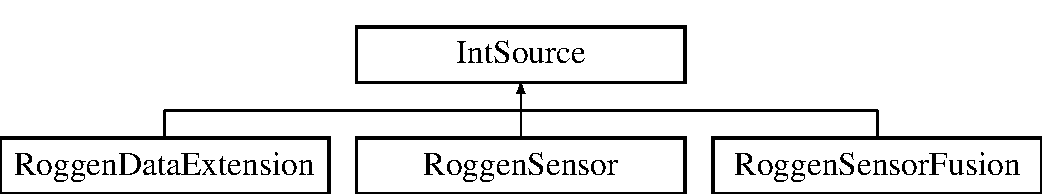
\includegraphics[height=2cm]{classIntSource}
\end{center}
\end{figure}
\subsection*{Public Member Functions}
\begin{DoxyCompactItemize}
\item 
\hypertarget{classIntSource_a0a3b7469b2d7d5165b55afc65511eecc}{
virtual std::vector$<$ std::vector$<$ int $>$ $>$ {\bfseries getData} ()=0}
\label{classIntSource_a0a3b7469b2d7d5165b55afc65511eecc}

\item 
virtual \hyperlink{classIntSource_a96642d807a1cb32cbb856cfe0f847542}{$\sim$IntSource} ()
\end{DoxyCompactItemize}


\subsection{Detailed Description}
Interface class: Every descendant has to offer a getData function. Example descendants are the sensor classes. Author: Lars Widmer, www.lawi.ch 

\subsection{Constructor \& Destructor Documentation}
\hypertarget{classIntSource_a96642d807a1cb32cbb856cfe0f847542}{
\index{IntSource@{IntSource}!$\sim$IntSource@{$\sim$IntSource}}
\index{$\sim$IntSource@{$\sim$IntSource}!IntSource@{IntSource}}
\subsubsection[{$\sim$IntSource}]{\setlength{\rightskip}{0pt plus 5cm}IntSource::$\sim$IntSource ()\hspace{0.3cm}{\ttfamily  \mbox{[}virtual\mbox{]}}}}
\label{classIntSource_a96642d807a1cb32cbb856cfe0f847542}
Empty destructor (virtual). Class is just an interface. 

The documentation for this class was generated from the following files:\begin{DoxyCompactItemize}
\item 
IntSource.h\item 
IntSource.cpp\end{DoxyCompactItemize}

\hypertarget{structIntStruct}{
\section{IntStruct Struct Reference}
\label{structIntStruct}\index{IntStruct@{IntStruct}}
}
\subsection*{Public Attributes}
\begin{DoxyCompactItemize}
\item 
\hypertarget{structIntStruct_ae60ea69678bdcb56beadb29b4ba869f0}{
IntVec {\bfseries vals}}
\label{structIntStruct_ae60ea69678bdcb56beadb29b4ba869f0}

\item 
\hypertarget{structIntStruct_a2a47e58e158f2763090285140893b1e9}{
StringVec {\bfseries defs}}
\label{structIntStruct_a2a47e58e158f2763090285140893b1e9}

\item 
\hypertarget{structIntStruct_ad71cb2d1f1990d8bf8a4bf7e8dd45f3c}{
std::string {\bfseries name}}
\label{structIntStruct_ad71cb2d1f1990d8bf8a4bf7e8dd45f3c}

\item 
\hypertarget{structIntStruct_a6a0c3098aa24ab4b59ed78e69422f371}{
int {\bfseries num}}
\label{structIntStruct_a6a0c3098aa24ab4b59ed78e69422f371}

\end{DoxyCompactItemize}


The documentation for this struct was generated from the following file:\begin{DoxyCompactItemize}
\item 
XmlFileHandling.h\end{DoxyCompactItemize}

\hypertarget{classLearningAlgorithm}{
\section{LearningAlgorithm Class Reference}
\label{classLearningAlgorithm}\index{LearningAlgorithm@{LearningAlgorithm}}
}
Inheritance diagram for LearningAlgorithm::\begin{figure}[H]
\begin{center}
\leavevmode
\includegraphics[height=2cm]{classLearningAlgorithm}
\end{center}
\end{figure}
\subsection*{Public Member Functions}
\begin{DoxyCompactItemize}
\item 
virtual \hyperlink{classLearningAlgorithm_a0ec630ac5340988eea92b8ede9a4422d}{$\sim$LearningAlgorithm} ()
\item 
\hypertarget{classLearningAlgorithm_a43578336f77312cfc2aac189034d9d78}{
virtual void {\bfseries reset} ()=0}
\label{classLearningAlgorithm_a43578336f77312cfc2aac189034d9d78}

\item 
\hypertarget{classLearningAlgorithm_a241f4be6894d83d6a61bfa0689fee874}{
virtual void {\bfseries train} (FeatureSet)=0}
\label{classLearningAlgorithm_a241f4be6894d83d6a61bfa0689fee874}

\item 
\hypertarget{classLearningAlgorithm_a5460eb0cc848daf0f84c5fc7093fe94b}{
virtual \hyperlink{structOutput}{Output} {\bfseries classify} (Features)=0}
\label{classLearningAlgorithm_a5460eb0cc848daf0f84c5fc7093fe94b}

\item 
\hypertarget{classLearningAlgorithm_a188698bec0d1d94f573521c9a0f1e831}{
virtual std::pair$<$ \hyperlink{structOutput}{Output}, FeatureType $>$ {\bfseries classification} (Features)=0}
\label{classLearningAlgorithm_a188698bec0d1d94f573521c9a0f1e831}

\item 
\hypertarget{classLearningAlgorithm_a77ba7b2046ba7015fca9f7f1262ca2f0}{
virtual void {\bfseries setUnknownThreshold} (float)=0}
\label{classLearningAlgorithm_a77ba7b2046ba7015fca9f7f1262ca2f0}

\item 
\hypertarget{classLearningAlgorithm_ab8294855692cdef11461c97942f6239f}{
virtual float {\bfseries getUnknownThreshold} ()=0}
\label{classLearningAlgorithm_ab8294855692cdef11461c97942f6239f}

\item 
\hypertarget{classLearningAlgorithm_aa2faa60adbe835f0748cb1b47f822379}{
virtual void {\bfseries print} ()=0}
\label{classLearningAlgorithm_aa2faa60adbe835f0748cb1b47f822379}

\end{DoxyCompactItemize}


\subsection{Constructor \& Destructor Documentation}
\hypertarget{classLearningAlgorithm_a0ec630ac5340988eea92b8ede9a4422d}{
\index{LearningAlgorithm@{LearningAlgorithm}!$\sim$LearningAlgorithm@{$\sim$LearningAlgorithm}}
\index{$\sim$LearningAlgorithm@{$\sim$LearningAlgorithm}!LearningAlgorithm@{LearningAlgorithm}}
\subsubsection[{$\sim$LearningAlgorithm}]{\setlength{\rightskip}{0pt plus 5cm}LearningAlgorithm::$\sim$LearningAlgorithm ()\hspace{0.3cm}{\ttfamily  \mbox{[}virtual\mbox{]}}}}
\label{classLearningAlgorithm_a0ec630ac5340988eea92b8ede9a4422d}
Pure interface class. Empty (virtual) destructor. 

The documentation for this class was generated from the following files:\begin{DoxyCompactItemize}
\item 
LearningAlgorithm.h\item 
LearningAlgorithm.cpp\end{DoxyCompactItemize}

\hypertarget{structLimbCoordinates}{
\section{LimbCoordinates Struct Reference}
\label{structLimbCoordinates}\index{LimbCoordinates@{LimbCoordinates}}
}
\subsection*{Public Attributes}
\begin{DoxyCompactItemize}
\item 
\hypertarget{structLimbCoordinates_ab2e4302ad3f0dca1b90c191372b369c9}{
float {\bfseries x}}
\label{structLimbCoordinates_ab2e4302ad3f0dca1b90c191372b369c9}

\item 
\hypertarget{structLimbCoordinates_ace36fd5842192df47b481d777cc1589e}{
float {\bfseries y}}
\label{structLimbCoordinates_ace36fd5842192df47b481d777cc1589e}

\item 
\hypertarget{structLimbCoordinates_ae367ee3e85baccb4be01c18a4c55510f}{
float {\bfseries z}}
\label{structLimbCoordinates_ae367ee3e85baccb4be01c18a4c55510f}

\end{DoxyCompactItemize}


The documentation for this struct was generated from the following file:\begin{DoxyCompactItemize}
\item 
Defines.h\end{DoxyCompactItemize}

\hypertarget{structLimbNameCoordinates}{
\section{LimbNameCoordinates Struct Reference}
\label{structLimbNameCoordinates}\index{LimbNameCoordinates@{LimbNameCoordinates}}
}
\subsection*{Public Attributes}
\begin{DoxyCompactItemize}
\item 
\hypertarget{structLimbNameCoordinates_a485a7e27de43cff1c12cf34e7f8e5033}{
std::string {\bfseries name}}
\label{structLimbNameCoordinates_a485a7e27de43cff1c12cf34e7f8e5033}

\item 
\hypertarget{structLimbNameCoordinates_acf052aeed78d87bea08b99e384bcf82f}{
float {\bfseries x}}
\label{structLimbNameCoordinates_acf052aeed78d87bea08b99e384bcf82f}

\item 
\hypertarget{structLimbNameCoordinates_ab652230e4417a0d18dfd98c9598310d7}{
float {\bfseries y}}
\label{structLimbNameCoordinates_ab652230e4417a0d18dfd98c9598310d7}

\item 
\hypertarget{structLimbNameCoordinates_a849a8dde9955fee392bf73aa6d874765}{
float {\bfseries z}}
\label{structLimbNameCoordinates_a849a8dde9955fee392bf73aa6d874765}

\end{DoxyCompactItemize}


The documentation for this struct was generated from the following file:\begin{DoxyCompactItemize}
\item 
Defines.h\end{DoxyCompactItemize}

\hypertarget{classMutex}{
\section{Mutex Class Reference}
\label{classMutex}\index{Mutex@{Mutex}}
}


{\ttfamily \#include $<$Mutex.h$>$}Inheritance diagram for Mutex::\begin{figure}[H]
\begin{center}
\leavevmode
\includegraphics[height=2cm]{classMutex}
\end{center}
\end{figure}
\subsection*{Public Member Functions}
\begin{DoxyCompactItemize}
\item 
\hyperlink{classMutex_a593423d868daf926c7b0d63a833ae29a}{Mutex} ()
\item 
virtual \hyperlink{classMutex_ac9e9182407f5f74892318607888e9be4}{$\sim$Mutex} ()
\item 
void \hyperlink{classMutex_a0f7dda8ab1e2ad808feacb3c9d7fc8ad}{acquireMutex} ()
\item 
void \hyperlink{classMutex_a2f4a3dd7d969f9d77e67ceea9cb6bc3a}{releaseMutex} ()
\end{DoxyCompactItemize}


\subsection{Detailed Description}
Simple class for inheritance or aggregation. It provides a single mutex (mutal exclusion). Using it as a super class is easier. Whereas aggregation has to be used in the case when more than one mutex is needed. Author: Lars Widmer, www.lawi.ch 

\subsection{Constructor \& Destructor Documentation}
\hypertarget{classMutex_a593423d868daf926c7b0d63a833ae29a}{
\index{Mutex@{Mutex}!Mutex@{Mutex}}
\index{Mutex@{Mutex}!Mutex@{Mutex}}
\subsubsection[{Mutex}]{\setlength{\rightskip}{0pt plus 5cm}Mutex::Mutex ()}}
\label{classMutex_a593423d868daf926c7b0d63a833ae29a}
Constructor: Initializes the mutual exclusion. \hypertarget{classMutex_ac9e9182407f5f74892318607888e9be4}{
\index{Mutex@{Mutex}!$\sim$Mutex@{$\sim$Mutex}}
\index{$\sim$Mutex@{$\sim$Mutex}!Mutex@{Mutex}}
\subsubsection[{$\sim$Mutex}]{\setlength{\rightskip}{0pt plus 5cm}Mutex::$\sim$Mutex ()\hspace{0.3cm}{\ttfamily  \mbox{[}virtual\mbox{]}}}}
\label{classMutex_ac9e9182407f5f74892318607888e9be4}
Destructor: Destroys the mutual exclusion. 

\subsection{Member Function Documentation}
\hypertarget{classMutex_a0f7dda8ab1e2ad808feacb3c9d7fc8ad}{
\index{Mutex@{Mutex}!acquireMutex@{acquireMutex}}
\index{acquireMutex@{acquireMutex}!Mutex@{Mutex}}
\subsubsection[{acquireMutex}]{\setlength{\rightskip}{0pt plus 5cm}void Mutex::acquireMutex ()}}
\label{classMutex_a0f7dda8ab1e2ad808feacb3c9d7fc8ad}
Acquire the mutual exclusion. \hypertarget{classMutex_a2f4a3dd7d969f9d77e67ceea9cb6bc3a}{
\index{Mutex@{Mutex}!releaseMutex@{releaseMutex}}
\index{releaseMutex@{releaseMutex}!Mutex@{Mutex}}
\subsubsection[{releaseMutex}]{\setlength{\rightskip}{0pt plus 5cm}void Mutex::releaseMutex ()}}
\label{classMutex_a2f4a3dd7d969f9d77e67ceea9cb6bc3a}
Release the mutual exclusion. 

The documentation for this class was generated from the following files:\begin{DoxyCompactItemize}
\item 
Mutex.h\item 
Mutex.cpp\end{DoxyCompactItemize}

\hypertarget{classNearestClusterCenter}{
\section{NearestClusterCenter Class Reference}
\label{classNearestClusterCenter}\index{NearestClusterCenter@{NearestClusterCenter}}
}
Inheritance diagram for NearestClusterCenter::\begin{figure}[H]
\begin{center}
\leavevmode
\includegraphics[height=2cm]{classNearestClusterCenter}
\end{center}
\end{figure}
\subsection*{Public Member Functions}
\begin{DoxyCompactItemize}
\item 
\hyperlink{classNearestClusterCenter_a91e3450a7df8ef80a80ea9803671bb1e}{NearestClusterCenter} ()
\item 
\hyperlink{classNearestClusterCenter_ae3f8e71ca34ae2e0187395c38045f041}{NearestClusterCenter} (FeatureSet)
\item 
virtual \hyperlink{classNearestClusterCenter_a8b6f7f60937d0e860b117d774d645928}{$\sim$NearestClusterCenter} ()
\item 
virtual void \hyperlink{classNearestClusterCenter_ab5f85125ff65850ca4673fa0e85a0af5}{reset} ()
\item 
virtual void \hyperlink{classNearestClusterCenter_af3a9ba6b9ef3fb453ff10e76fe34e9d4}{train} (FeatureSet)
\item 
virtual \hyperlink{structOutput}{Output} \hyperlink{classNearestClusterCenter_ad2df5aaa3dabc0ef398a24872937b878}{classify} (Features)
\item 
virtual std::pair$<$ \hyperlink{structOutput}{Output}, FeatureType $>$ \hyperlink{classNearestClusterCenter_a49853a2af22ba1688ac438a376d53c42}{classification} (Features)
\item 
virtual void \hyperlink{classNearestClusterCenter_ab902e7abfb704d132d8548672253bb0a}{setUnknownThreshold} (float)
\item 
virtual float \hyperlink{classNearestClusterCenter_aad9b89686794d4b974b38e3aac7bb51e}{getUnknownThreshold} ()
\item 
virtual void \hyperlink{classNearestClusterCenter_a9ae11b14356f29dcf5fa2666dac6faed}{print} ()
\end{DoxyCompactItemize}


\subsection{Constructor \& Destructor Documentation}
\hypertarget{classNearestClusterCenter_a91e3450a7df8ef80a80ea9803671bb1e}{
\index{NearestClusterCenter@{NearestClusterCenter}!NearestClusterCenter@{NearestClusterCenter}}
\index{NearestClusterCenter@{NearestClusterCenter}!NearestClusterCenter@{NearestClusterCenter}}
\subsubsection[{NearestClusterCenter}]{\setlength{\rightskip}{0pt plus 5cm}NearestClusterCenter::NearestClusterCenter ()}}
\label{classNearestClusterCenter_a91e3450a7df8ef80a80ea9803671bb1e}
Constructor: Clears all the internal fields and leaves the algorithm untrained. \hypertarget{classNearestClusterCenter_ae3f8e71ca34ae2e0187395c38045f041}{
\index{NearestClusterCenter@{NearestClusterCenter}!NearestClusterCenter@{NearestClusterCenter}}
\index{NearestClusterCenter@{NearestClusterCenter}!NearestClusterCenter@{NearestClusterCenter}}
\subsubsection[{NearestClusterCenter}]{\setlength{\rightskip}{0pt plus 5cm}NearestClusterCenter::NearestClusterCenter (FeatureSet {\em s})}}
\label{classNearestClusterCenter_ae3f8e71ca34ae2e0187395c38045f041}
Constructor: Clears all the internal fields and trains the algorithm with the given set of features. \hypertarget{classNearestClusterCenter_a8b6f7f60937d0e860b117d774d645928}{
\index{NearestClusterCenter@{NearestClusterCenter}!$\sim$NearestClusterCenter@{$\sim$NearestClusterCenter}}
\index{$\sim$NearestClusterCenter@{$\sim$NearestClusterCenter}!NearestClusterCenter@{NearestClusterCenter}}
\subsubsection[{$\sim$NearestClusterCenter}]{\setlength{\rightskip}{0pt plus 5cm}NearestClusterCenter::$\sim$NearestClusterCenter ()\hspace{0.3cm}{\ttfamily  \mbox{[}virtual\mbox{]}}}}
\label{classNearestClusterCenter_a8b6f7f60937d0e860b117d774d645928}
Empty Destructor 

\subsection{Member Function Documentation}
\hypertarget{classNearestClusterCenter_a49853a2af22ba1688ac438a376d53c42}{
\index{NearestClusterCenter@{NearestClusterCenter}!classification@{classification}}
\index{classification@{classification}!NearestClusterCenter@{NearestClusterCenter}}
\subsubsection[{classification}]{\setlength{\rightskip}{0pt plus 5cm}pair$<$ {\bf Output}, FeatureType $>$ NearestClusterCenter::classification (Features {\em in})\hspace{0.3cm}{\ttfamily  \mbox{[}virtual\mbox{]}}}}
\label{classNearestClusterCenter_a49853a2af22ba1688ac438a376d53c42}
Classification function. Matches the given point in feature space to the nearest cluster center. The classification is marked valid depending if the distance between the point and the center is less then the defined threshold. The first value of the output pair is the found classification in an \hyperlink{structOutput}{Output} struct. The \hyperlink{structOutput}{Output} struct contains a flag if the classification is valid and the value of the classification. The second value of the output pair tells the distance between the given point and the matched cluster center. 

Implements \hyperlink{classLearningAlgorithm}{LearningAlgorithm}.\hypertarget{classNearestClusterCenter_ad2df5aaa3dabc0ef398a24872937b878}{
\index{NearestClusterCenter@{NearestClusterCenter}!classify@{classify}}
\index{classify@{classify}!NearestClusterCenter@{NearestClusterCenter}}
\subsubsection[{classify}]{\setlength{\rightskip}{0pt plus 5cm}{\bf Output} NearestClusterCenter::classify (Features {\em in})\hspace{0.3cm}{\ttfamily  \mbox{[}virtual\mbox{]}}}}
\label{classNearestClusterCenter_ad2df5aaa3dabc0ef398a24872937b878}
Classification function. Matches the given point in feature space to the nearest cluster center. The classification is marked valid depending if the distance between the point and the center is less then the defined threshold. The return value is the found classification as an \hyperlink{structOutput}{Output} struct. The \hyperlink{structOutput}{Output} struct contains a flag if the classification is valid and the value of the classification. 

Implements \hyperlink{classLearningAlgorithm}{LearningAlgorithm}.\hypertarget{classNearestClusterCenter_aad9b89686794d4b974b38e3aac7bb51e}{
\index{NearestClusterCenter@{NearestClusterCenter}!getUnknownThreshold@{getUnknownThreshold}}
\index{getUnknownThreshold@{getUnknownThreshold}!NearestClusterCenter@{NearestClusterCenter}}
\subsubsection[{getUnknownThreshold}]{\setlength{\rightskip}{0pt plus 5cm}float NearestClusterCenter::getUnknownThreshold ()\hspace{0.3cm}{\ttfamily  \mbox{[}virtual\mbox{]}}}}
\label{classNearestClusterCenter_aad9b89686794d4b974b38e3aac7bb51e}
Getter function for the classification threshold. If a point in feature space is classified with a distance from the nearest cluster bigger then the threshold it's marked as invalid. 

Implements \hyperlink{classLearningAlgorithm}{LearningAlgorithm}.\hypertarget{classNearestClusterCenter_a9ae11b14356f29dcf5fa2666dac6faed}{
\index{NearestClusterCenter@{NearestClusterCenter}!print@{print}}
\index{print@{print}!NearestClusterCenter@{NearestClusterCenter}}
\subsubsection[{print}]{\setlength{\rightskip}{0pt plus 5cm}void NearestClusterCenter::print ()\hspace{0.3cm}{\ttfamily  \mbox{[}virtual\mbox{]}}}}
\label{classNearestClusterCenter_a9ae11b14356f29dcf5fa2666dac6faed}
Print function for the set of cluster centers. 

Implements \hyperlink{classLearningAlgorithm}{LearningAlgorithm}.\hypertarget{classNearestClusterCenter_ab5f85125ff65850ca4673fa0e85a0af5}{
\index{NearestClusterCenter@{NearestClusterCenter}!reset@{reset}}
\index{reset@{reset}!NearestClusterCenter@{NearestClusterCenter}}
\subsubsection[{reset}]{\setlength{\rightskip}{0pt plus 5cm}void NearestClusterCenter::reset ()\hspace{0.3cm}{\ttfamily  \mbox{[}virtual\mbox{]}}}}
\label{classNearestClusterCenter_ab5f85125ff65850ca4673fa0e85a0af5}
Clears the internal fields e.g. resets the training state to untrained. 

Implements \hyperlink{classLearningAlgorithm}{LearningAlgorithm}.\hypertarget{classNearestClusterCenter_ab902e7abfb704d132d8548672253bb0a}{
\index{NearestClusterCenter@{NearestClusterCenter}!setUnknownThreshold@{setUnknownThreshold}}
\index{setUnknownThreshold@{setUnknownThreshold}!NearestClusterCenter@{NearestClusterCenter}}
\subsubsection[{setUnknownThreshold}]{\setlength{\rightskip}{0pt plus 5cm}void NearestClusterCenter::setUnknownThreshold (float {\em newUT})\hspace{0.3cm}{\ttfamily  \mbox{[}virtual\mbox{]}}}}
\label{classNearestClusterCenter_ab902e7abfb704d132d8548672253bb0a}
Setter function for the classification threshold. If a point in feature space is classified with a distance from the nearest cluster bigger then the threshold it's marked as invalid. 

Implements \hyperlink{classLearningAlgorithm}{LearningAlgorithm}.\hypertarget{classNearestClusterCenter_af3a9ba6b9ef3fb453ff10e76fe34e9d4}{
\index{NearestClusterCenter@{NearestClusterCenter}!train@{train}}
\index{train@{train}!NearestClusterCenter@{NearestClusterCenter}}
\subsubsection[{train}]{\setlength{\rightskip}{0pt plus 5cm}void NearestClusterCenter::train (FeatureSet {\em set})\hspace{0.3cm}{\ttfamily  \mbox{[}virtual\mbox{]}}}}
\label{classNearestClusterCenter_af3a9ba6b9ef3fb453ff10e76fe34e9d4}
Trains the algorithm with the given training set. 

Implements \hyperlink{classLearningAlgorithm}{LearningAlgorithm}.

The documentation for this class was generated from the following files:\begin{DoxyCompactItemize}
\item 
NearestClusterCenter.h\item 
NearestClusterCenter.cpp\end{DoxyCompactItemize}

\hypertarget{structNeighbour}{
\section{Neighbour Struct Reference}
\label{structNeighbour}\index{Neighbour@{Neighbour}}
}
\subsection*{Public Attributes}
\begin{DoxyCompactItemize}
\item 
\hypertarget{structNeighbour_a136bbd389de0f83ee837f790128c976c}{
CoordSet {\bfseries positions}}
\label{structNeighbour_a136bbd389de0f83ee837f790128c976c}

\item 
\hypertarget{structNeighbour_ac53c620b5efef290cf8bdc2474353243}{
std::string {\bfseries name}}
\label{structNeighbour_ac53c620b5efef290cf8bdc2474353243}

\end{DoxyCompactItemize}


The documentation for this struct was generated from the following file:\begin{DoxyCompactItemize}
\item 
XmlFileHandling.h\end{DoxyCompactItemize}

\hypertarget{structNodeAndData}{
\section{NodeAndData Struct Reference}
\label{structNodeAndData}\index{NodeAndData@{NodeAndData}}
}
\subsection*{Public Attributes}
\begin{DoxyCompactItemize}
\item 
\hypertarget{structNodeAndData_aac0364aa0f250fc253a70713849c2085}{
\hyperlink{structNodeData}{NodeData} {\bfseries data}}
\label{structNodeAndData_aac0364aa0f250fc253a70713849c2085}

\item 
\hypertarget{structNodeAndData_acad67c8ca3ed7bf54964702746341797}{
int {\bfseries node}}
\label{structNodeAndData_acad67c8ca3ed7bf54964702746341797}

\end{DoxyCompactItemize}


The documentation for this struct was generated from the following file:\begin{DoxyCompactItemize}
\item 
Defines.h\end{DoxyCompactItemize}

\hypertarget{structNodeData}{
\section{NodeData Struct Reference}
\label{structNodeData}\index{NodeData@{NodeData}}
}
\subsection*{Public Attributes}
\begin{DoxyCompactItemize}
\item 
\hypertarget{structNodeData_ac223d38b9dba2817057adc7c3a41bce9}{
float {\bfseries accX}}
\label{structNodeData_ac223d38b9dba2817057adc7c3a41bce9}

\item 
\hypertarget{structNodeData_ae448efdff89ae766a3e18a9df6ad23f5}{
float {\bfseries accY}}
\label{structNodeData_ae448efdff89ae766a3e18a9df6ad23f5}

\item 
\hypertarget{structNodeData_aa200421c0824b0120a35394143bac5ce}{
float {\bfseries accZ}}
\label{structNodeData_aa200421c0824b0120a35394143bac5ce}

\item 
\hypertarget{structNodeData_aec218c69255eb692ff41049c507cf08d}{
float {\bfseries magX}}
\label{structNodeData_aec218c69255eb692ff41049c507cf08d}

\item 
\hypertarget{structNodeData_a2028552722bfa03682999db9c79b199e}{
float {\bfseries magY}}
\label{structNodeData_a2028552722bfa03682999db9c79b199e}

\item 
\hypertarget{structNodeData_ab134ba2060337c908d2bd6fdb7c132ff}{
float {\bfseries magZ}}
\label{structNodeData_ab134ba2060337c908d2bd6fdb7c132ff}

\item 
\hypertarget{structNodeData_a87552f3659f4d64e1ddb07bc03b7a36f}{
float {\bfseries volts}}
\label{structNodeData_a87552f3659f4d64e1ddb07bc03b7a36f}

\item 
\hypertarget{structNodeData_aa90953affd189f1c02295c12cec5f3ba}{
bool {\bfseries valid}}
\label{structNodeData_aa90953affd189f1c02295c12cec5f3ba}

\end{DoxyCompactItemize}


The documentation for this struct was generated from the following file:\begin{DoxyCompactItemize}
\item 
Defines.h\end{DoxyCompactItemize}

\hypertarget{structOutput}{
\section{Output Struct Reference}
\label{structOutput}\index{Output@{Output}}
}
\subsection*{Public Attributes}
\begin{DoxyCompactItemize}
\item 
\hypertarget{structOutput_acbf2c8185d69204b63721d29b3cfda2b}{
OutputType {\bfseries value}}
\label{structOutput_acbf2c8185d69204b63721d29b3cfda2b}

\item 
\hypertarget{structOutput_a10571ec61994587513a0fbd40d94bc30}{
bool {\bfseries valid}}
\label{structOutput_a10571ec61994587513a0fbd40d94bc30}

\end{DoxyCompactItemize}


The documentation for this struct was generated from the following file:\begin{DoxyCompactItemize}
\item 
LearningAlgorithm.h\end{DoxyCompactItemize}

\hypertarget{classRepercussion}{
\section{Repercussion Class Reference}
\label{classRepercussion}\index{Repercussion@{Repercussion}}
}


{\ttfamily \#include $<$Repercussion.h$>$}Inheritance diagram for Repercussion::\begin{figure}[H]
\begin{center}
\leavevmode
\includegraphics[height=2cm]{classRepercussion}
\end{center}
\end{figure}
\subsection*{Public Member Functions}
\begin{DoxyCompactItemize}
\item 
\hyperlink{classRepercussion_aa00feedc0ca2b0b3f75e799cd4dc4dac}{Repercussion} ()
\item 
\hyperlink{classRepercussion_a5a89f900156f4074a3d569fe48b11f1d}{Repercussion} (int)
\item 
virtual \hyperlink{classRepercussion_ad32730687e044c8d774dfb995af2f5a8}{$\sim$Repercussion} ()
\item 
void \hyperlink{classRepercussion_a903a946946c3393ea3a063d594e0fb91}{threadMethod} ()
\item 
void \hyperlink{classRepercussion_a27ded768fd7b386d8530dae787c46911}{set} (int, int=1)
\item 
int \hyperlink{classRepercussion_a1841959db6918b0bacdd436ef56b8313}{get} (int)
\item 
void \hyperlink{classRepercussion_ad119f81fef26097425bed1cad45dcaa9}{resetAll} ()
\item 
void \hyperlink{classRepercussion_a5677645d06730a42d44b2b69e6e1cac2}{reset} (int)
\item 
void \hyperlink{classRepercussion_aaa27e3c9251d0dda1c24ac77421bdaab}{inc} (int, int=1)
\item 
void \hyperlink{classRepercussion_ac86fbba0711b097da755b6a7280eef63}{dec} (int, int=1)
\item 
void \hyperlink{classRepercussion_afece2a141e05cceea3dff10b7d67c63e}{incAll} (int=1)
\item 
void \hyperlink{classRepercussion_ad825c06913e11c2617f38ee4421f237a}{setAll} (int=1)
\item 
void \hyperlink{classRepercussion_a87bb91156e63992084f6011b32acab8c}{decAll} (int=1)
\item 
std::vector$<$ int $>$ \hyperlink{classRepercussion_af2d97e8c5795fb6df793e0f17dd4831d}{getAll} ()
\item 
bool \hyperlink{classRepercussion_a95fc77c0adf534f0ce92a48a23bdaece}{isZero} (int)
\item 
void \hyperlink{classRepercussion_a19b9c3950397311c5f275fce451df5f6}{activate} ()
\item 
void \hyperlink{classRepercussion_a0d1bcb6ab372efecb912006e038f2bd5}{deactivate} ()
\item 
void \hyperlink{classRepercussion_a046c98f4950c6f484cb5d07c5f295e23}{setDelay} (int)
\item 
void \hyperlink{classRepercussion_a66219691fbf748e8751cf1c447347683}{setDecrement} (int)
\item 
void \hyperlink{classRepercussion_a8f4c193ca2406c92ebff923218c2e328}{setMaximum} (int)
\end{DoxyCompactItemize}


\subsection{Detailed Description}
Class for managing values which decrease against time. It can be used to make single events lasting over a defined amount of time. Author: Lars Widmer, www.lawi.ch 

\subsection{Constructor \& Destructor Documentation}
\hypertarget{classRepercussion_aa00feedc0ca2b0b3f75e799cd4dc4dac}{
\index{Repercussion@{Repercussion}!Repercussion@{Repercussion}}
\index{Repercussion@{Repercussion}!Repercussion@{Repercussion}}
\subsubsection[{Repercussion}]{\setlength{\rightskip}{0pt plus 5cm}Repercussion::Repercussion ()}}
\label{classRepercussion_aa00feedc0ca2b0b3f75e799cd4dc4dac}
Constructor creates and initializes an empty instance. \hypertarget{classRepercussion_a5a89f900156f4074a3d569fe48b11f1d}{
\index{Repercussion@{Repercussion}!Repercussion@{Repercussion}}
\index{Repercussion@{Repercussion}!Repercussion@{Repercussion}}
\subsubsection[{Repercussion}]{\setlength{\rightskip}{0pt plus 5cm}Repercussion::Repercussion (int {\em number})}}
\label{classRepercussion_a5a89f900156f4074a3d569fe48b11f1d}
Constructor creates and initializes an instance for the use with the given number of values. \hypertarget{classRepercussion_ad32730687e044c8d774dfb995af2f5a8}{
\index{Repercussion@{Repercussion}!$\sim$Repercussion@{$\sim$Repercussion}}
\index{$\sim$Repercussion@{$\sim$Repercussion}!Repercussion@{Repercussion}}
\subsubsection[{$\sim$Repercussion}]{\setlength{\rightskip}{0pt plus 5cm}Repercussion::$\sim$Repercussion ()\hspace{0.3cm}{\ttfamily  \mbox{[}virtual\mbox{]}}}}
\label{classRepercussion_ad32730687e044c8d774dfb995af2f5a8}
Destructor: Stops the internal thread. 

\subsection{Member Function Documentation}
\hypertarget{classRepercussion_a19b9c3950397311c5f275fce451df5f6}{
\index{Repercussion@{Repercussion}!activate@{activate}}
\index{activate@{activate}!Repercussion@{Repercussion}}
\subsubsection[{activate}]{\setlength{\rightskip}{0pt plus 5cm}void Repercussion::activate ()}}
\label{classRepercussion_a19b9c3950397311c5f275fce451df5f6}
Activates the repercussion instance. Initially the instance of this class is inactive. It doesn't start decrementing before it's activated. First define all the settings and then activate. \hypertarget{classRepercussion_a0d1bcb6ab372efecb912006e038f2bd5}{
\index{Repercussion@{Repercussion}!deactivate@{deactivate}}
\index{deactivate@{deactivate}!Repercussion@{Repercussion}}
\subsubsection[{deactivate}]{\setlength{\rightskip}{0pt plus 5cm}void Repercussion::deactivate ()}}
\label{classRepercussion_a0d1bcb6ab372efecb912006e038f2bd5}
Deactivates the repercussion instance. It doesn't decrement while inactive. \hypertarget{classRepercussion_ac86fbba0711b097da755b6a7280eef63}{
\index{Repercussion@{Repercussion}!dec@{dec}}
\index{dec@{dec}!Repercussion@{Repercussion}}
\subsubsection[{dec}]{\setlength{\rightskip}{0pt plus 5cm}void Repercussion::dec (int {\em val}, \/  int {\em amount} = {\ttfamily 1})}}
\label{classRepercussion_ac86fbba0711b097da755b6a7280eef63}
Subtract the amount given in the second parameter from the value with the index given in the first parameter. With this method the values can't get negative. \hypertarget{classRepercussion_a87bb91156e63992084f6011b32acab8c}{
\index{Repercussion@{Repercussion}!decAll@{decAll}}
\index{decAll@{decAll}!Repercussion@{Repercussion}}
\subsubsection[{decAll}]{\setlength{\rightskip}{0pt plus 5cm}void Repercussion::decAll (int {\em amount} = {\ttfamily 1})}}
\label{classRepercussion_a87bb91156e63992084f6011b32acab8c}
Subtract the given amount from all values. With this method the values can't get negative. \hypertarget{classRepercussion_a1841959db6918b0bacdd436ef56b8313}{
\index{Repercussion@{Repercussion}!get@{get}}
\index{get@{get}!Repercussion@{Repercussion}}
\subsubsection[{get}]{\setlength{\rightskip}{0pt plus 5cm}int Repercussion::get (int {\em val})}}
\label{classRepercussion_a1841959db6918b0bacdd436ef56b8313}
Return the value with the given index. \hypertarget{classRepercussion_af2d97e8c5795fb6df793e0f17dd4831d}{
\index{Repercussion@{Repercussion}!getAll@{getAll}}
\index{getAll@{getAll}!Repercussion@{Repercussion}}
\subsubsection[{getAll}]{\setlength{\rightskip}{0pt plus 5cm}std::vector$<$ int $>$ Repercussion::getAll ()}}
\label{classRepercussion_af2d97e8c5795fb6df793e0f17dd4831d}
Returns all the values as a vector. \hypertarget{classRepercussion_aaa27e3c9251d0dda1c24ac77421bdaab}{
\index{Repercussion@{Repercussion}!inc@{inc}}
\index{inc@{inc}!Repercussion@{Repercussion}}
\subsubsection[{inc}]{\setlength{\rightskip}{0pt plus 5cm}void Repercussion::inc (int {\em val}, \/  int {\em amount} = {\ttfamily 1})}}
\label{classRepercussion_aaa27e3c9251d0dda1c24ac77421bdaab}
Add the amount given in the second parameter to the value with the index given in the first parameter. With this method the values can't go over the defined maximum. \hypertarget{classRepercussion_afece2a141e05cceea3dff10b7d67c63e}{
\index{Repercussion@{Repercussion}!incAll@{incAll}}
\index{incAll@{incAll}!Repercussion@{Repercussion}}
\subsubsection[{incAll}]{\setlength{\rightskip}{0pt plus 5cm}void Repercussion::incAll (int {\em amount} = {\ttfamily 1})}}
\label{classRepercussion_afece2a141e05cceea3dff10b7d67c63e}
Add the given amount to all values. With this method the values can't go over the defined maximum. \hypertarget{classRepercussion_a95fc77c0adf534f0ce92a48a23bdaece}{
\index{Repercussion@{Repercussion}!isZero@{isZero}}
\index{isZero@{isZero}!Repercussion@{Repercussion}}
\subsubsection[{isZero}]{\setlength{\rightskip}{0pt plus 5cm}bool Repercussion::isZero (int {\em val})}}
\label{classRepercussion_a95fc77c0adf534f0ce92a48a23bdaece}
Returns true if the value with the given index is zero (or below). \hypertarget{classRepercussion_a5677645d06730a42d44b2b69e6e1cac2}{
\index{Repercussion@{Repercussion}!reset@{reset}}
\index{reset@{reset}!Repercussion@{Repercussion}}
\subsubsection[{reset}]{\setlength{\rightskip}{0pt plus 5cm}void Repercussion::reset (int {\em val})}}
\label{classRepercussion_a5677645d06730a42d44b2b69e6e1cac2}
Reset the value with the given index number to zero. \hypertarget{classRepercussion_ad119f81fef26097425bed1cad45dcaa9}{
\index{Repercussion@{Repercussion}!resetAll@{resetAll}}
\index{resetAll@{resetAll}!Repercussion@{Repercussion}}
\subsubsection[{resetAll}]{\setlength{\rightskip}{0pt plus 5cm}void Repercussion::resetAll ()}}
\label{classRepercussion_ad119f81fef26097425bed1cad45dcaa9}
Reset all values to zero. \hypertarget{classRepercussion_a27ded768fd7b386d8530dae787c46911}{
\index{Repercussion@{Repercussion}!set@{set}}
\index{set@{set}!Repercussion@{Repercussion}}
\subsubsection[{set}]{\setlength{\rightskip}{0pt plus 5cm}void Repercussion::set (int {\em val}, \/  int {\em level} = {\ttfamily 1})}}
\label{classRepercussion_a27ded768fd7b386d8530dae787c46911}
Set the value with the given index to the given level. \hypertarget{classRepercussion_ad825c06913e11c2617f38ee4421f237a}{
\index{Repercussion@{Repercussion}!setAll@{setAll}}
\index{setAll@{setAll}!Repercussion@{Repercussion}}
\subsubsection[{setAll}]{\setlength{\rightskip}{0pt plus 5cm}void Repercussion::setAll (int {\em level} = {\ttfamily 1})}}
\label{classRepercussion_ad825c06913e11c2617f38ee4421f237a}
Set all values to the given level. \hypertarget{classRepercussion_a66219691fbf748e8751cf1c447347683}{
\index{Repercussion@{Repercussion}!setDecrement@{setDecrement}}
\index{setDecrement@{setDecrement}!Repercussion@{Repercussion}}
\subsubsection[{setDecrement}]{\setlength{\rightskip}{0pt plus 5cm}void Repercussion::setDecrement (int {\em subtr})}}
\label{classRepercussion_a66219691fbf748e8751cf1c447347683}
Setter function for the amount to subtract from the values in each step. Default is 1. \hypertarget{classRepercussion_a046c98f4950c6f484cb5d07c5f295e23}{
\index{Repercussion@{Repercussion}!setDelay@{setDelay}}
\index{setDelay@{setDelay}!Repercussion@{Repercussion}}
\subsubsection[{setDelay}]{\setlength{\rightskip}{0pt plus 5cm}void Repercussion::setDelay (int {\em uSec})}}
\label{classRepercussion_a046c98f4950c6f484cb5d07c5f295e23}
Setter function for the delay in microseconds between the decrementation steps. Use values above 1000. Default is 1000. \hypertarget{classRepercussion_a8f4c193ca2406c92ebff923218c2e328}{
\index{Repercussion@{Repercussion}!setMaximum@{setMaximum}}
\index{setMaximum@{setMaximum}!Repercussion@{Repercussion}}
\subsubsection[{setMaximum}]{\setlength{\rightskip}{0pt plus 5cm}void Repercussion::setMaximum (int {\em max})}}
\label{classRepercussion_a8f4c193ca2406c92ebff923218c2e328}
Setter function for the maximum value. Default is 500. \hypertarget{classRepercussion_a903a946946c3393ea3a063d594e0fb91}{
\index{Repercussion@{Repercussion}!threadMethod@{threadMethod}}
\index{threadMethod@{threadMethod}!Repercussion@{Repercussion}}
\subsubsection[{threadMethod}]{\setlength{\rightskip}{0pt plus 5cm}void Repercussion::threadMethod ()\hspace{0.3cm}{\ttfamily  \mbox{[}virtual\mbox{]}}}}
\label{classRepercussion_a903a946946c3393ea3a063d594e0fb91}
\hyperlink{classThread}{Thread} method aging the stored values according to the defined settings. 

Reimplemented from \hyperlink{classThread_adc91220b96d25109b5f3ea73f8a75947}{Thread}.

The documentation for this class was generated from the following files:\begin{DoxyCompactItemize}
\item 
Repercussion.h\item 
Repercussion.cpp\end{DoxyCompactItemize}

\hypertarget{classRoggenBuffer}{
\section{RoggenBuffer Class Reference}
\label{classRoggenBuffer}\index{RoggenBuffer@{RoggenBuffer}}
}
\subsection*{Public Member Functions}
\begin{DoxyCompactItemize}
\item 
\hyperlink{classRoggenBuffer_a64573713834ff7772db6e180d9b34be6}{RoggenBuffer} ()
\item 
\hyperlink{classRoggenBuffer_a54b6110634f1f2d1a38552d58b841bf8}{RoggenBuffer} (std::vector$<$ std::vector$<$ int $>$ $>$)
\item 
\hyperlink{classRoggenBuffer_aaff7360a2f18576aeb9a5164a6cf6eec}{RoggenBuffer} (int)
\item 
virtual \hyperlink{classRoggenBuffer_a575b9194c53270add2d11e119d070293}{$\sim$RoggenBuffer} ()
\item 
std::vector$<$ std::vector$<$ int $>$ $>$ $\ast$ \hyperlink{classRoggenBuffer_a5fab9575ec2f4038c394009f689bffb7}{getPointer} ()
\item 
std::vector$<$ std::vector$<$ int $>$ $>$ \hyperlink{classRoggenBuffer_ad952a6eec2e3aea2a071f191c0decd36}{getRange} (int, int)
\item 
std::vector$<$ std::vector$<$ int $>$ $>$ \hyperlink{classRoggenBuffer_a7e4c7aa19aa7c900e2bbf00d23c698a1}{get} ()
\item 
std::vector$<$ std::vector$<$ int $>$ $>$ \hyperlink{classRoggenBuffer_a1c1ee753d0654159c62a0ee4ae95d9a0}{getLast} ()
\item 
bool \hyperlink{classRoggenBuffer_a1e2fe9957cfdf7db79678d929809efb0}{isFresh} ()
\item 
void \hyperlink{classRoggenBuffer_a199b6d0b632b4d9447a2ad85514d0872}{clear} ()
\item 
void \hyperlink{classRoggenBuffer_ad37f32dca74267b357a68c781920b08b}{setLength} (int)
\item 
int \hyperlink{classRoggenBuffer_aa74b37a710412767fa3bfcbf7f7c1958}{size} ()
\item 
int \hyperlink{classRoggenBuffer_ad64ee4593f5d4c488f3f18a9c0c558ab}{maxSize} ()
\item 
bool \hyperlink{classRoggenBuffer_a7eefcb649046e2e5929b76c890b07269}{isFull} ()
\item 
std::vector$<$ int $>$ \hyperlink{classRoggenBuffer_a81e4f32e486a0ae052bbe25088ccaffc}{at} (int)
\item 
\hypertarget{classRoggenBuffer_adcbbd2883819c7af9cf20ed95bbeb563}{
void {\bfseries put} (std::vector$<$ int $>$)}
\label{classRoggenBuffer_adcbbd2883819c7af9cf20ed95bbeb563}

\item 
\hypertarget{classRoggenBuffer_a0c49c7ea05d56f174e255dfee8664548}{
void {\bfseries put} (std::vector$<$ std::vector$<$ int $>$ $>$)}
\label{classRoggenBuffer_a0c49c7ea05d56f174e255dfee8664548}

\item 
std::vector$<$ int $>$ \hyperlink{classRoggenBuffer_a08b39243af623747c975c4d92d9a62cd}{getSingleMeasurement} (int)
\item 
std::vector$<$ std::vector$<$ int $>$ $>$ \hyperlink{classRoggenBuffer_a466876e9c5f87bf762467c97ae907048}{getFrames} (int, int)
\item 
void \hyperlink{classRoggenBuffer_a52b15812bb64d1821cbdce1646eab154}{checkSize} (int)
\item 
void \hyperlink{classRoggenBuffer_ad261de53f0e675cc0ed6a704991749c8}{check} (int, int)
\item 
std::vector$<$ std::vector$<$ int $>$ $>$ \hyperlink{classRoggenBuffer_ad1380e701fa8f05486c2f487e6740667}{filter} (int, int)
\item 
void \hyperlink{classRoggenBuffer_a42941bfb6c6319a1317f5da3c670facf}{filterPut} (int, int, std::vector$<$ int $>$)
\item 
void \hyperlink{classRoggenBuffer_a22ac37e59b6943d9f1996a43e58af190}{filterPut} (int, int, std::vector$<$ std::vector$<$ int $>$ $>$)
\item 
void \hyperlink{classRoggenBuffer_a86fe403735010ca3d62dbde7de22c0f3}{setUnlimited} ()
\item 
void \hyperlink{classRoggenBuffer_a252d46936fdf42d67af3f0e28a9c43c2}{resetUnlimited} ()
\item 
void \hyperlink{classRoggenBuffer_a3c0a581a4b554b63ad6ed8a1ee8c4d19}{setUnlimited} (bool flag)
\end{DoxyCompactItemize}
\subsection*{Static Public Member Functions}
\begin{DoxyCompactItemize}
\item 
\hypertarget{classRoggenBuffer_a6d6d0d7e81c2bc086278bbf88a4a41a0}{
static std::vector$<$ int $>$ {\bfseries getSingleMeasurement} (int, std::vector$<$ std::vector$<$ int $>$ $>$)}
\label{classRoggenBuffer_a6d6d0d7e81c2bc086278bbf88a4a41a0}

\item 
\hypertarget{classRoggenBuffer_a4d137aded6fd7477c6884440aeb0ceb1}{
static std::vector$<$ std::vector$<$ int $>$ $>$ {\bfseries getFrames} (int, int, std::vector$<$ std::vector$<$ int $>$ $>$)}
\label{classRoggenBuffer_a4d137aded6fd7477c6884440aeb0ceb1}

\item 
\hypertarget{classRoggenBuffer_a2dbeae26b5d0b862a3678c72aabf1e7d}{
static std::vector$<$ int $>$ {\bfseries getSum} (std::vector$<$ int $>$, std::vector$<$ int $>$)}
\label{classRoggenBuffer_a2dbeae26b5d0b862a3678c72aabf1e7d}

\item 
\hypertarget{classRoggenBuffer_ab04af345c5d1610685f47403ccf6485e}{
static std::vector$<$ int $>$ {\bfseries getSum} (std::vector$<$ int $>$, std::vector$<$ int $>$, std::vector$<$ int $>$)}
\label{classRoggenBuffer_ab04af345c5d1610685f47403ccf6485e}

\item 
\hypertarget{classRoggenBuffer_a222744a726aafea7dfe7fc45c3bb5367}{
static std::vector$<$ int $>$ {\bfseries getVectorialSum} (std::vector$<$ int $>$, std::vector$<$ int $>$)}
\label{classRoggenBuffer_a222744a726aafea7dfe7fc45c3bb5367}

\item 
\hypertarget{classRoggenBuffer_a1270039b5a4327a2825ec1f7d58f98ae}{
static std::vector$<$ int $>$ {\bfseries getVectorialSum} (std::vector$<$ int $>$, std::vector$<$ int $>$, std::vector$<$ int $>$)}
\label{classRoggenBuffer_a1270039b5a4327a2825ec1f7d58f98ae}

\item 
static void \hyperlink{classRoggenBuffer_ab3ed1a78479fcfa51dbb9b4f94cceab0}{checkSize} (int, int)
\item 
static void \hyperlink{classRoggenBuffer_a36077a6513df2178e6454c32b2baa388}{check} (int, int, int)
\item 
\hypertarget{classRoggenBuffer_a7994937ccf0d890a2699a1fe5eaba841}{
static std::vector$<$ std::vector$<$ int $>$ $>$ {\bfseries filter} (int, int, std::vector$<$ std::vector$<$ int $>$ $>$ $\ast$)}
\label{classRoggenBuffer_a7994937ccf0d890a2699a1fe5eaba841}

\item 
static std::vector$<$ std::vector$<$ int $>$ $>$ \hyperlink{classRoggenBuffer_a23c39bdb6ed6c9c34e545a1cb9c137dd}{filter} (int, int, std::vector$<$ std::vector$<$ int $>$ $>$)
\end{DoxyCompactItemize}


\subsection{Constructor \& Destructor Documentation}
\hypertarget{classRoggenBuffer_a64573713834ff7772db6e180d9b34be6}{
\index{RoggenBuffer@{RoggenBuffer}!RoggenBuffer@{RoggenBuffer}}
\index{RoggenBuffer@{RoggenBuffer}!RoggenBuffer@{RoggenBuffer}}
\subsubsection[{RoggenBuffer}]{\setlength{\rightskip}{0pt plus 5cm}RoggenBuffer::RoggenBuffer ()}}
\label{classRoggenBuffer_a64573713834ff7772db6e180d9b34be6}
Constructor: Initializes the class fields and sets the buffer to default size. \hypertarget{classRoggenBuffer_a54b6110634f1f2d1a38552d58b841bf8}{
\index{RoggenBuffer@{RoggenBuffer}!RoggenBuffer@{RoggenBuffer}}
\index{RoggenBuffer@{RoggenBuffer}!RoggenBuffer@{RoggenBuffer}}
\subsubsection[{RoggenBuffer}]{\setlength{\rightskip}{0pt plus 5cm}RoggenBuffer::RoggenBuffer (std::vector$<$ std::vector$<$ int $>$ $>$ {\em data})}}
\label{classRoggenBuffer_a54b6110634f1f2d1a38552d58b841bf8}
Constructor: Initializes the class fields and sets the buffer to default size. The given data is stored in the buffer. \hypertarget{classRoggenBuffer_aaff7360a2f18576aeb9a5164a6cf6eec}{
\index{RoggenBuffer@{RoggenBuffer}!RoggenBuffer@{RoggenBuffer}}
\index{RoggenBuffer@{RoggenBuffer}!RoggenBuffer@{RoggenBuffer}}
\subsubsection[{RoggenBuffer}]{\setlength{\rightskip}{0pt plus 5cm}RoggenBuffer::RoggenBuffer (int {\em bufferSize})}}
\label{classRoggenBuffer_aaff7360a2f18576aeb9a5164a6cf6eec}
Constructor: Initializes the class fields and sets the buffer to the given size. \hypertarget{classRoggenBuffer_a575b9194c53270add2d11e119d070293}{
\index{RoggenBuffer@{RoggenBuffer}!$\sim$RoggenBuffer@{$\sim$RoggenBuffer}}
\index{$\sim$RoggenBuffer@{$\sim$RoggenBuffer}!RoggenBuffer@{RoggenBuffer}}
\subsubsection[{$\sim$RoggenBuffer}]{\setlength{\rightskip}{0pt plus 5cm}RoggenBuffer::$\sim$RoggenBuffer ()\hspace{0.3cm}{\ttfamily  \mbox{[}virtual\mbox{]}}}}
\label{classRoggenBuffer_a575b9194c53270add2d11e119d070293}
Destructor: Currently nothing to do. 

\subsection{Member Function Documentation}
\hypertarget{classRoggenBuffer_a81e4f32e486a0ae052bbe25088ccaffc}{
\index{RoggenBuffer@{RoggenBuffer}!at@{at}}
\index{at@{at}!RoggenBuffer@{RoggenBuffer}}
\subsubsection[{at}]{\setlength{\rightskip}{0pt plus 5cm}vector$<$ int $>$ RoggenBuffer::at (int {\em index})}}
\label{classRoggenBuffer_a81e4f32e486a0ae052bbe25088ccaffc}
Returns the frame at the given buffer position. \hypertarget{classRoggenBuffer_ad261de53f0e675cc0ed6a704991749c8}{
\index{RoggenBuffer@{RoggenBuffer}!check@{check}}
\index{check@{check}!RoggenBuffer@{RoggenBuffer}}
\subsubsection[{check}]{\setlength{\rightskip}{0pt plus 5cm}void RoggenBuffer::check (int {\em start}, \/  int {\em end})}}
\label{classRoggenBuffer_ad261de53f0e675cc0ed6a704991749c8}
Returns true if the given two numbers both are above zero and below or equal to the buffer size. \hypertarget{classRoggenBuffer_a36077a6513df2178e6454c32b2baa388}{
\index{RoggenBuffer@{RoggenBuffer}!check@{check}}
\index{check@{check}!RoggenBuffer@{RoggenBuffer}}
\subsubsection[{check}]{\setlength{\rightskip}{0pt plus 5cm}void RoggenBuffer::check (int {\em start}, \/  int {\em end}, \/  int {\em max})\hspace{0.3cm}{\ttfamily  \mbox{[}static\mbox{]}}}}
\label{classRoggenBuffer_a36077a6513df2178e6454c32b2baa388}
Returns true if the given first two numbers both are above zero and below or equal to the third parameter. \hypertarget{classRoggenBuffer_a52b15812bb64d1821cbdce1646eab154}{
\index{RoggenBuffer@{RoggenBuffer}!checkSize@{checkSize}}
\index{checkSize@{checkSize}!RoggenBuffer@{RoggenBuffer}}
\subsubsection[{checkSize}]{\setlength{\rightskip}{0pt plus 5cm}void RoggenBuffer::checkSize (int {\em num})}}
\label{classRoggenBuffer_a52b15812bb64d1821cbdce1646eab154}
Returns true if the given number is above zero and below or equal to the buffer size. \hypertarget{classRoggenBuffer_ab3ed1a78479fcfa51dbb9b4f94cceab0}{
\index{RoggenBuffer@{RoggenBuffer}!checkSize@{checkSize}}
\index{checkSize@{checkSize}!RoggenBuffer@{RoggenBuffer}}
\subsubsection[{checkSize}]{\setlength{\rightskip}{0pt plus 5cm}void RoggenBuffer::checkSize (int {\em num}, \/  int {\em max})\hspace{0.3cm}{\ttfamily  \mbox{[}static\mbox{]}}}}
\label{classRoggenBuffer_ab3ed1a78479fcfa51dbb9b4f94cceab0}
Returns true if the given first number is above zero and below or equal to the second parameter. \hypertarget{classRoggenBuffer_a199b6d0b632b4d9447a2ad85514d0872}{
\index{RoggenBuffer@{RoggenBuffer}!clear@{clear}}
\index{clear@{clear}!RoggenBuffer@{RoggenBuffer}}
\subsubsection[{clear}]{\setlength{\rightskip}{0pt plus 5cm}void RoggenBuffer::clear ()}}
\label{classRoggenBuffer_a199b6d0b632b4d9447a2ad85514d0872}
Clears the internal buffer. \hypertarget{classRoggenBuffer_ad1380e701fa8f05486c2f487e6740667}{
\index{RoggenBuffer@{RoggenBuffer}!filter@{filter}}
\index{filter@{filter}!RoggenBuffer@{RoggenBuffer}}
\subsubsection[{filter}]{\setlength{\rightskip}{0pt plus 5cm}vector$<$ vector$<$ int $>$ $>$ RoggenBuffer::filter (int {\em meas}, \/  int {\em val})}}
\label{classRoggenBuffer_ad1380e701fa8f05486c2f487e6740667}
Filters the internal buffer. The measurement with the given index must have the given value. Frames which satisfy this condition are put to the result vector. \hypertarget{classRoggenBuffer_a23c39bdb6ed6c9c34e545a1cb9c137dd}{
\index{RoggenBuffer@{RoggenBuffer}!filter@{filter}}
\index{filter@{filter}!RoggenBuffer@{RoggenBuffer}}
\subsubsection[{filter}]{\setlength{\rightskip}{0pt plus 5cm}vector$<$ vector$<$ int $>$ $>$ RoggenBuffer::filter (int {\em meas}, \/  int {\em val}, \/  std::vector$<$ std::vector$<$ int $>$ $>$ {\em buf})\hspace{0.3cm}{\ttfamily  \mbox{[}static\mbox{]}}}}
\label{classRoggenBuffer_a23c39bdb6ed6c9c34e545a1cb9c137dd}
Filters the data from the given buffer. The measurement with the given index must have the given value. Frames which satisfy this condition are put to the result vector. \hypertarget{classRoggenBuffer_a22ac37e59b6943d9f1996a43e58af190}{
\index{RoggenBuffer@{RoggenBuffer}!filterPut@{filterPut}}
\index{filterPut@{filterPut}!RoggenBuffer@{RoggenBuffer}}
\subsubsection[{filterPut}]{\setlength{\rightskip}{0pt plus 5cm}void RoggenBuffer::filterPut (int {\em meas}, \/  int {\em val}, \/  std::vector$<$ std::vector$<$ int $>$ $>$ {\em lines})}}
\label{classRoggenBuffer_a22ac37e59b6943d9f1996a43e58af190}
Filters and puts the given buffer. The measurement with the given index must have the given value. The given frames which satisfy this condition are put to the internal buffer. \hypertarget{classRoggenBuffer_a42941bfb6c6319a1317f5da3c670facf}{
\index{RoggenBuffer@{RoggenBuffer}!filterPut@{filterPut}}
\index{filterPut@{filterPut}!RoggenBuffer@{RoggenBuffer}}
\subsubsection[{filterPut}]{\setlength{\rightskip}{0pt plus 5cm}void RoggenBuffer::filterPut (int {\em meas}, \/  int {\em val}, \/  std::vector$<$ int $>$ {\em line})}}
\label{classRoggenBuffer_a42941bfb6c6319a1317f5da3c670facf}
Filters and puts the given frame. The measurement with the given index must have the given value. If the given frame satisfies this condition it's put to the internal buffer. \hypertarget{classRoggenBuffer_a7e4c7aa19aa7c900e2bbf00d23c698a1}{
\index{RoggenBuffer@{RoggenBuffer}!get@{get}}
\index{get@{get}!RoggenBuffer@{RoggenBuffer}}
\subsubsection[{get}]{\setlength{\rightskip}{0pt plus 5cm}vector$<$ vector$<$ int $>$ $>$ RoggenBuffer::get ()}}
\label{classRoggenBuffer_a7e4c7aa19aa7c900e2bbf00d23c698a1}
Getter function for the whole buffer. \hypertarget{classRoggenBuffer_a466876e9c5f87bf762467c97ae907048}{
\index{RoggenBuffer@{RoggenBuffer}!getFrames@{getFrames}}
\index{getFrames@{getFrames}!RoggenBuffer@{RoggenBuffer}}
\subsubsection[{getFrames}]{\setlength{\rightskip}{0pt plus 5cm}vector$<$ vector$<$ int $>$ $>$ RoggenBuffer::getFrames (int {\em start}, \/  int {\em end})}}
\label{classRoggenBuffer_a466876e9c5f87bf762467c97ae907048}
This method returns a part of the buffer. The parameters tell from which start index to which stop index the frames should be returned. The frame at the start position is the first to be returend. And the frame at the end position is the last to be returend. Same functionality as getRange. \hypertarget{classRoggenBuffer_a1c1ee753d0654159c62a0ee4ae95d9a0}{
\index{RoggenBuffer@{RoggenBuffer}!getLast@{getLast}}
\index{getLast@{getLast}!RoggenBuffer@{RoggenBuffer}}
\subsubsection[{getLast}]{\setlength{\rightskip}{0pt plus 5cm}vector$<$ vector$<$ int $>$ $>$ RoggenBuffer::getLast ()}}
\label{classRoggenBuffer_a1c1ee753d0654159c62a0ee4ae95d9a0}
Getter function for the last element of the buffer. The return value has the same format as the buffer itself. \hypertarget{classRoggenBuffer_a5fab9575ec2f4038c394009f689bffb7}{
\index{RoggenBuffer@{RoggenBuffer}!getPointer@{getPointer}}
\index{getPointer@{getPointer}!RoggenBuffer@{RoggenBuffer}}
\subsubsection[{getPointer}]{\setlength{\rightskip}{0pt plus 5cm}vector$<$ vector$<$ int $>$ $>$ $\ast$ RoggenBuffer::getPointer ()}}
\label{classRoggenBuffer_a5fab9575ec2f4038c394009f689bffb7}
Getter function for the buffer pointer. \hypertarget{classRoggenBuffer_ad952a6eec2e3aea2a071f191c0decd36}{
\index{RoggenBuffer@{RoggenBuffer}!getRange@{getRange}}
\index{getRange@{getRange}!RoggenBuffer@{RoggenBuffer}}
\subsubsection[{getRange}]{\setlength{\rightskip}{0pt plus 5cm}vector$<$ vector$<$ int $>$ $>$ RoggenBuffer::getRange (int {\em start}, \/  int {\em end})}}
\label{classRoggenBuffer_ad952a6eec2e3aea2a071f191c0decd36}
Getter function for a certain part of the buffer. The parameters give start and end index. \hypertarget{classRoggenBuffer_a08b39243af623747c975c4d92d9a62cd}{
\index{RoggenBuffer@{RoggenBuffer}!getSingleMeasurement@{getSingleMeasurement}}
\index{getSingleMeasurement@{getSingleMeasurement}!RoggenBuffer@{RoggenBuffer}}
\subsubsection[{getSingleMeasurement}]{\setlength{\rightskip}{0pt plus 5cm}vector$<$ int $>$ RoggenBuffer::getSingleMeasurement (int {\em meas})}}
\label{classRoggenBuffer_a08b39243af623747c975c4d92d9a62cd}
Returns a vector of a single measurement for all frames in the buffer. A measurement for examle is AccX. The measurement index must be within the valid range for the vector index. \hypertarget{classRoggenBuffer_a1e2fe9957cfdf7db79678d929809efb0}{
\index{RoggenBuffer@{RoggenBuffer}!isFresh@{isFresh}}
\index{isFresh@{isFresh}!RoggenBuffer@{RoggenBuffer}}
\subsubsection[{isFresh}]{\setlength{\rightskip}{0pt plus 5cm}bool RoggenBuffer::isFresh ()}}
\label{classRoggenBuffer_a1e2fe9957cfdf7db79678d929809efb0}
Returns if there wasn't a read operation after the last write operation. \hypertarget{classRoggenBuffer_a7eefcb649046e2e5929b76c890b07269}{
\index{RoggenBuffer@{RoggenBuffer}!isFull@{isFull}}
\index{isFull@{isFull}!RoggenBuffer@{RoggenBuffer}}
\subsubsection[{isFull}]{\setlength{\rightskip}{0pt plus 5cm}bool RoggenBuffer::isFull ()}}
\label{classRoggenBuffer_a7eefcb649046e2e5929b76c890b07269}
Returns if the buffer is full. Full means there are as much frames as there is space in the buffer. There's nothing bad about this. When full the buffer works in a usual fifo manner (queue). \hypertarget{classRoggenBuffer_ad64ee4593f5d4c488f3f18a9c0c558ab}{
\index{RoggenBuffer@{RoggenBuffer}!maxSize@{maxSize}}
\index{maxSize@{maxSize}!RoggenBuffer@{RoggenBuffer}}
\subsubsection[{maxSize}]{\setlength{\rightskip}{0pt plus 5cm}int RoggenBuffer::maxSize ()}}
\label{classRoggenBuffer_ad64ee4593f5d4c488f3f18a9c0c558ab}
Returns the current maximum length of the buffer. \hypertarget{classRoggenBuffer_a252d46936fdf42d67af3f0e28a9c43c2}{
\index{RoggenBuffer@{RoggenBuffer}!resetUnlimited@{resetUnlimited}}
\index{resetUnlimited@{resetUnlimited}!RoggenBuffer@{RoggenBuffer}}
\subsubsection[{resetUnlimited}]{\setlength{\rightskip}{0pt plus 5cm}void RoggenBuffer::resetUnlimited ()}}
\label{classRoggenBuffer_a252d46936fdf42d67af3f0e28a9c43c2}
Set the buffer to limited length. This means if full there is always the oldest frame removed when inserting a new one. A limited buffer is full when acting as a Queue. \hypertarget{classRoggenBuffer_ad37f32dca74267b357a68c781920b08b}{
\index{RoggenBuffer@{RoggenBuffer}!setLength@{setLength}}
\index{setLength@{setLength}!RoggenBuffer@{RoggenBuffer}}
\subsubsection[{setLength}]{\setlength{\rightskip}{0pt plus 5cm}void RoggenBuffer::setLength (int {\em bufferSize})}}
\label{classRoggenBuffer_ad37f32dca74267b357a68c781920b08b}
Clears the internal buffer and sets its maximal length to the given length. The length can be larger then the actual number of frames in the buffer. In this case the buffer fills up before it acts like a queue. \hypertarget{classRoggenBuffer_a3c0a581a4b554b63ad6ed8a1ee8c4d19}{
\index{RoggenBuffer@{RoggenBuffer}!setUnlimited@{setUnlimited}}
\index{setUnlimited@{setUnlimited}!RoggenBuffer@{RoggenBuffer}}
\subsubsection[{setUnlimited}]{\setlength{\rightskip}{0pt plus 5cm}void RoggenBuffer::setUnlimited (bool {\em flag})}}
\label{classRoggenBuffer_a3c0a581a4b554b63ad6ed8a1ee8c4d19}
Sets unlimited mode of the buffer length. True means there are no more frames removed when inserting a new one. An unlimited buffer never gets full. \hypertarget{classRoggenBuffer_a86fe403735010ca3d62dbde7de22c0f3}{
\index{RoggenBuffer@{RoggenBuffer}!setUnlimited@{setUnlimited}}
\index{setUnlimited@{setUnlimited}!RoggenBuffer@{RoggenBuffer}}
\subsubsection[{setUnlimited}]{\setlength{\rightskip}{0pt plus 5cm}void RoggenBuffer::setUnlimited ()}}
\label{classRoggenBuffer_a86fe403735010ca3d62dbde7de22c0f3}
Set the buffer to unlimited length. This means there are no more frames removed when inserting a new one. An unlimited buffer never gets full. \hypertarget{classRoggenBuffer_aa74b37a710412767fa3bfcbf7f7c1958}{
\index{RoggenBuffer@{RoggenBuffer}!size@{size}}
\index{size@{size}!RoggenBuffer@{RoggenBuffer}}
\subsubsection[{size}]{\setlength{\rightskip}{0pt plus 5cm}int RoggenBuffer::size ()}}
\label{classRoggenBuffer_aa74b37a710412767fa3bfcbf7f7c1958}
Returns the actual number of frames in the buffer. 

The documentation for this class was generated from the following files:\begin{DoxyCompactItemize}
\item 
RoggenBuffer.h\item 
RoggenBuffer.cpp\end{DoxyCompactItemize}

\hypertarget{classRoggenDataExtension}{
\section{RoggenDataExtension Class Reference}
\label{classRoggenDataExtension}\index{RoggenDataExtension@{RoggenDataExtension}}
}


{\ttfamily \#include $<$RoggenDataExtension.h$>$}Inheritance diagram for RoggenDataExtension::\begin{figure}[H]
\begin{center}
\leavevmode
\includegraphics[height=2cm]{classRoggenDataExtension}
\end{center}
\end{figure}
\subsection*{Public Member Functions}
\begin{DoxyCompactItemize}
\item 
\hyperlink{classRoggenDataExtension_a5521528f2ce09331562a55c25db1f3cd}{RoggenDataExtension} (\hyperlink{classIntSource}{IntSource} $\ast$)
\item 
virtual \hyperlink{classRoggenDataExtension_abe05c1ed873ba4af82a1a34d1ba49607}{$\sim$RoggenDataExtension} ()
\item 
virtual std::vector$<$ std::vector$<$ int $>$ $>$ \hyperlink{classRoggenDataExtension_a94526906d1299c091c646fe781aac0fd}{getData} ()
\end{DoxyCompactItemize}


\subsection{Detailed Description}
Implements the same interface as the Sensor class itself. Therefore \hyperlink{classRoggenDataExtension}{RoggenDataExtension} and \hyperlink{classRoggenSensor}{RoggenSensor} can substitute themselfes. The idea of the extension is to compute additional values and append them to the original sensor measurements. 

\subsection{Constructor \& Destructor Documentation}
\hypertarget{classRoggenDataExtension_a5521528f2ce09331562a55c25db1f3cd}{
\index{RoggenDataExtension@{RoggenDataExtension}!RoggenDataExtension@{RoggenDataExtension}}
\index{RoggenDataExtension@{RoggenDataExtension}!RoggenDataExtension@{RoggenDataExtension}}
\subsubsection[{RoggenDataExtension}]{\setlength{\rightskip}{0pt plus 5cm}RoggenDataExtension::RoggenDataExtension ({\bf IntSource} $\ast$ {\em givenSource})}}
\label{classRoggenDataExtension_a5521528f2ce09331562a55c25db1f3cd}
Constructor: The original source has to be given when constructing the extension. This class just adds two computed measurements to the stream. \hypertarget{classRoggenDataExtension_abe05c1ed873ba4af82a1a34d1ba49607}{
\index{RoggenDataExtension@{RoggenDataExtension}!$\sim$RoggenDataExtension@{$\sim$RoggenDataExtension}}
\index{$\sim$RoggenDataExtension@{$\sim$RoggenDataExtension}!RoggenDataExtension@{RoggenDataExtension}}
\subsubsection[{$\sim$RoggenDataExtension}]{\setlength{\rightskip}{0pt plus 5cm}RoggenDataExtension::$\sim$RoggenDataExtension ()\hspace{0.3cm}{\ttfamily  \mbox{[}virtual\mbox{]}}}}
\label{classRoggenDataExtension_abe05c1ed873ba4af82a1a34d1ba49607}
Empty destructor. 

\subsection{Member Function Documentation}
\hypertarget{classRoggenDataExtension_a94526906d1299c091c646fe781aac0fd}{
\index{RoggenDataExtension@{RoggenDataExtension}!getData@{getData}}
\index{getData@{getData}!RoggenDataExtension@{RoggenDataExtension}}
\subsubsection[{getData}]{\setlength{\rightskip}{0pt plus 5cm}vector$<$ vector$<$ int $>$ $>$ RoggenDataExtension::getData ()\hspace{0.3cm}{\ttfamily  \mbox{[}virtual\mbox{]}}}}
\label{classRoggenDataExtension_a94526906d1299c091c646fe781aac0fd}
Overwrites the \hyperlink{classRoggenDataExtension_a94526906d1299c091c646fe781aac0fd}{getData()} function of the \hyperlink{classIntSource}{IntSource} interface. The given data is used to compute two more measurements. The extra data then gets appended to the end of each frame. 

Implements \hyperlink{classIntSource}{IntSource}.

The documentation for this class was generated from the following files:\begin{DoxyCompactItemize}
\item 
RoggenDataExtension.h\item 
RoggenDataExtension.cpp\end{DoxyCompactItemize}

\hypertarget{classRoggenFeatureExtraction}{
\section{RoggenFeatureExtraction Class Reference}
\label{classRoggenFeatureExtraction}\index{RoggenFeatureExtraction@{RoggenFeatureExtraction}}
}


{\ttfamily \#include $<$RoggenFeatureExtraction.h$>$}\subsection*{Public Member Functions}
\begin{DoxyCompactItemize}
\item 
\hyperlink{classRoggenFeatureExtraction_ae05e16461ab3f18d46b2600d755acf41}{RoggenFeatureExtraction} (\hyperlink{classRoggenBuffer}{RoggenBuffer} $\ast$)
\item 
virtual \hyperlink{classRoggenFeatureExtraction_a118897a7c8adfcc48e83fc6c856771c9}{$\sim$RoggenFeatureExtraction} ()
\item 
float \hyperlink{classRoggenFeatureExtraction_a72a3b28350c7742e030e630615572f4b}{getMean} (int)
\item 
float \hyperlink{classRoggenFeatureExtraction_af62cc552f9056669645aa1e14f05843d}{getVariance} (int, float)
\item 
float \hyperlink{classRoggenFeatureExtraction_af0aab8ee3b82d4d4e7f72901c87030e4}{getVariance} (int)
\item 
float \hyperlink{classRoggenFeatureExtraction_a2ed43ed995832b02eca20c700b26f5bc}{getStandardDeviation} (int, float)
\item 
float \hyperlink{classRoggenFeatureExtraction_abfa00feefa7124b6a8a9e20ca9b9c196}{getStandardDeviation} (int)
\item 
float \hyperlink{classRoggenFeatureExtraction_a731a33f8461bc0c4e0466ea628acf6ca}{getMeanCrossingRate} (int, float)
\item 
float \hyperlink{classRoggenFeatureExtraction_a19a17701ceaec1f656a6e3067bc364c7}{getMeanCrossingRate} (int)
\item 
float \hyperlink{classRoggenFeatureExtraction_a63dbff3c6517270dbea027ca4f47cb1c}{getMean} (int, int, int)
\item 
float \hyperlink{classRoggenFeatureExtraction_a6d66fc557929d6be589640e4f2325991}{getVariance} (int, int, int, float)
\item 
float \hyperlink{classRoggenFeatureExtraction_a6c9c0d0131731c4d2d7d0745a924c2bf}{getStandardDeviation} (int, int, int, float)
\item 
float \hyperlink{classRoggenFeatureExtraction_abc1fe2fc6d6b562e1f5c92d0b36334e7}{getMeanCrossingRate} (int, int, int, float)
\item 
float \hyperlink{classRoggenFeatureExtraction_ac48e7423605dd4f0b449d081cccc77bf}{getVariance} (int, int, int)
\item 
float \hyperlink{classRoggenFeatureExtraction_aaa92fd1d82e3e6d431701ed5dbf45a07}{getStandardDeviation} (int, int, int)
\item 
float \hyperlink{classRoggenFeatureExtraction_aa8622eb806834314c8c0b4e3a7f26f2c}{getMeanCrossingRate} (int, int, int)
\item 
\hypertarget{classRoggenFeatureExtraction_a7821007498b55a9a0f9acbe09b82f055}{
void {\bfseries setIndices} (std::vector$<$ int $>$)}
\label{classRoggenFeatureExtraction_a7821007498b55a9a0f9acbe09b82f055}

\item 
bool \hyperlink{classRoggenFeatureExtraction_a1f981cb1f8e481480a0feab550121b8e}{gotEnergy} (int, int, int)
\item 
bool \hyperlink{classRoggenFeatureExtraction_a261efc9381862b08542148db4128df3a}{lostEnergy} (int, int, int)
\item 
bool \hyperlink{classRoggenFeatureExtraction_ab5fa2410c5f12bcfbe4135c0995cb411}{gotEnergy} (int, int)
\item 
bool \hyperlink{classRoggenFeatureExtraction_a37b1853c92fdd4c10e0dd7fc35770eda}{lostEnergy} (int, int)
\item 
bool \hyperlink{classRoggenFeatureExtraction_a4fda7caa695bf01ac5693990bb0a3182}{gotEnergy} ()
\item 
bool \hyperlink{classRoggenFeatureExtraction_a4d65f5dc285a949f38a92befc663f45b}{lostEnergy} ()
\item 
bool \hyperlink{classRoggenFeatureExtraction_ae1028692308f074789b65831af17fc7c}{gotEnergy} (int)
\item 
bool \hyperlink{classRoggenFeatureExtraction_aba7984acb4d1c5ef2d63917a45751ca1}{lostEnergy} (int)
\end{DoxyCompactItemize}
\subsection*{Static Public Member Functions}
\begin{DoxyCompactItemize}
\item 
\hypertarget{classRoggenFeatureExtraction_af6f8cbf32efb908dd861cf5a7764e9ea}{
static float {\bfseries getMean} (std::vector$<$ int $>$)}
\label{classRoggenFeatureExtraction_af6f8cbf32efb908dd861cf5a7764e9ea}

\item 
\hypertarget{classRoggenFeatureExtraction_a9347d95b9f3f3d0e009ffabe0ee7114c}{
static float {\bfseries getVariance} (std::vector$<$ int $>$, float)}
\label{classRoggenFeatureExtraction_a9347d95b9f3f3d0e009ffabe0ee7114c}

\item 
\hypertarget{classRoggenFeatureExtraction_ae7db354175105343c9a946ea7e900f70}{
static float {\bfseries getStandardDeviation} (std::vector$<$ int $>$, float)}
\label{classRoggenFeatureExtraction_ae7db354175105343c9a946ea7e900f70}

\item 
\hypertarget{classRoggenFeatureExtraction_a38e1d4c6cdbc230c56ba179377f078fb}{
static float {\bfseries getMeanCrossingRate} (std::vector$<$ int $>$, float)}
\label{classRoggenFeatureExtraction_a38e1d4c6cdbc230c56ba179377f078fb}

\item 
\hypertarget{classRoggenFeatureExtraction_a441c2caa6abcd71e374cfb24f0d98d84}{
static float {\bfseries getVariance} (std::vector$<$ int $>$)}
\label{classRoggenFeatureExtraction_a441c2caa6abcd71e374cfb24f0d98d84}

\item 
\hypertarget{classRoggenFeatureExtraction_a37742fd6fed50ca561495958a55b51b1}{
static float {\bfseries getStandardDeviation} (std::vector$<$ int $>$)}
\label{classRoggenFeatureExtraction_a37742fd6fed50ca561495958a55b51b1}

\item 
\hypertarget{classRoggenFeatureExtraction_ac00e199124f96b72d07ead22a05a25d4}{
static float {\bfseries getMeanCrossingRate} (std::vector$<$ int $>$)}
\label{classRoggenFeatureExtraction_ac00e199124f96b72d07ead22a05a25d4}

\end{DoxyCompactItemize}


\subsection{Detailed Description}
Class to handle the data processing of Daniel Roggen Sensors. The feature extraction works on a buffer. It offers easy access to many types of features. Energy based segmentation is supported as well. Author: Lars Widmer, www.lawi.ch 

\subsection{Constructor \& Destructor Documentation}
\hypertarget{classRoggenFeatureExtraction_ae05e16461ab3f18d46b2600d755acf41}{
\index{RoggenFeatureExtraction@{RoggenFeatureExtraction}!RoggenFeatureExtraction@{RoggenFeatureExtraction}}
\index{RoggenFeatureExtraction@{RoggenFeatureExtraction}!RoggenFeatureExtraction@{RoggenFeatureExtraction}}
\subsubsection[{RoggenFeatureExtraction}]{\setlength{\rightskip}{0pt plus 5cm}RoggenFeatureExtraction::RoggenFeatureExtraction ({\bf RoggenBuffer} $\ast$ {\em b})}}
\label{classRoggenFeatureExtraction_ae05e16461ab3f18d46b2600d755acf41}
Constructor: FeatureExtraction objects only work on a buffer. Therefore a pointer to a buffer has to be handed over for construction. Initially the index vector get's cleared. The indices are used for energy based segementation. \hypertarget{classRoggenFeatureExtraction_a118897a7c8adfcc48e83fc6c856771c9}{
\index{RoggenFeatureExtraction@{RoggenFeatureExtraction}!$\sim$RoggenFeatureExtraction@{$\sim$RoggenFeatureExtraction}}
\index{$\sim$RoggenFeatureExtraction@{$\sim$RoggenFeatureExtraction}!RoggenFeatureExtraction@{RoggenFeatureExtraction}}
\subsubsection[{$\sim$RoggenFeatureExtraction}]{\setlength{\rightskip}{0pt plus 5cm}RoggenFeatureExtraction::$\sim$RoggenFeatureExtraction ()\hspace{0.3cm}{\ttfamily  \mbox{[}virtual\mbox{]}}}}
\label{classRoggenFeatureExtraction_a118897a7c8adfcc48e83fc6c856771c9}
Destructor: Ready to clean up... yet nothing to do. 

\subsection{Member Function Documentation}
\hypertarget{classRoggenFeatureExtraction_a63dbff3c6517270dbea027ca4f47cb1c}{
\index{RoggenFeatureExtraction@{RoggenFeatureExtraction}!getMean@{getMean}}
\index{getMean@{getMean}!RoggenFeatureExtraction@{RoggenFeatureExtraction}}
\subsubsection[{getMean}]{\setlength{\rightskip}{0pt plus 5cm}float RoggenFeatureExtraction::getMean (int {\em meas}, \/  int {\em start}, \/  int {\em end})}}
\label{classRoggenFeatureExtraction_a63dbff3c6517270dbea027ca4f47cb1c}
Returns the mean value of the buffer for the given measurement. The buffer holds a set of measurements (AccX, AccY, RotX, ...) against time. With the measurement index you choose which measurement to use for calculating the average. With the second and third parameter the buffer range to use can be defined. \hypertarget{classRoggenFeatureExtraction_a72a3b28350c7742e030e630615572f4b}{
\index{RoggenFeatureExtraction@{RoggenFeatureExtraction}!getMean@{getMean}}
\index{getMean@{getMean}!RoggenFeatureExtraction@{RoggenFeatureExtraction}}
\subsubsection[{getMean}]{\setlength{\rightskip}{0pt plus 5cm}float RoggenFeatureExtraction::getMean (int {\em meas})}}
\label{classRoggenFeatureExtraction_a72a3b28350c7742e030e630615572f4b}
Returns the mean value of the buffer for the given measurement. The buffer holds a set of measurements (AccX, AccY, RotX, ...) against time. With the measurement index you choose which measurement to use for calculating the average. \hypertarget{classRoggenFeatureExtraction_aa8622eb806834314c8c0b4e3a7f26f2c}{
\index{RoggenFeatureExtraction@{RoggenFeatureExtraction}!getMeanCrossingRate@{getMeanCrossingRate}}
\index{getMeanCrossingRate@{getMeanCrossingRate}!RoggenFeatureExtraction@{RoggenFeatureExtraction}}
\subsubsection[{getMeanCrossingRate}]{\setlength{\rightskip}{0pt plus 5cm}float RoggenFeatureExtraction::getMeanCrossingRate (int {\em meas}, \/  int {\em start}, \/  int {\em end})}}
\label{classRoggenFeatureExtraction_aa8622eb806834314c8c0b4e3a7f26f2c}
Returns the mean crossing rate of the buffer for the given measurement. The buffer holds a set of measurements (AccX, AccY, RotX, ...) against time. With the second and third parameter the buffer range to use can be defined. For computing the mean crossing rate the mean value is needed. If it has already been computed, use the overloaded function and pass the mean as the last parameter for better performance. \hypertarget{classRoggenFeatureExtraction_abc1fe2fc6d6b562e1f5c92d0b36334e7}{
\index{RoggenFeatureExtraction@{RoggenFeatureExtraction}!getMeanCrossingRate@{getMeanCrossingRate}}
\index{getMeanCrossingRate@{getMeanCrossingRate}!RoggenFeatureExtraction@{RoggenFeatureExtraction}}
\subsubsection[{getMeanCrossingRate}]{\setlength{\rightskip}{0pt plus 5cm}float RoggenFeatureExtraction::getMeanCrossingRate (int {\em meas}, \/  int {\em start}, \/  int {\em end}, \/  float {\em mean})}}
\label{classRoggenFeatureExtraction_abc1fe2fc6d6b562e1f5c92d0b36334e7}
Returns the mean crossing rate of the buffer for the given measurement. The buffer holds a set of measurements (AccX, AccY, RotX, ...) against time. With the second and third parameter the buffer range to use can be defined. For computing the mean crossing rate the mean value is needed. If it has already been computed, pass it as the last parameter for better performance. There's also a version of getMeanCrossingRate without the mean parameter. \hypertarget{classRoggenFeatureExtraction_a19a17701ceaec1f656a6e3067bc364c7}{
\index{RoggenFeatureExtraction@{RoggenFeatureExtraction}!getMeanCrossingRate@{getMeanCrossingRate}}
\index{getMeanCrossingRate@{getMeanCrossingRate}!RoggenFeatureExtraction@{RoggenFeatureExtraction}}
\subsubsection[{getMeanCrossingRate}]{\setlength{\rightskip}{0pt plus 5cm}float RoggenFeatureExtraction::getMeanCrossingRate (int {\em meas})}}
\label{classRoggenFeatureExtraction_a19a17701ceaec1f656a6e3067bc364c7}
Returns the mean crossing rate of the buffer for the given measurement. The buffer holds a set of measurements (AccX, AccY, RotX, ...) against time. For computing the mean crossing rate the mean value is needed. If it has already been computed, use the overloaded function and pass the mean as the second parameter for better performance. \hypertarget{classRoggenFeatureExtraction_a731a33f8461bc0c4e0466ea628acf6ca}{
\index{RoggenFeatureExtraction@{RoggenFeatureExtraction}!getMeanCrossingRate@{getMeanCrossingRate}}
\index{getMeanCrossingRate@{getMeanCrossingRate}!RoggenFeatureExtraction@{RoggenFeatureExtraction}}
\subsubsection[{getMeanCrossingRate}]{\setlength{\rightskip}{0pt plus 5cm}float RoggenFeatureExtraction::getMeanCrossingRate (int {\em meas}, \/  float {\em mean})}}
\label{classRoggenFeatureExtraction_a731a33f8461bc0c4e0466ea628acf6ca}
Returns the mean crossing rate of the buffer for the given measurement. The buffer holds a set of measurements (AccX, AccY, RotX, ...) against time. For computing the mean crossing rate the mean value is needed. If it has already been computed, pass it as the second parameter for better performance. There's also a version of getMeanCrossingRate without a second parameter. \hypertarget{classRoggenFeatureExtraction_aaa92fd1d82e3e6d431701ed5dbf45a07}{
\index{RoggenFeatureExtraction@{RoggenFeatureExtraction}!getStandardDeviation@{getStandardDeviation}}
\index{getStandardDeviation@{getStandardDeviation}!RoggenFeatureExtraction@{RoggenFeatureExtraction}}
\subsubsection[{getStandardDeviation}]{\setlength{\rightskip}{0pt plus 5cm}float RoggenFeatureExtraction::getStandardDeviation (int {\em meas}, \/  int {\em start}, \/  int {\em end})}}
\label{classRoggenFeatureExtraction_aaa92fd1d82e3e6d431701ed5dbf45a07}
Returns the standard deviation of the buffer for the given measurement. The buffer holds a set of measurements (AccX, AccY, RotX, ...) against time. With the second and third parameter the buffer range to use can be defined. For computing the standard deviation the mean value is needed. If it has already been computed, use the overloaded function and pass the mean as the last parameter for better performance. \hypertarget{classRoggenFeatureExtraction_a6c9c0d0131731c4d2d7d0745a924c2bf}{
\index{RoggenFeatureExtraction@{RoggenFeatureExtraction}!getStandardDeviation@{getStandardDeviation}}
\index{getStandardDeviation@{getStandardDeviation}!RoggenFeatureExtraction@{RoggenFeatureExtraction}}
\subsubsection[{getStandardDeviation}]{\setlength{\rightskip}{0pt plus 5cm}float RoggenFeatureExtraction::getStandardDeviation (int {\em meas}, \/  int {\em start}, \/  int {\em end}, \/  float {\em mean})}}
\label{classRoggenFeatureExtraction_a6c9c0d0131731c4d2d7d0745a924c2bf}
Returns the standard deviation of the buffer for the given measurement. The buffer holds a set of measurements (AccX, AccY, RotX, ...) against time. With the second and third parameter the buffer range to use can be defined. For computing the standard deviation the mean value is needed. If it has already been computed, pass it as the last parameter for better performance. There's also a version of getStandardDeviation without the mean parameter. \hypertarget{classRoggenFeatureExtraction_abfa00feefa7124b6a8a9e20ca9b9c196}{
\index{RoggenFeatureExtraction@{RoggenFeatureExtraction}!getStandardDeviation@{getStandardDeviation}}
\index{getStandardDeviation@{getStandardDeviation}!RoggenFeatureExtraction@{RoggenFeatureExtraction}}
\subsubsection[{getStandardDeviation}]{\setlength{\rightskip}{0pt plus 5cm}float RoggenFeatureExtraction::getStandardDeviation (int {\em meas})}}
\label{classRoggenFeatureExtraction_abfa00feefa7124b6a8a9e20ca9b9c196}
Returns the standard deviation of the buffer for the given measurement. The buffer holds a set of measurements (AccX, AccY, RotX, ...) against time. For computing the standard deviation the mean value is needed. If it has already been computed, use the overloaded function and pass the mean as the second parameter for better performance. \hypertarget{classRoggenFeatureExtraction_a2ed43ed995832b02eca20c700b26f5bc}{
\index{RoggenFeatureExtraction@{RoggenFeatureExtraction}!getStandardDeviation@{getStandardDeviation}}
\index{getStandardDeviation@{getStandardDeviation}!RoggenFeatureExtraction@{RoggenFeatureExtraction}}
\subsubsection[{getStandardDeviation}]{\setlength{\rightskip}{0pt plus 5cm}float RoggenFeatureExtraction::getStandardDeviation (int {\em meas}, \/  float {\em mean})}}
\label{classRoggenFeatureExtraction_a2ed43ed995832b02eca20c700b26f5bc}
Returns the standard deviation of the buffer for the given measurement. The buffer holds a set of measurements (AccX, AccY, RotX, ...) against time. For computing the standard deviation the mean value is needed. If it has already been computed, pass it as the second parameter for better performance. There's also a version of getStandardDeviation without a second parameter. \hypertarget{classRoggenFeatureExtraction_ac48e7423605dd4f0b449d081cccc77bf}{
\index{RoggenFeatureExtraction@{RoggenFeatureExtraction}!getVariance@{getVariance}}
\index{getVariance@{getVariance}!RoggenFeatureExtraction@{RoggenFeatureExtraction}}
\subsubsection[{getVariance}]{\setlength{\rightskip}{0pt plus 5cm}float RoggenFeatureExtraction::getVariance (int {\em meas}, \/  int {\em start}, \/  int {\em end})}}
\label{classRoggenFeatureExtraction_ac48e7423605dd4f0b449d081cccc77bf}
Returns the variance of the buffer for the given measurement. The buffer holds a set of measurements (AccX, AccY, RotX, ...) against time. With the second and third parameter the buffer range to use can be defined. For computing the variance the mean value is needed. If it has already been computed, use the overloaded function and pass the mean as the last parameter for better performance. \hypertarget{classRoggenFeatureExtraction_a6d66fc557929d6be589640e4f2325991}{
\index{RoggenFeatureExtraction@{RoggenFeatureExtraction}!getVariance@{getVariance}}
\index{getVariance@{getVariance}!RoggenFeatureExtraction@{RoggenFeatureExtraction}}
\subsubsection[{getVariance}]{\setlength{\rightskip}{0pt plus 5cm}float RoggenFeatureExtraction::getVariance (int {\em meas}, \/  int {\em start}, \/  int {\em end}, \/  float {\em mean})}}
\label{classRoggenFeatureExtraction_a6d66fc557929d6be589640e4f2325991}
Returns the variance of the buffer for the given measurement. The buffer holds a set of measurements (AccX, AccY, RotX, ...) against time. With the second and third parameter the buffer range to use can be defined. For computing the variance the mean value is needed. If it has already been computed, pass it as the last parameter for better performance. There's also a version of getVariance without the mean parameter. \hypertarget{classRoggenFeatureExtraction_af0aab8ee3b82d4d4e7f72901c87030e4}{
\index{RoggenFeatureExtraction@{RoggenFeatureExtraction}!getVariance@{getVariance}}
\index{getVariance@{getVariance}!RoggenFeatureExtraction@{RoggenFeatureExtraction}}
\subsubsection[{getVariance}]{\setlength{\rightskip}{0pt plus 5cm}float RoggenFeatureExtraction::getVariance (int {\em meas})}}
\label{classRoggenFeatureExtraction_af0aab8ee3b82d4d4e7f72901c87030e4}
Returns the variance of the buffer for the given measurement. The buffer holds a set of measurements (AccX, AccY, RotX, ...) against time. For computing the variance the mean value is needed. If it has already been computed, use the overloaded function and pass the mean as the second parameter for better performance. \hypertarget{classRoggenFeatureExtraction_af62cc552f9056669645aa1e14f05843d}{
\index{RoggenFeatureExtraction@{RoggenFeatureExtraction}!getVariance@{getVariance}}
\index{getVariance@{getVariance}!RoggenFeatureExtraction@{RoggenFeatureExtraction}}
\subsubsection[{getVariance}]{\setlength{\rightskip}{0pt plus 5cm}float RoggenFeatureExtraction::getVariance (int {\em meas}, \/  float {\em mean})}}
\label{classRoggenFeatureExtraction_af62cc552f9056669645aa1e14f05843d}
Returns the variance of the buffer for the given measurement. The buffer holds a set of measurements (AccX, AccY, RotX, ...) against time. For computing the variance the mean value is needed. If it has already been computed, pass it as the second parameter for better performance. There's also a version of getVariance without a second parameter. \hypertarget{classRoggenFeatureExtraction_ae1028692308f074789b65831af17fc7c}{
\index{RoggenFeatureExtraction@{RoggenFeatureExtraction}!gotEnergy@{gotEnergy}}
\index{gotEnergy@{gotEnergy}!RoggenFeatureExtraction@{RoggenFeatureExtraction}}
\subsubsection[{gotEnergy}]{\setlength{\rightskip}{0pt plus 5cm}bool RoggenFeatureExtraction::gotEnergy (int {\em numberOfFrames})}}
\label{classRoggenFeatureExtraction_ae1028692308f074789b65831af17fc7c}
Method used for energy based segementation. Returns true if the variance is above a fixed threshold plus hysteresis. For the measurement indices the indices stored by setIndices are used. For the range the given number of the last frames in the buffer is used. \hypertarget{classRoggenFeatureExtraction_a4fda7caa695bf01ac5693990bb0a3182}{
\index{RoggenFeatureExtraction@{RoggenFeatureExtraction}!gotEnergy@{gotEnergy}}
\index{gotEnergy@{gotEnergy}!RoggenFeatureExtraction@{RoggenFeatureExtraction}}
\subsubsection[{gotEnergy}]{\setlength{\rightskip}{0pt plus 5cm}bool RoggenFeatureExtraction::gotEnergy ()}}
\label{classRoggenFeatureExtraction_a4fda7caa695bf01ac5693990bb0a3182}
Method used for energy based segementation. Returns true if the variance is above a fixed threshold plus hysteresis. For the range the whole buffer length is used. For the measurement indices the indices stored by setIndices are used. \hypertarget{classRoggenFeatureExtraction_ab5fa2410c5f12bcfbe4135c0995cb411}{
\index{RoggenFeatureExtraction@{RoggenFeatureExtraction}!gotEnergy@{gotEnergy}}
\index{gotEnergy@{gotEnergy}!RoggenFeatureExtraction@{RoggenFeatureExtraction}}
\subsubsection[{gotEnergy}]{\setlength{\rightskip}{0pt plus 5cm}bool RoggenFeatureExtraction::gotEnergy (int {\em start}, \/  int {\em end})}}
\label{classRoggenFeatureExtraction_ab5fa2410c5f12bcfbe4135c0995cb411}
Method used for energy based segementation. Returns true if the variance is above a fixed threshold plus hysteresis. With the parameters the buffer range to use can be defined. For the measurement indices the indices stored by setIndices are used. \hypertarget{classRoggenFeatureExtraction_a1f981cb1f8e481480a0feab550121b8e}{
\index{RoggenFeatureExtraction@{RoggenFeatureExtraction}!gotEnergy@{gotEnergy}}
\index{gotEnergy@{gotEnergy}!RoggenFeatureExtraction@{RoggenFeatureExtraction}}
\subsubsection[{gotEnergy}]{\setlength{\rightskip}{0pt plus 5cm}bool RoggenFeatureExtraction::gotEnergy (int {\em meas}, \/  int {\em start}, \/  int {\em end})}}
\label{classRoggenFeatureExtraction_a1f981cb1f8e481480a0feab550121b8e}
Method used for energy based segementation. Returns true if the variance exceeds a fixed threshold plus hysteresis. This method just checks for a single measurement. The buffer holds a set of measurements (AccX, AccY, RotX, ...) against time. With the second and third parameter the buffer range to use can be defined. \hypertarget{classRoggenFeatureExtraction_aba7984acb4d1c5ef2d63917a45751ca1}{
\index{RoggenFeatureExtraction@{RoggenFeatureExtraction}!lostEnergy@{lostEnergy}}
\index{lostEnergy@{lostEnergy}!RoggenFeatureExtraction@{RoggenFeatureExtraction}}
\subsubsection[{lostEnergy}]{\setlength{\rightskip}{0pt plus 5cm}bool RoggenFeatureExtraction::lostEnergy (int {\em numberOfFrames})}}
\label{classRoggenFeatureExtraction_aba7984acb4d1c5ef2d63917a45751ca1}
Method used for energy based segementation. Returns true if the variance is below a fixed threshold minus hysteresis. For the measurement indices the indices stored by setIndices are used. For the range the given number of the last frames in the buffer is used. \hypertarget{classRoggenFeatureExtraction_a4d65f5dc285a949f38a92befc663f45b}{
\index{RoggenFeatureExtraction@{RoggenFeatureExtraction}!lostEnergy@{lostEnergy}}
\index{lostEnergy@{lostEnergy}!RoggenFeatureExtraction@{RoggenFeatureExtraction}}
\subsubsection[{lostEnergy}]{\setlength{\rightskip}{0pt plus 5cm}bool RoggenFeatureExtraction::lostEnergy ()}}
\label{classRoggenFeatureExtraction_a4d65f5dc285a949f38a92befc663f45b}
Method used for energy based segementation. Returns true if the variance is below a fixed threshold minus hysteresis. For the range the whole buffer length is used. For the measurement indices the indices stored by setIndices are used. \hypertarget{classRoggenFeatureExtraction_a37b1853c92fdd4c10e0dd7fc35770eda}{
\index{RoggenFeatureExtraction@{RoggenFeatureExtraction}!lostEnergy@{lostEnergy}}
\index{lostEnergy@{lostEnergy}!RoggenFeatureExtraction@{RoggenFeatureExtraction}}
\subsubsection[{lostEnergy}]{\setlength{\rightskip}{0pt plus 5cm}bool RoggenFeatureExtraction::lostEnergy (int {\em start}, \/  int {\em end})}}
\label{classRoggenFeatureExtraction_a37b1853c92fdd4c10e0dd7fc35770eda}
Method used for energy based segementation. Returns true if the variance is below a fixed threshold minus hysteresis. With the parameters the buffer range to use can be defined. For the measurement indices the indices stored by setIndices are used. \hypertarget{classRoggenFeatureExtraction_a261efc9381862b08542148db4128df3a}{
\index{RoggenFeatureExtraction@{RoggenFeatureExtraction}!lostEnergy@{lostEnergy}}
\index{lostEnergy@{lostEnergy}!RoggenFeatureExtraction@{RoggenFeatureExtraction}}
\subsubsection[{lostEnergy}]{\setlength{\rightskip}{0pt plus 5cm}bool RoggenFeatureExtraction::lostEnergy (int {\em meas}, \/  int {\em start}, \/  int {\em end})}}
\label{classRoggenFeatureExtraction_a261efc9381862b08542148db4128df3a}
Method used for energy based segementation. Returns true if the variance is below a fixed threshold minus hysteresis. This method just checks for a single measurement. The buffer holds a set of measurements (AccX, AccY, RotX, ...) against time. With the second and third parameter the buffer range to use can be defined. 

The documentation for this class was generated from the following files:\begin{DoxyCompactItemize}
\item 
RoggenFeatureExtraction.h\item 
RoggenFeatureExtraction.cpp\end{DoxyCompactItemize}

\hypertarget{classRoggenSensor}{
\section{RoggenSensor Class Reference}
\label{classRoggenSensor}\index{RoggenSensor@{RoggenSensor}}
}
Inheritance diagram for RoggenSensor::\begin{figure}[H]
\begin{center}
\leavevmode
\includegraphics[height=2cm]{classRoggenSensor}
\end{center}
\end{figure}
\subsection*{Public Member Functions}
\begin{DoxyCompactItemize}
\item 
\hypertarget{classRoggenSensor_ab58b74cb59244950881dba0b01e09fd5}{
{\bfseries RoggenSensor} (std::string, std::string)}
\label{classRoggenSensor_ab58b74cb59244950881dba0b01e09fd5}

\item 
\hypertarget{classRoggenSensor_af769216d0a6ececa2c280df1e66d950f}{
{\bfseries RoggenSensor} (std::string)}
\label{classRoggenSensor_af769216d0a6ececa2c280df1e66d950f}

\item 
\hyperlink{classRoggenSensor_a389b05fdb6e19f82241ac1d33cb07b59}{RoggenSensor} (int)
\item 
\hyperlink{classRoggenSensor_afe189b0bcb2e2eaf7090f60e3277eec4}{RoggenSensor} ()
\item 
virtual \hyperlink{classRoggenSensor_acd713d1615cd040b8691e24beb21c73e}{$\sim$RoggenSensor} ()
\item 
virtual RoggenData \hyperlink{classRoggenSensor_a296d8de06a1a0d3e0645389a34f42865}{getData} ()
\end{DoxyCompactItemize}


\subsection{Constructor \& Destructor Documentation}
\hypertarget{classRoggenSensor_a389b05fdb6e19f82241ac1d33cb07b59}{
\index{RoggenSensor@{RoggenSensor}!RoggenSensor@{RoggenSensor}}
\index{RoggenSensor@{RoggenSensor}!RoggenSensor@{RoggenSensor}}
\subsubsection[{RoggenSensor}]{\setlength{\rightskip}{0pt plus 5cm}RoggenSensor::RoggenSensor (int {\em number})}}
\label{classRoggenSensor_a389b05fdb6e19f82241ac1d33cb07b59}
Constructor initializes the object with path (sensor device e.g. /dev/rfcomm0) but instead of the whole string just the number at the end is given. For the format the default value DX5;ccsss-\/s-\/s-\/ssssss is used. \hypertarget{classRoggenSensor_afe189b0bcb2e2eaf7090f60e3277eec4}{
\index{RoggenSensor@{RoggenSensor}!RoggenSensor@{RoggenSensor}}
\index{RoggenSensor@{RoggenSensor}!RoggenSensor@{RoggenSensor}}
\subsubsection[{RoggenSensor}]{\setlength{\rightskip}{0pt plus 5cm}RoggenSensor::RoggenSensor ()}}
\label{classRoggenSensor_afe189b0bcb2e2eaf7090f60e3277eec4}
Default constructor. Uses default path /dev/rfcomm0 For the format the default value DX5;ccsss-\/s-\/s-\/ssssss is used. \hypertarget{classRoggenSensor_acd713d1615cd040b8691e24beb21c73e}{
\index{RoggenSensor@{RoggenSensor}!$\sim$RoggenSensor@{$\sim$RoggenSensor}}
\index{$\sim$RoggenSensor@{$\sim$RoggenSensor}!RoggenSensor@{RoggenSensor}}
\subsubsection[{$\sim$RoggenSensor}]{\setlength{\rightskip}{0pt plus 5cm}RoggenSensor::$\sim$RoggenSensor ()\hspace{0.3cm}{\ttfamily  \mbox{[}virtual\mbox{]}}}}
\label{classRoggenSensor_acd713d1615cd040b8691e24beb21c73e}
Destructor: Closes the device and cleans up (deleting the frame parser). 

\subsection{Member Function Documentation}
\hypertarget{classRoggenSensor_a296d8de06a1a0d3e0645389a34f42865}{
\index{RoggenSensor@{RoggenSensor}!getData@{getData}}
\index{getData@{getData}!RoggenSensor@{RoggenSensor}}
\subsubsection[{getData}]{\setlength{\rightskip}{0pt plus 5cm}RoggenData RoggenSensor::getData ()\hspace{0.3cm}{\ttfamily  \mbox{[}virtual\mbox{]}}}}
\label{classRoggenSensor_a296d8de06a1a0d3e0645389a34f42865}
Implements the \hyperlink{classRoggenSensor_a296d8de06a1a0d3e0645389a34f42865}{getData()} method from the \hyperlink{classIntSource}{IntSource} interface class. The method blocks when there is no data available. Therefore from the outside it looks and feels the same whether you use a single sensor (\hyperlink{classRoggenSensor}{RoggenSensor}) of a fusion (\hyperlink{classRoggenSensorFusion}{RoggenSensorFusion}) of them. Both classes implement the same interface \hyperlink{classIntSource}{IntSource}. The method calls the FrameParser from Daniel Roggen to convert the sensor data. 

Implements \hyperlink{classIntSource}{IntSource}.

The documentation for this class was generated from the following files:\begin{DoxyCompactItemize}
\item 
RoggenSensor.h\item 
RoggenSensor.cpp\end{DoxyCompactItemize}

\hypertarget{classRoggenSensorFusion}{
\section{RoggenSensorFusion Class Reference}
\label{classRoggenSensorFusion}\index{RoggenSensorFusion@{RoggenSensorFusion}}
}


{\ttfamily \#include $<$RoggenSensorFusion.h$>$}Inheritance diagram for RoggenSensorFusion::\begin{figure}[H]
\begin{center}
\leavevmode
\includegraphics[height=2cm]{classRoggenSensorFusion}
\end{center}
\end{figure}
\subsection*{Public Member Functions}
\begin{DoxyCompactItemize}
\item 
\hypertarget{classRoggenSensorFusion_a8ea10f1fff711e63484450cff7615e91}{
{\bfseries RoggenSensorFusion} (std::vector$<$ std::string $>$, std::string)}
\label{classRoggenSensorFusion_a8ea10f1fff711e63484450cff7615e91}

\item 
virtual \hyperlink{classRoggenSensorFusion_a3f31cc50b5c484ab19713f14fb9c8d10}{$\sim$RoggenSensorFusion} ()
\item 
virtual RoggenData \hyperlink{classRoggenSensorFusion_adbf5ec2917eea50f83ae836213e03c5c}{getData} ()
\item 
void \hyperlink{classRoggenSensorFusion_a2d36e7e447102dbd505440489ebbedbc}{threadMethod} ()
\end{DoxyCompactItemize}


\subsection{Detailed Description}
This class mixes a number of sensors into a channel similar to a single sensor. Therefore it implements the same interface as the Sensor class itself. Still it's easy to see from which sensor a value originates since every frame carries the sensor ID within. Author: Lars Widmer, www.lawi.ch 

\subsection{Constructor \& Destructor Documentation}
\hypertarget{classRoggenSensorFusion_a3f31cc50b5c484ab19713f14fb9c8d10}{
\index{RoggenSensorFusion@{RoggenSensorFusion}!$\sim$RoggenSensorFusion@{$\sim$RoggenSensorFusion}}
\index{$\sim$RoggenSensorFusion@{$\sim$RoggenSensorFusion}!RoggenSensorFusion@{RoggenSensorFusion}}
\subsubsection[{$\sim$RoggenSensorFusion}]{\setlength{\rightskip}{0pt plus 5cm}RoggenSensorFusion::$\sim$RoggenSensorFusion ()\hspace{0.3cm}{\ttfamily  \mbox{[}virtual\mbox{]}}}}
\label{classRoggenSensorFusion_a3f31cc50b5c484ab19713f14fb9c8d10}
Destructor: Stops the threads and cleans up. 

\subsection{Member Function Documentation}
\hypertarget{classRoggenSensorFusion_adbf5ec2917eea50f83ae836213e03c5c}{
\index{RoggenSensorFusion@{RoggenSensorFusion}!getData@{getData}}
\index{getData@{getData}!RoggenSensorFusion@{RoggenSensorFusion}}
\subsubsection[{getData}]{\setlength{\rightskip}{0pt plus 5cm}RoggenData RoggenSensorFusion::getData ()\hspace{0.3cm}{\ttfamily  \mbox{[}virtual\mbox{]}}}}
\label{classRoggenSensorFusion_adbf5ec2917eea50f83ae836213e03c5c}
Implements the \hyperlink{classRoggenSensorFusion_adbf5ec2917eea50f83ae836213e03c5c}{getData()} method from the \hyperlink{classIntSource}{IntSource} interface class. Reads data from the internal queue. Using conditional a blocking read is simulated. Therefore from the outside it looks and feels the same whether you use a single sensor (\hyperlink{classRoggenSensor}{RoggenSensor}) of a fusion (\hyperlink{classRoggenSensorFusion}{RoggenSensorFusion}) of them. Both classes implement the same interface \hyperlink{classIntSource}{IntSource}. 

Implements \hyperlink{classIntSource}{IntSource}.\hypertarget{classRoggenSensorFusion_a2d36e7e447102dbd505440489ebbedbc}{
\index{RoggenSensorFusion@{RoggenSensorFusion}!threadMethod@{threadMethod}}
\index{threadMethod@{threadMethod}!RoggenSensorFusion@{RoggenSensorFusion}}
\subsubsection[{threadMethod}]{\setlength{\rightskip}{0pt plus 5cm}void RoggenSensorFusion::threadMethod ()}}
\label{classRoggenSensorFusion_a2d36e7e447102dbd505440489ebbedbc}
\hyperlink{classThread}{Thread} Method: This method is called once. After it runs out the thread stops. That's why it uses a while loop within. It get's data from the input sensors and puts it into a queue. The output method \hyperlink{classRoggenSensorFusion_adbf5ec2917eea50f83ae836213e03c5c}{getData()} reads from this queue. pthread conditionals are used to block \hyperlink{classRoggenSensorFusion_adbf5ec2917eea50f83ae836213e03c5c}{getData()} when there is no data available. 

The documentation for this class was generated from the following files:\begin{DoxyCompactItemize}
\item 
RoggenSensorFusion.h\item 
RoggenSensorFusion.cpp\end{DoxyCompactItemize}

\hypertarget{structSample}{
\section{Sample Struct Reference}
\label{structSample}\index{Sample@{Sample}}
}
\subsection*{Public Attributes}
\begin{DoxyCompactItemize}
\item 
\hypertarget{structSample_a21e396853d144d418b0bdd2ecf4d7d6f}{
Input {\bfseries in}}
\label{structSample_a21e396853d144d418b0bdd2ecf4d7d6f}

\item 
\hypertarget{structSample_afc10a872554ab7d7e3ad652c00e5b1a3}{
OutputType {\bfseries out}}
\label{structSample_afc10a872554ab7d7e3ad652c00e5b1a3}

\end{DoxyCompactItemize}


The documentation for this struct was generated from the following file:\begin{DoxyCompactItemize}
\item 
LearningAlgorithm.h\end{DoxyCompactItemize}

\hypertarget{classThread}{
\section{Thread Class Reference}
\label{classThread}\index{Thread@{Thread}}
}


{\ttfamily \#include $<$Thread.h$>$}Inheritance diagram for Thread::\begin{figure}[H]
\begin{center}
\leavevmode
\includegraphics[height=2cm]{classThread}
\end{center}
\end{figure}
\subsection*{Public Member Functions}
\begin{DoxyCompactItemize}
\item 
\hyperlink{classThread_a95c703fb8f2f27cb64f475a8c940864a}{Thread} ()
\item 
\hyperlink{classThread_ac0694151493165119c7ed053361c39da}{Thread} (bool)
\item 
\hyperlink{classThread_a32b9d6af7d10c905532fcfb3fa37b76e}{Thread} (void($\ast$meth)(void))
\item 
\hyperlink{classThread_ad0490fe492f3a40966fd7d4a7b23c802}{Thread} (void($\ast$meth)(void), bool)
\item 
virtual \hyperlink{classThread_a37d9edd3a1a776cbc27dedff949c9726}{$\sim$Thread} ()
\item 
void \hyperlink{classThread_ac504c0ff927a69c3a8e1a12f5a3addb8}{setThreadMethod} (void($\ast$meth)(void))
\item 
void \hyperlink{classThread_a5502205d727c00752f95af27a063d983}{startThread} ()
\item 
void \hyperlink{classThread_ac2bbc5e496966abd6d13d73f7e0810d6}{stopThread} ()
\item 
bool \hyperlink{classThread_ae088be9ac88ea8eaef813638c497f91b}{stopped} ()
\item 
virtual void \hyperlink{classThread_adc91220b96d25109b5f3ea73f8a75947}{threadMethod} ()
\end{DoxyCompactItemize}


\subsection{Detailed Description}
Author: Lars Widmer, www.lawi.ch 

\subsection{Constructor \& Destructor Documentation}
\hypertarget{classThread_a95c703fb8f2f27cb64f475a8c940864a}{
\index{Thread@{Thread}!Thread@{Thread}}
\index{Thread@{Thread}!Thread@{Thread}}
\subsubsection[{Thread}]{\setlength{\rightskip}{0pt plus 5cm}Thread::Thread ()}}
\label{classThread_a95c703fb8f2f27cb64f475a8c940864a}
Constructor: Calls the init function to initialize the object. The thread isn't started by default. \hypertarget{classThread_ac0694151493165119c7ed053361c39da}{
\index{Thread@{Thread}!Thread@{Thread}}
\index{Thread@{Thread}!Thread@{Thread}}
\subsubsection[{Thread}]{\setlength{\rightskip}{0pt plus 5cm}Thread::Thread (bool {\em autostart})}}
\label{classThread_ac0694151493165119c7ed053361c39da}
Constructor: If the parameter is set to true, the thread gets automatically started. \hypertarget{classThread_a32b9d6af7d10c905532fcfb3fa37b76e}{
\index{Thread@{Thread}!Thread@{Thread}}
\index{Thread@{Thread}!Thread@{Thread}}
\subsubsection[{Thread}]{\setlength{\rightskip}{0pt plus 5cm}Thread::Thread (void($\ast$)(void) {\em meth})}}
\label{classThread_a32b9d6af7d10c905532fcfb3fa37b76e}
Constructor: The function in the parameter is used as thread function. This constructor could be helpful when aggregating this class. \hypertarget{classThread_ad0490fe492f3a40966fd7d4a7b23c802}{
\index{Thread@{Thread}!Thread@{Thread}}
\index{Thread@{Thread}!Thread@{Thread}}
\subsubsection[{Thread}]{\setlength{\rightskip}{0pt plus 5cm}Thread::Thread (void($\ast$)(void) {\em meth}, \/  bool {\em autostart})}}
\label{classThread_ad0490fe492f3a40966fd7d4a7b23c802}
Constructor: The function in the first parameter is used as thread function. If the second parameter is set to true, the thread gets automatically started. This constructor could be helpful when aggregating this class. \hypertarget{classThread_a37d9edd3a1a776cbc27dedff949c9726}{
\index{Thread@{Thread}!$\sim$Thread@{$\sim$Thread}}
\index{$\sim$Thread@{$\sim$Thread}!Thread@{Thread}}
\subsubsection[{$\sim$Thread}]{\setlength{\rightskip}{0pt plus 5cm}Thread::$\sim$Thread ()\hspace{0.3cm}{\ttfamily  \mbox{[}virtual\mbox{]}}}}
\label{classThread_a37d9edd3a1a776cbc27dedff949c9726}
Destructor: Stops the thread and cleans up. 

\subsection{Member Function Documentation}
\hypertarget{classThread_ac504c0ff927a69c3a8e1a12f5a3addb8}{
\index{Thread@{Thread}!setThreadMethod@{setThreadMethod}}
\index{setThreadMethod@{setThreadMethod}!Thread@{Thread}}
\subsubsection[{setThreadMethod}]{\setlength{\rightskip}{0pt plus 5cm}void Thread::setThreadMethod (void($\ast$)(void) {\em meth})}}
\label{classThread_ac504c0ff927a69c3a8e1a12f5a3addb8}
The function in the parameter is used as thread function. This constructor could be helpful when aggregating this class. \hypertarget{classThread_a5502205d727c00752f95af27a063d983}{
\index{Thread@{Thread}!startThread@{startThread}}
\index{startThread@{startThread}!Thread@{Thread}}
\subsubsection[{startThread}]{\setlength{\rightskip}{0pt plus 5cm}void Thread::startThread ()}}
\label{classThread_a5502205d727c00752f95af27a063d983}
Starts the thread. \hypertarget{classThread_ae088be9ac88ea8eaef813638c497f91b}{
\index{Thread@{Thread}!stopped@{stopped}}
\index{stopped@{stopped}!Thread@{Thread}}
\subsubsection[{stopped}]{\setlength{\rightskip}{0pt plus 5cm}bool Thread::stopped ()}}
\label{classThread_ae088be9ac88ea8eaef813638c497f91b}
Returns if the thread has been stopped. Use this method within the thread method. As soon as stopped gets true the thread method has to return. \hypertarget{classThread_ac2bbc5e496966abd6d13d73f7e0810d6}{
\index{Thread@{Thread}!stopThread@{stopThread}}
\index{stopThread@{stopThread}!Thread@{Thread}}
\subsubsection[{stopThread}]{\setlength{\rightskip}{0pt plus 5cm}void Thread::stopThread ()}}
\label{classThread_ac2bbc5e496966abd6d13d73f7e0810d6}
Stops the thread and waits for its termination. \hypertarget{classThread_adc91220b96d25109b5f3ea73f8a75947}{
\index{Thread@{Thread}!threadMethod@{threadMethod}}
\index{threadMethod@{threadMethod}!Thread@{Thread}}
\subsubsection[{threadMethod}]{\setlength{\rightskip}{0pt plus 5cm}void Thread::threadMethod ()\hspace{0.3cm}{\ttfamily  \mbox{[}virtual\mbox{]}}}}
\label{classThread_adc91220b96d25109b5f3ea73f8a75947}
By default this method calls the method set by setThreadMethod or the according constructors. If there hasn't been a method set a null pointer exception will occur. When inheriting this class this method should be overwritten! In general inheritance is the easier way of using this class. Aggregation is more useful when you want to have more then one thread. 

Reimplemented in \hyperlink{classClassificationTux_aa3824ae61c0d73ebff62c641793dc3ff}{ClassificationTux}, and \hyperlink{classRepercussion_a903a946946c3393ea3a063d594e0fb91}{Repercussion}.

The documentation for this class was generated from the following files:\begin{DoxyCompactItemize}
\item 
Thread.h\item 
Thread.cpp\end{DoxyCompactItemize}

\hypertarget{classTuxControl}{
\section{TuxControl Class Reference}
\label{classTuxControl}\index{TuxControl@{TuxControl}}
}
Inheritance diagram for TuxControl::\begin{figure}[H]
\begin{center}
\leavevmode
\includegraphics[height=2cm]{classTuxControl}
\end{center}
\end{figure}
\subsection*{Public Member Functions}
\begin{DoxyCompactItemize}
\item 
\hyperlink{classTuxControl_a44c108889313709916fd0b58b80e4376}{TuxControl} ()
\item 
virtual \hyperlink{classTuxControl_a146627cfdc57247d2e653a8a48f9dd2b}{$\sim$TuxControl} ()
\item 
\hyperlink{structControlEvent}{ControlEvent} \hyperlink{classTuxControl_a2b8a3437fcabe73f06b9ee20a9044000}{getControlEvent} ()
\item 
void \hyperlink{classTuxControl_a36dc3a422109f1ce8858442c2d8e0ee6}{setControlEvent} (\hyperlink{structControlEvent}{ControlEvent} ce)
\item 
void \hyperlink{classTuxControl_adbe78251cc48f86e4ef5395c4374a834}{validateControlEvent} ()
\item 
void \hyperlink{classTuxControl_aa17c4139818a442407f0c0e8a84a9969}{invalidateControlEvent} ()
\item 
\hyperlink{structControlEvent}{ControlEvent} \hyperlink{classTuxControl_a3f2ed3813a924773ef979c3a03378e24}{removeControlEvent} ()
\item 
void \hyperlink{classTuxControl_a7b81a5759a1c10cdce1627e8b6cff1f2}{addControlEvent} (\hyperlink{structControlEvent}{ControlEvent} ce)
\item 
int \hyperlink{classTuxControl_a7574efb4a2375e3d33c4d3efe898a8ac}{getEventQueueLength} ()
\item 
void \hyperlink{classTuxControl_a3408b3c145883602c7c450c792eca529}{clearQueue} ()
\end{DoxyCompactItemize}


\subsection{Constructor \& Destructor Documentation}
\hypertarget{classTuxControl_a44c108889313709916fd0b58b80e4376}{
\index{TuxControl@{TuxControl}!TuxControl@{TuxControl}}
\index{TuxControl@{TuxControl}!TuxControl@{TuxControl}}
\subsubsection[{TuxControl}]{\setlength{\rightskip}{0pt plus 5cm}TuxControl::TuxControl ()}}
\label{classTuxControl_a44c108889313709916fd0b58b80e4376}
Initializes the aggregated mutex. And initially clears the queue. \hypertarget{classTuxControl_a146627cfdc57247d2e653a8a48f9dd2b}{
\index{TuxControl@{TuxControl}!$\sim$TuxControl@{$\sim$TuxControl}}
\index{$\sim$TuxControl@{$\sim$TuxControl}!TuxControl@{TuxControl}}
\subsubsection[{$\sim$TuxControl}]{\setlength{\rightskip}{0pt plus 5cm}TuxControl::$\sim$TuxControl ()\hspace{0.3cm}{\ttfamily  \mbox{[}virtual\mbox{]}}}}
\label{classTuxControl_a146627cfdc57247d2e653a8a48f9dd2b}
Deletes the mutex. 

\subsection{Member Function Documentation}
\hypertarget{classTuxControl_a7b81a5759a1c10cdce1627e8b6cff1f2}{
\index{TuxControl@{TuxControl}!addControlEvent@{addControlEvent}}
\index{addControlEvent@{addControlEvent}!TuxControl@{TuxControl}}
\subsubsection[{addControlEvent}]{\setlength{\rightskip}{0pt plus 5cm}void TuxControl::addControlEvent ({\bf ControlEvent} {\em ce})}}
\label{classTuxControl_a7b81a5759a1c10cdce1627e8b6cff1f2}
Adds a new element to the back of the queue. \hypertarget{classTuxControl_a3408b3c145883602c7c450c792eca529}{
\index{TuxControl@{TuxControl}!clearQueue@{clearQueue}}
\index{clearQueue@{clearQueue}!TuxControl@{TuxControl}}
\subsubsection[{clearQueue}]{\setlength{\rightskip}{0pt plus 5cm}void TuxControl::clearQueue ()}}
\label{classTuxControl_a3408b3c145883602c7c450c792eca529}
Clears the queue. \hypertarget{classTuxControl_a2b8a3437fcabe73f06b9ee20a9044000}{
\index{TuxControl@{TuxControl}!getControlEvent@{getControlEvent}}
\index{getControlEvent@{getControlEvent}!TuxControl@{TuxControl}}
\subsubsection[{getControlEvent}]{\setlength{\rightskip}{0pt plus 5cm}{\bf ControlEvent} TuxControl::getControlEvent ()}}
\label{classTuxControl_a2b8a3437fcabe73f06b9ee20a9044000}
Returns the first event in queue. It does neither invalidate nor remove the event. Use this function if you don't want queue functionality. \hypertarget{classTuxControl_a7574efb4a2375e3d33c4d3efe898a8ac}{
\index{TuxControl@{TuxControl}!getEventQueueLength@{getEventQueueLength}}
\index{getEventQueueLength@{getEventQueueLength}!TuxControl@{TuxControl}}
\subsubsection[{getEventQueueLength}]{\setlength{\rightskip}{0pt plus 5cm}int TuxControl::getEventQueueLength ()}}
\label{classTuxControl_a7574efb4a2375e3d33c4d3efe898a8ac}
Returns the current length of the queue. \hypertarget{classTuxControl_aa17c4139818a442407f0c0e8a84a9969}{
\index{TuxControl@{TuxControl}!invalidateControlEvent@{invalidateControlEvent}}
\index{invalidateControlEvent@{invalidateControlEvent}!TuxControl@{TuxControl}}
\subsubsection[{invalidateControlEvent}]{\setlength{\rightskip}{0pt plus 5cm}void TuxControl::invalidateControlEvent ()}}
\label{classTuxControl_aa17c4139818a442407f0c0e8a84a9969}
Sets the first element in queue to be invalid. Use this function if you don't want queue functionality. \hypertarget{classTuxControl_a3f2ed3813a924773ef979c3a03378e24}{
\index{TuxControl@{TuxControl}!removeControlEvent@{removeControlEvent}}
\index{removeControlEvent@{removeControlEvent}!TuxControl@{TuxControl}}
\subsubsection[{removeControlEvent}]{\setlength{\rightskip}{0pt plus 5cm}{\bf ControlEvent} TuxControl::removeControlEvent ()}}
\label{classTuxControl_a3f2ed3813a924773ef979c3a03378e24}
Removes and returns the first (oldest) element from the queue. \hypertarget{classTuxControl_a36dc3a422109f1ce8858442c2d8e0ee6}{
\index{TuxControl@{TuxControl}!setControlEvent@{setControlEvent}}
\index{setControlEvent@{setControlEvent}!TuxControl@{TuxControl}}
\subsubsection[{setControlEvent}]{\setlength{\rightskip}{0pt plus 5cm}void TuxControl::setControlEvent ({\bf ControlEvent} {\em ce})}}
\label{classTuxControl_a36dc3a422109f1ce8858442c2d8e0ee6}
Clears the queue and sets the first event in queue. Use this function if you don't want queue functionality. \hypertarget{classTuxControl_adbe78251cc48f86e4ef5395c4374a834}{
\index{TuxControl@{TuxControl}!validateControlEvent@{validateControlEvent}}
\index{validateControlEvent@{validateControlEvent}!TuxControl@{TuxControl}}
\subsubsection[{validateControlEvent}]{\setlength{\rightskip}{0pt plus 5cm}void TuxControl::validateControlEvent ()}}
\label{classTuxControl_adbe78251cc48f86e4ef5395c4374a834}
Sets the first element in queue to be valid. Use this function if you don't want queue functionality. 

The documentation for this class was generated from the following files:\begin{DoxyCompactItemize}
\item 
TuxControl.h\item 
TuxControl.cpp\end{DoxyCompactItemize}

\hypertarget{classTuxControlSingleton}{
\section{TuxControlSingleton Class Reference}
\label{classTuxControlSingleton}\index{TuxControlSingleton@{TuxControlSingleton}}
}


{\ttfamily \#include $<$TuxControlSingleton.h$>$}\subsection*{Static Public Member Functions}
\begin{DoxyCompactItemize}
\item 
static \hyperlink{classTuxControl}{TuxControl} $\ast$ \hyperlink{classTuxControlSingleton_a5a4d9a1b916d18caf86b82f8aa7f4e78}{getInstance} ()
\end{DoxyCompactItemize}


\subsection{Detailed Description}
Singleton class limiting to one instance of \hyperlink{classTuxControl}{TuxControl}. Therefore the getInstance method always returns the pointer to the same instance of \hyperlink{classTuxControl}{TuxControl}. Of course singleton behaviour is only ensured if only this class gets used instead of \hyperlink{classTuxControl}{TuxControl} or it's descendant. Author: Lars Widmer, www.lawi.ch 

\subsection{Member Function Documentation}
\hypertarget{classTuxControlSingleton_a5a4d9a1b916d18caf86b82f8aa7f4e78}{
\index{TuxControlSingleton@{TuxControlSingleton}!getInstance@{getInstance}}
\index{getInstance@{getInstance}!TuxControlSingleton@{TuxControlSingleton}}
\subsubsection[{getInstance}]{\setlength{\rightskip}{0pt plus 5cm}{\bf TuxControl} $\ast$ TuxControlSingleton::getInstance ()\hspace{0.3cm}{\ttfamily  \mbox{[}static\mbox{]}}}}
\label{classTuxControlSingleton_a5a4d9a1b916d18caf86b82f8aa7f4e78}
Singleton constructor limiting to one instance of \hyperlink{classTuxControl}{TuxControl}. Therefore this method always returns the pointer to the same instance of \hyperlink{classTuxControl}{TuxControl}. Adapt the actual instatiation to use the required descendant of \hyperlink{classTuxControl}{TuxControl} (e.g. \hyperlink{classClassificationTux}{ClassificationTux}). 

The documentation for this class was generated from the following files:\begin{DoxyCompactItemize}
\item 
TuxControlSingleton.h\item 
TuxControlSingleton.cpp\end{DoxyCompactItemize}

\hypertarget{classXmlFileHandling}{
\section{XmlFileHandling Class Reference}
\label{classXmlFileHandling}\index{XmlFileHandling@{XmlFileHandling}}
}
\subsection*{Static Public Member Functions}
\begin{DoxyCompactItemize}
\item 
\hypertarget{classXmlFileHandling_ad8eff572d3d788d8599cc38566c9e720}{
static void {\bfseries storeNeighboursOld} (const Neighbours \&neighbours, const std::string \&filename)}
\label{classXmlFileHandling_ad8eff572d3d788d8599cc38566c9e720}

\item 
\hypertarget{classXmlFileHandling_a6d8d7cafef125ef484497b5dac715a5c}{
static Neighbours {\bfseries readNeighboursOld} (const std::string \&filename)}
\label{classXmlFileHandling_a6d8d7cafef125ef484497b5dac715a5c}

\item 
\hypertarget{classXmlFileHandling_a48cd222099f6f9ac052e067e5bd55d8b}{
static void {\bfseries store} (const Neighbours \&neighbours, const std::string \&filename)}
\label{classXmlFileHandling_a48cd222099f6f9ac052e067e5bd55d8b}

\item 
\hypertarget{classXmlFileHandling_a83a825b8ebc185eded4fb31ba15c827e}{
static Neighbours {\bfseries readNeighbours} (const std::string \&filename)}
\label{classXmlFileHandling_a83a825b8ebc185eded4fb31ba15c827e}

\item 
\hypertarget{classXmlFileHandling_a8d2a29816dbb8ecbbf618b77c7f589de}{
static void {\bfseries store} (const \hyperlink{structFloatData}{FloatData} \&floatData, const std::string \&filename)}
\label{classXmlFileHandling_a8d2a29816dbb8ecbbf618b77c7f589de}

\item 
\hypertarget{classXmlFileHandling_a3856a5534f963da83dfa3315d3e5eb65}{
static \hyperlink{structFloatData}{FloatData} {\bfseries readFloatData} (const std::string \&filename)}
\label{classXmlFileHandling_a3856a5534f963da83dfa3315d3e5eb65}

\item 
\hypertarget{classXmlFileHandling_a6d559e7844a71db3110045970059db43}{
static void {\bfseries store} (const \hyperlink{structIntData}{IntData} \&intData, const std::string \&filename)}
\label{classXmlFileHandling_a6d559e7844a71db3110045970059db43}

\item 
\hypertarget{classXmlFileHandling_a25f8a2a5ee231bcb5666b8bf000b0ad9}{
static \hyperlink{structIntData}{IntData} {\bfseries readIntData} (const std::string \&filename)}
\label{classXmlFileHandling_a25f8a2a5ee231bcb5666b8bf000b0ad9}

\item 
\hypertarget{classXmlFileHandling_a128f79c646e14d25b6f57f802eda4ee3}{
static \hyperlink{structFloatData}{FloatData} {\bfseries convert} (const Neighbours \&neighbours, const std::string \&name)}
\label{classXmlFileHandling_a128f79c646e14d25b6f57f802eda4ee3}

\item 
\hypertarget{classXmlFileHandling_a97a99019b5cc19bbd1ab04df8bcf28c6}{
static Neighbours {\bfseries convert} (const \hyperlink{structFloatData}{FloatData} \&floatData)}
\label{classXmlFileHandling_a97a99019b5cc19bbd1ab04df8bcf28c6}

\item 
\hypertarget{classXmlFileHandling_ae07ac0b4b3cbb55bca86bae79f35e64a}{
static \hyperlink{structFloatData}{FloatData} {\bfseries getEmptyFloatData} ()}
\label{classXmlFileHandling_ae07ac0b4b3cbb55bca86bae79f35e64a}

\item 
\hypertarget{classXmlFileHandling_a64b628a648e84179e926f04137a17771}{
static \hyperlink{structFloatStruct}{FloatStruct} {\bfseries getEmptyFloatStruct} ()}
\label{classXmlFileHandling_a64b628a648e84179e926f04137a17771}

\item 
\hypertarget{classXmlFileHandling_a0c0f093dd78aa38073b85d246869be09}{
static \hyperlink{structIntData}{IntData} {\bfseries getEmptyIntData} ()}
\label{classXmlFileHandling_a0c0f093dd78aa38073b85d246869be09}

\item 
\hypertarget{classXmlFileHandling_ad8a29f40b89e15b4e0d7cc9c1861cc9b}{
static \hyperlink{structIntStruct}{IntStruct} {\bfseries getEmptyIntStruct} ()}
\label{classXmlFileHandling_ad8a29f40b89e15b4e0d7cc9c1861cc9b}

\item 
\hypertarget{classXmlFileHandling_a31378123d2bffacc7f9279e89c5b57eb}{
static void {\bfseries print} (const \hyperlink{structFloatData}{FloatData} \&floatData)}
\label{classXmlFileHandling_a31378123d2bffacc7f9279e89c5b57eb}

\item 
\hypertarget{classXmlFileHandling_ad8127e30b7b9a837f6b83dd1ae2dab43}{
static void {\bfseries print} (const Neighbours \&neighbours)}
\label{classXmlFileHandling_ad8127e30b7b9a837f6b83dd1ae2dab43}

\item 
\hypertarget{classXmlFileHandling_a2f93883efb8e3ecdbd476ae3cf4f6f59}{
static void {\bfseries print} (const \hyperlink{structIntData}{IntData} \&intData)}
\label{classXmlFileHandling_a2f93883efb8e3ecdbd476ae3cf4f6f59}

\end{DoxyCompactItemize}


The documentation for this class was generated from the following file:\begin{DoxyCompactItemize}
\item 
XmlFileHandling.h\end{DoxyCompactItemize}

\printindex
\end{document}
